\documentclass[11pt]{article}
\usepackage[right=1in,left=1in,top=1in,bottom=1in]{geometry}
\usepackage{hyperref}
\hypersetup{colorlinks, citecolor=blue, filecolor=blue, linkcolor=blue, urlcolor=blue}
\usepackage{graphicx}
\usepackage{url}
\usepackage{adjustbox}
\usepackage[round]{natbib}
\usepackage{amsmath,amsthm}
\usepackage{engord}
\usepackage{float}
\usepackage{subfig}
\usepackage{pdflscape}
\usepackage{booktabs}
\usepackage{endnotes}
\usepackage{pgfplots}
\usepackage{algorithm}
\usepackage{algorithmic}
\usepackage{subfig}
\pgfplotsset{compat=1.14}
\pgfplotsset{every axis label/.append style={font=\tiny}}
\usepackage[labelsep=period]{caption} %% This switches "Table 1: Title" to "Table 1. Title"
\usepackage{authblk}
\usepackage{amssymb} %% Necessary, just for the \checkmark command  in tables.
\usepackage{multirow} %% Necessary if we are doing tables in LaTeX

\usepackage{xr}


\newtheorem{assumption}{Assumption}
\newtheorem{definition}{Definition}
\newtheorem{proposition}{Proposition}
\newtheorem{corollary}{Corollary}
\newtheorem{lemma}{Lemma}
\newtheorem{remark}{Remark}
\newtheorem{example}{Example}
\newtheorem{theorem}{Theorem}

\usepackage{setspace}
\doublespacing

\usepackage{sectsty}
\sectionfont{\large}
\subsectionfont{\normalsize}
\subsubsectionfont{\normalsize}

\newcommand{\specialcell}[2][c]{\begin{tabular}[#1]{@{}l@{}}#2\end{tabular}}

%%%%%%%%%%%%%%%%%%%%%%%%%%%%%%%%%%%%%%%%%%%%%%%%%%%%%%%%%%%%%

\title{ \vspace*{-2.5cm} \hspace*{-0.5cm}Platform-Mediated Consolidation and Offline Store Expansion: Evidence from Real Estate Brokerages in Major Chinese Cities \footnote{
The preliminary version was presented at The 1st Summer Meeting in Urban Economics, China. We are grateful for the comments and suggestions made at the meeting. The code to replicate the paper can be accessed at \href{https://github.com/sergiozxy/RealEstateBrokerage}{https://github.com/sergiozxy/RealEstateBrokerage} The authors gratefully acknowledge financial support from the Fundamental Research Funds for the Central Universities of Sichuan University (SKSYL2023-01)% and National Natural Science Foundation of China (71773081). % We gratefully thank for Hanying Liu from Sichuan University and Chongyu Wang from Florida State University for insightful feedback.
}}


\date{ \vspace*{0.5cm} \today}

%%%%%%%%%%%%%%%%%%%%%%%%%%%%%%%%%%%%%%%%%%%%%%%%%%%%%%%%%%%%%

\begin{document}


\author[1]{Guoying Deng} % dengguoying@scu.edu.cn
\author[2,3]{Li Gan} % ganli@tamu.edu 
\author[4]{Xuyuan Zhang \thanks{Email Address: \href{mailto:zxuyuan@umich.edu}{zxuyuan@umich.edu}}}
\affil[1]{School of Economics, Sichuan University, Chengdu, China}
\affil[2]{Department of Economics, Texas A\&M University, College Station, TX, USA}
\affil[3]{Survey and Research Center for China Household Finance, Southwestern University of Finance and Economics, Chengdu, China}
\affil[4]{Department of Economics, University of Michigan, Ann Arbor, MI, USA}

\bgroup
\let\footnoterule\relax

\begin{singlespace}
\maketitle

% Police brutality, law enforcement, and crime: Evidence from Chicago
\begin{abstract}
    \noindent This study examines the impact of offline store expansion by Lianjia, China's leading real estate brokerage, within the framework of platform-mediated consolidation. By analyzing micro-level transactions of second-hand houses from Lianjia in ten major Chinese cities from 2016 to 2022, this research investigates how the transaction patterns of traditional brokerages, characterized by the strategic clustering of offline stores, transition towards platform-mediated consolidation, thereby facilitating the development of an extensive franchise network. Utilizing a regression discontinuity design (RDD), this study quantifies the optimal influence radius of offline stores (410 meters) on housing transactions. this study empirically estimates the effects of real estate brokerage's offline store expansion and platform-mediated consolidation on transaction properties. The results indicate that this strategy significantly boosts revenues and attracts more people to housing tours. Additionally, the results suggest that neither the platform-mediated strategy nor offline expansion affects the transaction period, but offline store expansion can reduce the price gap between sellers and buyers. Furthermore, this study introduces a measure of network effect, revealing that Lianjia's offline stores exhibit a local clustering pattern with moderate network strength. The analysis of platform-mediated consolidation indicates a significantly positive effect on network strength. This study provides valuable insights into the synergy between offline store expansion and online platform development, elucidating future trajectories in the evolving real estate brokerage market and analogous sectors. Moreover, the research confirms that clustering within a small segmented market allows the company to coexist with competitors, with the large company satisfying the majority of customers while other firms cater to heterogeneous customer needs.
  \end{abstract}
  
  \textbf{Keyword}: Real estate brokerage, Platform-mediated consolidation, Offline store operation, Franchise network
  
  \textbf{JEL} Classification Codes: R30, R31, L85, L86
\end{singlespace}
\thispagestyle{empty}

\clearpage
\egroup
\setcounter{page}{1}

%% Temporary tool to track how this paper is structured. Feel free to comment in or out. 
% \tableofcontents
% \bigskip

%%%%%%%%%%%%%%%%%%%%%%%%%%%%%%%%%%%%%%%%%%%%%%%%%%%%%%%%%%%%%
%%%%\section{Introduction\label{sec:introduction}}

\section{Introduction \label{sec:introduction}}

\noindent

% https://www.zaobao.com.sg/realtime/china/story20231213-1455835#:~:text=%E6%8D%AE%E5%A4%AE%E8%A7%86%E6%96%B0%E9%97%BB%E6%8A%A5%E9%81%93%EF%BC%8C%E4%B8%AD%E5%9B%BD,%E6%96%B0%E5%BB%BA%E5%95%86%E5%93%81%E4%BD%8F%E5%AE%85%E4%BA%A4%E6%98%93%E9%87%8F%E3%80%82

According to the Ministry of Housing and Urban-Rural Development in China, the proportion of second-hand housing transactions rose to 37.1\% in 2023, with this trend showing continuous growth. Unlike the primary housing market, where transactions are straightforward, the secondary housing market necessitates sellers having access to buyers, thereby making transaction costs a critical factor for both parties. In this context, real estate brokers play a pivotal role in mitigating these costs. They provide essential market information, negotiation support, and legal assistance, thereby facilitating smoother and more efficient transactions in the real estate market. The involvement of brokers reduces the information asymmetry and transactional frictions that are characteristic of the secondary housing market, thus enhancing market efficiency. 

With the improvement of China's legal system in the real estate market, the brokerage market is expanding and becoming more prosperous. Moreover, it is not merely a matter of legal improvement, as in the past, the intermediary market was quite chaotic, with individuals being able to set up a brokerage business without any qualifications. Nowadays, the government has taken steps to regulate the disorderly conduct of intermediaries through administrative and legal measures, leading to a more standardized and orderly market environment. Especially in the context of China's burgeoning real estate market, brokerage firms are assuming an increasingly important role in facilitating the communications between buyers and sellers \citep{glaeser_real_2017}. Given the heterogeneous and "thin" nature of real estate goods \citep{HAN2015813}, the expertise and local market knowledge of real estate brokers have become indispensable in navigating the complex real estate landscape.

The listing service of China's real estate market possesses distinct features characterized by the prominence of offline stores, setting it apart from the markets in other developed countries. Compared to the United States, where the Multiple Listing Service (MLS) provides comprehensive and reliable information online, facilitating transactions in a market where suits are typically situated far apart, the role of offline real estate stores is minimized.\footnote{\citet{hendel_relative_2009} documents that the MLS market experiences a significant growth in recent years.} In contrast, China's real estate market is predominantly offline-based, with online listings serving mainly as references. Face-to-face interactions remain crucial for transactions. Additionally, Chinese government imposes stringent restrictions on the upper and lower limits of online listing prices, leading to a reluctance among sellers to list their properties online. This regulatory environment allows real estate brokerages to sometimes post misleading prices to attract potential buyers, subsequently offering private information about other properties. Moreover, the China's real estate brokerage market operates under a bilateral agency model, resulting in lower transaction efficiency compared to the United States brokerage market. In Singapore, the real estate market is heavily influenced by government-coordinated prices and evaluation companies' suggested prices. Conversely, in China, sellers have more freedom to set arbitrary listing prices in the offline market. It is common practice for Chinese sellers to list their properties at higher prices, anticipating that buyers will negotiate and feel incentivized by securing a perceived better deal.

Even though the China's real estate brokerage market has traditionally been characterized by intense competition among offline stores, the advent of online platforms has dramatically reshaped the dynamics of real estate transactions. Brokerage consolidation, a process where larger firms absorb smaller ones into a unified platform, is emerging as a transformative trend, redefining how properties are bought and sold across China. Lianjia, the largest real estate brokerage in China, has revolutionized real estate transactions through the establishment of the Beke platform. This platform enables rapid expansion by integrating offline stores on a large scale while leveraging the advantages of resource sharing. However, prior to 2018, the platform Beke primarily focused on facilitating listings from Lianjia's offline stores and aimed to attract buyers from the market. In 2014, Beke introduced a strategic initiative called the Agent Cooperation Network (ACN), which aims to integrate and share resources across its various subsidiaries. This strategy enables the realization of multiple revenue streams simultaneously, thereby optimizing operational efficiency and enhancing overall economic performance.\footnote{The ACN model disaggregates the transaction process into specialized tasks handled by individual agents or stores. These tasks include seller-side activities such as sourcing sellers, maintaining property listings, commission negotiations, and buyer-side activities like client acquisition, property-client matching, transaction facilitation, and financial services assistance.} Moreover, in 2018, Lianjia decided to enhance its Agent Cooperation Network (ACN) strategy by incorporating smaller brokerages into its network and launching franchise stores under the brand name Deyou, along with other smaller formats. This strategic move aimed to increase network effects and further consolidate the platform, thereby enhancing market power and operational efficiency.

Through the success of the platform consolidation, Lianjia transforms internal competition within the system into overall system competitiveness, thereby enhancing the brand's reputation and market influence. More importantly, this strategic allows Lianjia to cooperate with other previously competitors by consolidating resources. According to Beke's IPO prospectus, Lianjia held approximately a 20.8\% market share in China's second-hand housing market in 2020. However, data from AutoNavi Map indicates that Lianjia's share of stores nationwide was less than 5\%. Notably, in major cities such as Beijing and Shanghai, Lianjia's market share exceeded 45\% and 30\%, respectively, based on data from the local Housing and Urban-Rural Development Committees. Despite this, Lianjia's offline store share in these cities was less than 25\% in Beijing and 10\% in Shanghai, highlighting a significant discrepancy between market presence and physical store distribution. This remarkable market penetration underscores the efficacy of Beke's integrated platform and ACN model in dominating the real estate brokerage landscape. The Figure \ref{fig:precise_proportion_contraction} illustrates the distribution of Lianjia's offline stores across China. The data reveals a significant concentration of these stores in first-tier cities, indicating a pronounced regional disparity.\footnote{In the Appendix Figure \ref{fig:precise_proportion_contraction}, we also plotted the geospatial distribution of Lianjia's offline stores and the corresponding relationship between the housing price.} Lianjia's offline store presence is notably uneven, with a high density in major urban centers and sparse distribution in other regions, reflecting strategic market positioning and possibly underlying economic and demographic factors influencing store locations.  % \citep{peng_mortgage_2023}


% \subsection{Why Offline Operation is Critical In Real Estate Transaction} \label{subsec:why_offline_is_critical}


 % https://36kr.com/p/2450037897386121#:~:text=%E6%A0%B9%E6%8D%AE%E5%8C%97%E4%BA%AC%E4%BD%8F%E5%BB%BA%E5%A7%94%E6%95%B0%E6%8D%AE,%E6%80%BB%E7%AD%BE%E7%BA%A6%E5%A5%97%E6%95%B0%E7%9A%8439%25%E3%80%82

% https://36kr.com/p/2268329112035080

\begin{figure}[H]
  \centering
  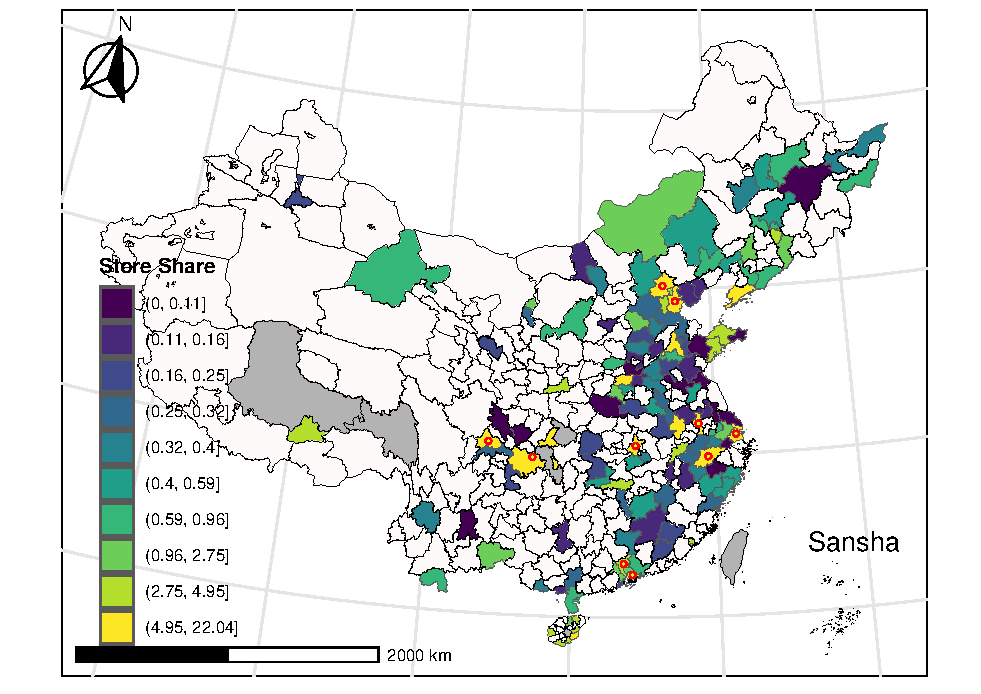
\includegraphics[width=0.7\textwidth]{../figures/distribution_of_cities_share.pdf}
  \caption{Distribution of Lianjia's Stores' Percentage across China}
  \label{fig:precise_proportion_contraction}
  Note: This plot displays the percentage of Lianjia's offline stores in each city relative to the total number of brokerages in that city, based on data from AutoNavi Map. Gray areas indicate invalid information, while white areas denote cities without any Lianjia stores. Additionally, Sansha city is featured in the bottom right corner of the graph. The base map is sourced from the AutoNavi Map.
\end{figure}

Additionally, in the China's real estate market, brokerages still operate on a bilateral agency model, where sellers need to choose the agency that can help them sell their home in the fastest time and for the highest price possible for the transaction. However, due to the asymmetric information inherent in the real estate market, sellers face challenges in effectively informing and matching with potential buyers. In a perfectly competitive market, sellers would be indifferent in their choice of real estate agents. Nonetheless, as the market trends toward increased monopolistic competition, sellers confront a dichotomous decision: engage a larger brokerage firm, which, despite higher fees, offers the potential for expedited transactions, or opt for a smaller brokerage with lower fees but potentially less efficient transaction facilitation.

While sellers might consider a co-listing strategy—listing their property with multiple brokerages—this approach is suboptimal for several reasons within China's real estate market. Despite previous literature, such as \citep{RePEc:kap:jrefec:v:67:y:2023:i:3:d:10.1007_s11146-021-09858-w}, indicating that the co-listing can be beneficial for clients under multiple-listing service. Specifically in China's real estate market, firstly, the exclusivity of contracts between sellers and agents often precludes the adoption of a co-listing strategy. Secondly, although sellers can list their properties with multiple brokerages, smaller agencies frequently lack a sufficiently broad client base, limiting their effectiveness in selling homes. Thirdly, engaging multiple brokers simultaneously can lead to reduced incentives among agents, as they perceive competition for the same property, diminishing their proactive efforts. Finally, while service cost variations between agencies are acknowledged, these costs are minor compared to the property's value and are more closely related to the risks associated with holding a financial asset. Consequently, risk-averse sellers are inclined to choose an agency that provides a guaranteed level of service. 

Given the dual nature of online promotion and offline transactions in the real estate brokerage industry, the quality of offline services is crucial for influencing client decisions. This principle underpins Lianjia's strategy of establishing numerous stores within targeted communities. By opening a wide range of stores in various neighborhoods and adopting a downstream consolidation model through platform design, the brokerage effectively attracts sellers to list their properties and buyers through its extensive platform resources. This strategy not only enhances transaction volume but also increases income derived from these transactions.

In this paper, we empirically estimate the effects of offline store clustering and online platform consolidation in China's second-hand real estate market. Utilizing micro-level transaction data, we construct our research sample by aggregating information at the neighborhood level. We employ a regression discontinuity design (RDD) to identify the optimal influential radius of offline stores on neighborhood transactions, finding that this radius corresponds to a brokerage's five-minute walk service distance, which is also documented in similar fields \citep{AZMI2012406}. Subsequently, we apply a difference-in-difference (DID) estimation method to evaluate the exogenous impact of Lianjia's market entry on local segments. This exogenous effect captures the clustering impact of offline real estate brokerage stores. Our results indicate that Lianjia's offline stores significantly enhance transaction revenues, although this effect diminishes during and after the COVID-19 period.

To evaluate the effects of platform-mediated consolidation, we consider the year Lianjia implemented its platform-mediated consolidation strategy as an exogenous shock to the market. This strategy primarily revolves around the ACN framework of Lianjia and the incorporation of various franchise stores into the network. Our empirical analysis indicates that this strategy significantly increases revenues and enhances the attraction of buyers and sellers, particularly in the number of house tours facilitated by the brokerage. However, our findings suggest that the platform-mediated consolidation does not effectively reduce the transaction period nor does it promote price concessions. This contrasts with the offline expansion strategy, which demonstrates a positive impact on promoting price concessions. While the economic impact of the online-based consolidation strategy is not as pronounced as that of the offline expansion strategy, it remains economically significant.

According to Lianjia's IPO prospectus, the company is projected to achieve approximately 76\% of cross-store transactions in 2021. This underscores the necessity of analyzing the network effects among Lianjia's offline stores and conducting a detailed examination of these effects. To assess Lianjia's network effect, we propose a measure of the local network effect by incorporating neighborhoods and offline stores, given that offline stores predominantly cluster around neighborhoods. We employ a Breadth-First Search (BFS) algorithm to construct the network formation and propose a gravity-based measure to evaluate the offline clustered network effect on neighborhoods. Additionally, we examine the impact of online-mediated consolidation on the offline stores' network effect on neighborhoods. Our findings reveal that Lianjia's offline stores exhibit a moderate network effect characterized by local clustering patterns.\footnote{\ref{fig:typical_sample_lianjia} shows a typical observation in Chengdu that two proximate Lianjia stores closely cooperate to manage property listings. In this arrangement, agents have the flexibility to bring customers for house tours.} Furthermore, the platform-mediated consolidation significantly enhances the network effect, indicating that this consolidation strategy effectively strengthens the network effect of Lianjia's offline stores. Lastly, the result also confirms that the clustering within a small segmented market allows the company to coexist with competitors, with the large company satisfying the majority of customers while other firms cater to heterogeneous customer needs. Lianjia does not exclude other brokerages from the market, but rather coexists with them, thereby enhancing the overall market competitiveness.\footnote{This finding is consistent with the study by \citep{gilbukh_goldsmith-pinkham_2019}, which indicates that inexperienced intermediaries hold a large market share, but their transaction efficiency is lower compared to experienced intermediaries.}

The structure of the paper is organized as follows. Section \ref{sec:literature_review} provides a comprehensive review of the relevant literature. Section \ref{sec:data} outlines the study's background, including a statistical summary and stylized facts. Section \ref{sec:mechanism_design} examines the impact of Lianjia's offline store expansion and platform-mediated consolidation on transaction properties.. Section \ref{sec:network_effect} details the measurement of local network effects and analyzes the influence of platform-mediated consolidation on these effects. Finally, Section \ref{sec:conclusion} discusses the findings and offers concluding remarks.

\section{Literature Review} \label{sec:literature_review}

The literature on the real estate market, particularly the role of real estate brokerages, is extensive and informative, starting with the foundational work of \citep{Rosen_hedonic} who introduced the hedonic pricing model. This model breaks down property prices by analyzing internal and external factors. However, it's worth noting that this model does not adequately account for market asymmetries and information disparities, leading to potential inaccuracies in pricing. A fundamental study by \citep{Akerlof_1970} highlights the significant impact of asymmetric information on market dynamics, using the market for used cars as an example. Here, the prevalence of low-quality goods, known as `lemons', often leads to market inefficiencies, a problem that is mirrored in the real estate sector. The challenge of asymmetric information in real markets was further emphasized by \citet{grossman_impossibility_1980}, who questioned the feasibility of the effective market assumption, particularly under conditions of information disparity. 

Subsequent studies have expanded on these foundational theories, exploring dynamics specific to real estate pricing and strategic behavior. \citet{550a6ccf-cde2-3dd1-979f-1a8db2b8ceb9} documents that apart from price competition in the market, there is a lot of market inefficiency that stems from non-price competition, which suggests that as the degree of competition in the market increases, the market becomes progressively less efficient, indicating that the entry dividend begins to fall and aggregate social welfare begins to decline. Moreover, \citet{hendel_relative_2009} analyzes two types of listings in the second-hand housing market and finds that For-Sale-By-Owner type of platforms are less effective in terms of time and probability of sale while operating better compared to listing homes for sale as a broker. In addition, \citet{bailey_economic_2018} uses data from the social media site Facebook to show that social interactions can influence people's economic decisions. Their results show that people who have friends who are geographically distant in real life and who have a hunch that house prices are about to rise are more likely to buy a house than rent one. Other relevant areas of research include \citep{SIRMANS1991207, NIEUWERBURGH_information, salz_intermediation_2022}.

The strategic behavior of real estate brokerages has been documented to leverage informational advantages. \citet{AGARWAL2019715} confirms that brokerages, as market intermediaries, possess nuanced knowledge of market conditions, enabling them to negotiate discounts effectively. Furthermore, \citet{HAN2015813} discusses the varying bargaining power of brokerages across unidirectional and bidirectional markets, influencing their operational strategies. This is corroborated by evidence suggesting that properties listed with lower commission rates not only sell less frequently but also take longer to sell \citep{10.1257/app.20160214}. Additionally, studies have documented that brokerages may adopt discriminatory strategies, steering minorities into neighborhoods with lower economic opportunities and higher exposures to crime and pollution, thereby contributing to persistent social and economic inequalities in the United States \citep{RePEc:ucp:jpolec:doi:10.1086/720140}. The advent of online platforms has significantly altered the landscape of real estate transactions. \citet{ZUMPANO2003134} notes that while the duration of property searches has not changed markedly, the scope of searches has broadened to encompass more online listings. Moreover, \citet{ZHANG2021101104} associates the rise of online platforms with a reduction in existing house prices and an increase in sales volumes, a dynamic influenced by factors such as new house prices and household demographics. However, a detailed analysis of the impact of the presence of these platforms on market performance of offline stores remains scant.

Moreover, the overall market influence of real estate intermediaries is multifaceted. Utilizing a model predicated on perfect competition, \citet{williams_agency_1998} illustrates that excessive entry of brokers into the market can surpass the optimal allocation, thereby reducing social welfare. This is corroborated by studies indicating that an increase in the number of brokers can depress house prices and shorten transaction cycles \citep{https://doi.org/10.1002/jae.2891}. Additionally, \citet{qu_identifying_2021} highlights the moderating role of broker commissions in disseminating information during transactions, facilitating more efficient home sales. Lastly, \citet{AGARWAL2024103668} utilized second-hand real estate transaction data from Beijing to demonstrate that real estate agents may significantly contribute to the formation of Yin-Yang contracts. They quantified the magnitude of the resulting tax evasion, attributing it to the learning-by-doing effect and peer influence among agents. However, their study lacked a spatial analysis component that would consider the local network effects. Other related literature includes \citep{doi:10.1080/10527001.2021.2016340, d082a2db-5cce-33f2-87c4-9cb020cc6666, doi:10.1080/10835547.1996.12090852}.

Finally, the concept of the platform as a "two-sided market" or kind of intermediates that connects the buyer side and seller side digitally, \citep{10.1162/154247603322493212, Langley_Leyshon_2017, 10.1257/aer.100.4.1642}. \citet{https://doi.org/10.1111/j.1756-2171.2006.tb00036.x} characterizes real estate brokerages as a two-sided market. In this model, brokerages must effectively communicate and mediate between sellers and buyers, facilitating transactions and ensuring efficient market operations. Despite the significant attention given to online platforms and real estate broekerage's two-sided market \citep{10.1257/jep.23.3.125}, there is a lack of systematic analysis on the impact of offline stores of online platforms on market performance or on real estate brokerage. Therefore, this paper aims to fill this gap by examining the influence of offline stores associated with online platforms on the real estate market.

Based on the study of existing literature, this paper represents the pioneering empirical investigation into the effects of offline store expansion and platform-mediated consolidation within the real estate brokerage market. Furthermore, it is the first to analyze the local network effects within the specific context of real estate transactions. Additionally, this paper systematically examines how informational advantages can enhance brokerage revenue within the framework of local network effects. By delving into these dynamics, we aim to contribute to the broader economics literature by providing a nuanced understanding of how offline and online integration influences market behavior and outcomes. Our findings offer meaningful insights into the strategic decisions of real estate brokerages, highlighting the significance of network effects and informational advantages in shaping competitive advantage and market performance. This research not only fills critical gaps in the literature but also provides a comprehensive framework for future studies to explore the intersection of offline expansion, digital consolidation, and local network effects in various economic contexts. By systematically examining these phenomena, we enhance the understanding of how technological and infrastructural developments can drive revenue generation and market consolidation in the real estate industry and beyond.

\section{Data and Descriptive Evidence \label{sec:data}}

\subsection{Data Collection and Processing} \label{subsec:data_collection}

This study focuses on the housing markets in ten major cities in China, namely Beijing, Shanghai, Chongqing, Tianjin, Shenzhen, Guangzhou, Chengdu, Hangzhou, Wuhan and Nanjing. These cities are not only pivotal to China's economic development, but also serve as exemplars of the broader trends and characteristics inherent in the China's real estate dynamics. Spanning from 2016 to 2022, the research period encapsulates a pivotal era in China's real estate sector. During the first phase of the study, from 2016 to 2019, the housing markets in these cities experienced a remarkable boom. This period was characterized by significant growth in property prices, supported by robust economic expansion and increased demand in these urban centers. However, the final phase of our study, from 2020 to 2022, paints a contrasting picture. During this period, China's overall economic growth rate has been slower significantly, which has also reflected in a slowdown in the real estate markets of these major cities. In addition, the Chinese government has implemented strict rules in Covid-19 protection and an unprecedented suite of new policies to prevent house prices from falling, so the real estate agents in these major cities are significantly affected.

The second hand housing transaction data was collected form \href{https://www.ke.com/city/}{beke.com} for ten cities ranging from 2016 to 2022.\footnote{Due to government policy, Lianjia was unable to disclose transaction prices in Beijing, Shenzhen, and Wuhan for the years 2021 and 2022, as well as in Chengdu for 2021. Consequently, we have excluded this period of data for these cities from our analysis.} Initially, we filtered out transaction records exhibiting unusually high prices, identifying them as outliers that could skew the analysis. We then removed records with missing values to maintain the integrity of our dataset. We also removed any records that were listed duplicated. We finally have a data with length 1,778,647 second-hand houses.\footnote{Due to government restrictions, four of these cities did not list the transaction price for each transaction during the study period.} After cleaning the data, we constructed two research samples: one at the individual transaction level and the other at the neighborhood level. The individual transaction sample contains detailed information on each transaction, including the transaction price, transaction date, price concessions, and the transaction period. The neighborhood-level sample aggregates transaction data at the community level, encompassing variables such as the average transaction price and the average number of house tours. Additionally, we calculated the annual number of house transactions to capture Lianjia's transaction activity within each neighborhood. We also calcualted the revenue of each neighborhood for each year by the formula: $\text{annual transaction number} \times \text{average transaction price} \times \text{brokerage fee}$ where the brokerage fee is set at 2.7\% as the majority of houses in our research sample are charged at this uniform rate. This data enables us to carry out a comprehensive analysis of the impact of offline stores on housing transactions across both individual and neighborhood dimensions.

To gather additional characteristic information, Point of Interest (POI) data was extracted from the AutoNavi map using a web-scraping Python program.\footnote{AutoNavi, a leading mapping application in China with a user base exceeding 700 million, is renowned for its detailed and accurate POI data as well as precise public transportation information. These features underscore AutoNavi's leadership in the digital mapping sector, highlighting its ability to provide unparalleled navigation accuracy and comprehensive urban mobility solutions. Our extracted AutoNavi dataset includes over one million POIs per city annually.} The extracted POIs were then classified into various categories, as detailed in Table \ref{tab:statistical_district} and Table \ref{tab:statistical_individual} and it primarily represents living facilities, entertainment venues, restaurants, hospitals, and other public amenities. This classification is crucial for understanding the urban infrastructure and amenities available in the vicinity of the analyzed properties.

Each type of POI, excluding brokerages offline stores information, was matched to our data within a 500-meter radius, a distance typically covered by walking and consistent with urban planning standards for accessible urban design.\footnote{We chose a 500-meter radius because the existing literature does not specifically document whether these types of points of interest (POIs) adhere strictly to the 5-minute walk policy. Furthermore, several studies have utilized a 500-meter radius to examine the influence of various types of POIs, including: \citep{LI2019165, doi:10.1287/mnsc.2019.3550}} This radius reflects the immediate urban environment influencing residential desirability and property values, as most of these POIs provide recreational services. Additionally, geo-informational data, including annual GDP data from \citet{zhao_forecasting_2017}, nighttime lights data from \citet{elvidge_annual_2021}, and air pollution data from \citet{doi:10.1021/acs.est.1c05309}, was integrated into our research. The centroid of the neighborhood-level data's polygon was generated, and values from the geo-informational data were extracted. By merging these data sources with our research panel, a comprehensive research sample was constructed.

\subsection{Influential Radius} \label{subsec:Influential_Radius}

The effectiveness of an offline intermediary's influence on its immediate communities is inherently constrained by geographic limitations, with its influence decreasing in proportion to the increase in spatial distance. Moreover, since the offline stores of Lianjia are directly operated by the company, strategic considerations regarding the optimal distance between stores are an integral part of their location planning to mitigate the risks associated with over-concentration of stores that could lead to competitive overlap and service homogenization. Consequently, it is imperative to determine an optimal radius threshold and subsequently assess the diversity of agencies operating within this demarcated zone.

To determine the optimal radius of influence, this research employs a RDD on the neighborhood level transaction data to examine the influential radius of offline real estate brokerages. The dependent variable in this analysis is the transaction revenue generated by Lianjia within a given community, while the independent variable is the community's proximity to the nearest Lianjia store. Given that stores are predominantly located within commercial districts, which typically encompass several streets no more than two kilometers in diameter, it is assumed that a requisite number of stores within each district is essential to sustain revenue generation in that community. In addition, Lianjia adopts a pedestrian shed strategy, also known as a 5-minute walking distance (approximately 400 meters) strategy, which means that customers should be accessible within a 5-minute walk to the nearest Lianjia store to reduce the visiting cost. Moreover, this is consistent with the govvernment's proposal policy that most of the living facilities should be within five-minute pedestrian scale distance \citep{GB50180-2018}. Besides, some other paper also demonstrated that in other fields, the distance above 5-minute walk distance can create significant drop in most of the properties \citep{liu2023chrono-urbanism}.

Building on this premise, the study further investigates the existence of an optimal influence radius within shopping districts, defined as the distance radius within which the presence of a Lianjia optimally increases transaction revenues. At the same time, the study also examines the hypothesis that beyond this optimal radius, the impact on transaction revenues diminishes as a result of the strategic store layout decisions implemented by Lianjia.

\begin{figure}[ht]
    \centering
    \subfloat[RDD plot with first order polynomial]{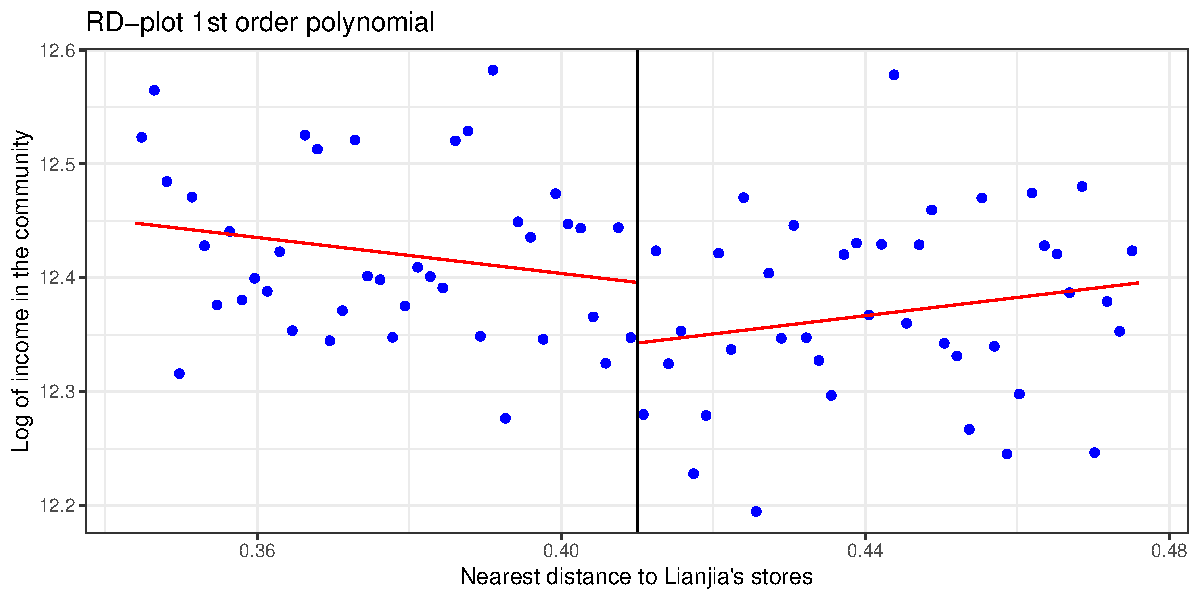
\includegraphics[width=0.5\textwidth]{../figures/RD_Plot_1st_Order.pdf}\label{fig:RD_Plot_1st_Order}}
    \hfill % Adds horizontal space between figures
    \subfloat[RDD plot with second order polynomial]{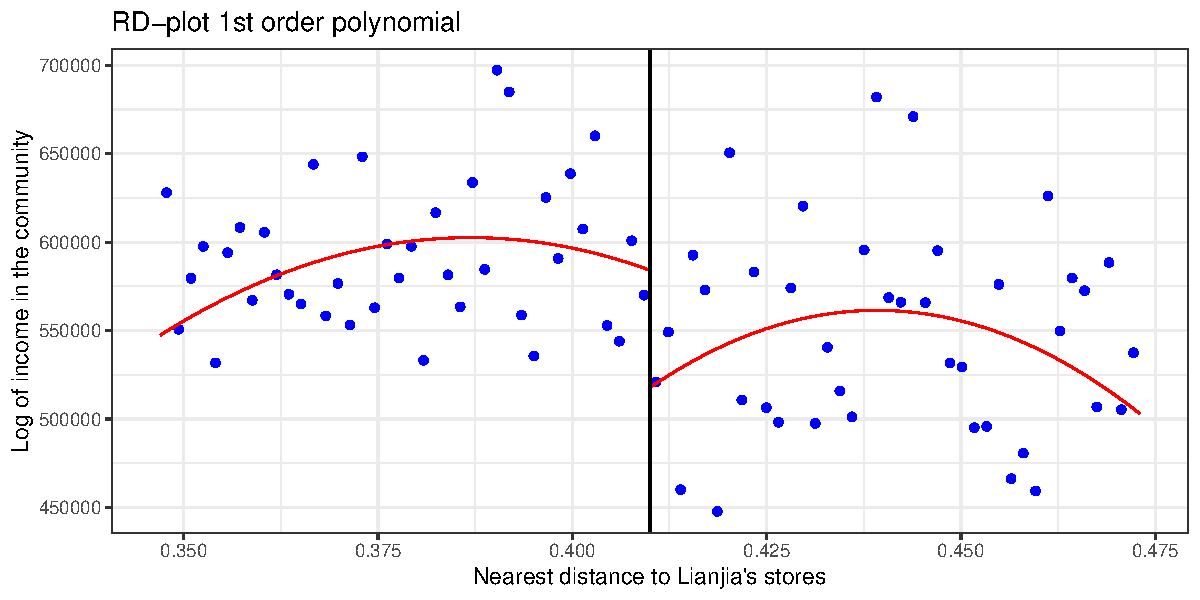
\includegraphics[width=0.5\textwidth]{../figures/RD_Plot_2nd_Order.pdf}\label{fig:RD_Plot_2nd_Order}}
    \hfill % Adds horizontal space between figures
    \subfloat[RDD plot with third order polynomial]{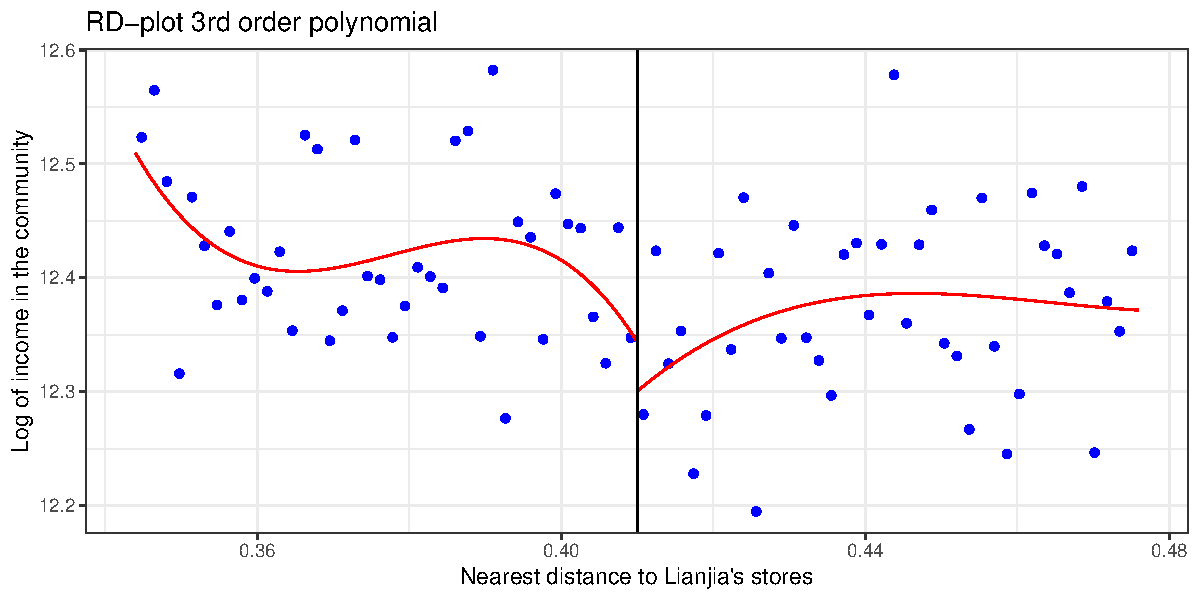
\includegraphics[width=0.5\textwidth]{../figures/RD_Plot_3rd_Order.pdf}\label{fig:RD_Plot_3rd_Order}}
    \caption{RDD with Different Polynomial Orders}
    \label{fig:RD_design}

    Note that the running variable is divided into 40 bins, considering only the samples within the specified bandwidth. The polynomial order for the RDD analysis ranges from 1 to 3. Each plot illustrates the relationship between the community transaction revenue and the nearest distance to Lianjia's stores, with the discontinuity point at the cutoff.
\end{figure}

% latex table generated in R 4.2.0 by xtable 1.8-4 package
% Mon Jul  8 21:12:27 2024
\begin{table}[ht]
\centering
\begin{tabular}{lllllllr}
  \hline
Method & Kernel & Estimate & SE & Z & PValue & Bandwidth & EffectiveObs \\ 
  \hline
mserd & uniform & -48903 & 21529 & -2.27 & 0.0231 & 0.0504 & 24269 \\ 
  mserd & triangular & -61304 & 20887 & -2.94 & 0.00333 & 0.063 & 30532 \\ 
  cerrd & uniform & -56899 & 28636 & -1.99 & 0.0469 & 0.0273 & 13166 \\ 
  cerrd & triangular & -59561 & 27943 & -2.13 & 0.033 & 0.0341 & 16392 \\ 
   \hline
\end{tabular}
\caption{RD Estimates with Different Bandwidth Selection Methods and Kernels} 
\label{tab:rd_bandwidth_kernel_results}
\end{table}



From Figure \ref{fig:RD_design} we can see that there is indeed discontinuity in 410 meters of communities to the nearest Lianjia's store, which is pretty close to the Lianjia's 5-minute walk distance policy (approximately 410 meters). The observed decline in the Lianjia's influence is marked and suggests a pronounced reduction in its impact on the system overall within our study sample. This phenomenon can be attributed to the implementation of the Lianjia's proximity to customers policy, which is evidenced at the data level. Table \ref{tab:rd_bandwidth_kernel_results} considers different kernel and bandwidth choices, and the results are consistent with the 410 meters radius. The results are robust to different bandwidth and kernel choices, which suggests that the 410 meters is the optimal radius for Lianjia's offline stores.\footnote{It is important to note that we should avoid using bandwidths that correspond to distances too small relative to the proximity between Lianjia stores and neighborhoods. This is because our evaluation of neighborhood proximity is based on the centroid of each neighborhood. The distance from a store to the centroid does not necessarily imply that the store is not close to the neighborhood itself. Therefore, when distances are very close to the neighborhood centroid, it is reasonable to consider the store as approximately close to the neighborhood as well.} To check the robustness of the results, we conducted a series of robustness checks. The results are shown in Appendix \ref{sec:additional_rdd}.

To check the robustness of our results, we first consider transforming the dependent variable by taking its natural logarithm. This transformation is intended to account for the possibility that the functional form of the dependent variable may affect the estimation of the treatment effect. By using the natural logarithm, we aim to normalize the distribution and potentially stabilize the variance, which could lead to more reliable estimates. We repeat the procedures described in the main analysis using this transformed dependent variable. The corresponding results are presented in Appendix Figure \ref{fig:RD_design_Robust} and Appendix Table \ref{tab:rd_bandwidth_kernel_results_robust}. Our findings indicate that the results remain consistent with those obtained using the original dependent variable. This consistency suggests that the treatment effect is robust to changes in the functional form of the dependent variable. Furthermore, the analysis reaffirms that a 410-meter radius remains the optimal bandwidth for assessing the impact of Lianjia's offline stores. This robustness check enhances the credibility of our main findings and supports the validity of the 410-meter radius as a critical threshold for evaluating proximity effects.

One another common concern in RDD is the potential for manipulation around the cutoff, which could invalidate the results. To address this, a falsification testing based on ``Donut Hole'' specifications can be implemented, where observations close to the cutoff are excluded to ensure that the results are not driven by manipulation or other local irregularities. 
In this study, we conduct a robustness check using the Donut Hole method on a RDD with a cutoff at 410 meters. Specifically, we sequentially exclude observations within certain distances from the cutoff and re-estimate the treatment effect. The distances considered for exclusion are 5, 7.5, 10, 12.5, 15, 17.5, 20 meters, and they are correspondingly dropping 7.85\%, 11.73\%, 15.59\%, 19.48\%, 23.66\%, 27.88\% and 31.71\% of our effective estimation data, respectively. Appendix Table \ref{tab:rd_robust_results} indicate that up to the exclusion of 20\% of the estimated data, the treatment effect estimates remain consistent and robust, thereby demonstrating the robustness of the estimated treatment effects to the exclusion of data points near the cutoff. Moreover, we find that adding control variables may help us to better estimate the treatment effect and make our model more robust.

Furthermore, we carry out the density test by \citep{MCCRARY2008698}. The McCrary test checks whether there is a discontinuity in the density of the running variable at the cutoff point. A significant discontinuity would suggest that individuals or entities have manipulated the running variable to either side of the cutoff, thereby violating the assumption of no manipulation. The results are shown in Appendix Table \ref{tab:mccrary_results} shows that the p-value is greater than 0.1, which suggests the result is not due to manipulation of polygons.

To ensure that the observed treatment effect at the true cutoff is not a result of underlying trends or other spurious factors. We first check to identify any potential confounding variables that might be driving the results instead of the treatment effect. To achieve this, we conducted a placebo test by substituting the dependent variable with other control variables and the results are shown in Appendix Table \ref{tab:placebo_test_results}. The results suggest that the discontinuity does not exist in the placebo test, which substantiates that the observed discontinuity is not due to any general discontinuity in the data at the cutoff but is specifically attributable to the treatment effect.

We also conducted a series of placebo tests by systematically adjusting the cutoff points to 325 meters, 350 meters, 400 meters, 420 meters, 450 meters, 500 meters, 650 meters, and 700 meters, in addition to the original cutoff at 410 meters. These adjustments aimed to assess the robustness and specificity of the intervention's impact. The results, presented in Appendix Table \ref{tab:movement_cutoff}, reveal that the estimated effects are statistically significant at the 400-meter, 420-meter, and 450-meter cutoffs, with the estimated coefficients demonstrating consistency across these points. In contrast, when the cutoff is set at shorter distances (325 meters and 350 meters) or longer distances (500 meters, 650 meters, and 700 meters), the effects diminish and lose statistical significance. This pattern suggests that the impact of the policy or intervention is localized and concentrated around the 410-meter threshold, providing strong evidence for the validity of this specific cutoff point.

Furthermore, the consistency of significant results at cutoffs close to 410 meters (specifically at 400 meters and 420 meters) reinforces the robustness of our findings. It suggests that small variations around the original cutoff do not substantially alter the observed effects, underscoring the reliability of the 410 meter cutoff as a meaningful cutoff. The lack of significant effects at more distant cutoffs suggests that the influence of the intervention does not extend beyond a certain distance, highlighting its localized nature.

\subsection{Statistical Summary} \label{subsec:Statistical_Summary}

After constructing our optimal radius, we recalcualte the number of Lianjia and other brokerages' stores within this radius. To check the robustness of the data, we divide our data to those with Lianjia and those without Lianjia and to check whether Lianjia's offline stores have influential effect on the transaction effect in the neighborhoods. We can see that for transaction numbers, income, number of house tours and price concession are all significantly different in those neighborhoods with or without Lianjia. In addition, we find that the other brokerages also have the same tendency that they typically open stores with the same strategy as Lianjia, which suggests that Lianjia does not have the market power to exclude competent companies from entering the market, and it also suggests that the market is not monopolized by Lianjia. We plot the relationship between the number of other brokerages's stores and the number of Lianjia's stores and the figure is shown in Figure \ref{fig:same_distribution}. The figure shows that the the number of other brokerages' stores is positively correlated and the general trend tends to be linear, which further suggests that the market is not monopolized by Lianjia.

From Table \ref{tab:statistical_district} we can see that in our metro areas, the neighborhoods with Lianjia within the influential radius tends to have higher number of sales, and the final transaction price is also \textyen 910,000 (approximately 35\%) higher than those neighborhoods without Lianjia. Moreover, the number of other stores within the influential distance is also signnificantly more than 7.3, which also aligns with our previous intuition that the market is not monopolized by Lianjia. This significance difference suggests that if we treat our sample as a cross sectional data and estimate the result with static model without considering the individual fixed effect, we may get a biased result. Besides, our model may suffer from endogeneity issue, since the number of Lianjia's stores may be endogenous to the transaction price and the number of stores. 

\begin{table}[htb!]
    \centering
    \begin{tiny}
    \caption{Statistical Summary for the Neighborhoods-Data with Lianjia and without Lianjia}
    \begin{tabular}{llllll}
\toprule
Name & Mean without lianjia & SD without lianjia & Mean with lianjia & SD with lianjia & Difference \\
\midrule
\multicolumn{6}{l}{\textbf{Panel 1: }Transaction property} \\
income & 44.44 & 73.85 & 77.68 & 117.3 & -33.24 (-76.638***) \\
lead\_times & 13.59 & 14.56 & 17.09 & 17.50 & -3.501 (-49.823***) \\
price\_concession & -0.0367 & 0.0318 & -0.0351 & 0.0294 & -0.00200 (-12.088***) \\
\multicolumn{6}{l}{\textbf{Panel 2: }brokerage property} \\
density & 0 & 0 & 0.206 & 0.166 & -0.206 (-384.429***) \\
broker\_410 & 5.362 & 6.871 & 12.66 & 8.410 & -7.300 (-217.614***) \\
watching\_people & 17.61 & 29.11 & 20.29 & 29.40 & -2.682 (-21.214***) \\
end\_price & 260.5 & 254.9 & 351.9 & 292.1 & -91.48 (-76.662***) \\
non\_online\_effect & 0.195 & 0.396 & 0.233 & 0.423 & -0.0380 (-21.384***) \\
watched\_times & 1121 & 1827 & 1233 & 1969 & -112.4 (-13.636***) \\
nego\_times & 4.769 & 7.686 & 5.683 & 10.78 & -0.914 (-22.178***) \\
nego\_period & 150.5 & 187.5 & 166.6 & 239.1 & -16.06 (-17.075***) \\
\multicolumn{6}{l}{\textbf{Panel 3: }hedonic information property} \\
jiadian & 1.489 & 3.566 & 1.942 & 4.365 & -0.453 (-26.004***) \\
kind & 8.665 & 6.229 & 11.76 & 6.081 & -3.097 (-116.630***) \\
hotel & 3.211 & 5.287 & 5.428 & 6.315 & -2.217 (-87.264***) \\
shop\_mall & 4.554 & 7.539 & 6.698 & 8.489 & -2.144 (-61.405***) \\
museum & 0.617 & 1.533 & 1.023 & 1.869 & -0.406 (-54.395***) \\
old & 0.894 & 1.628 & 1.339 & 1.950 & -0.446 (-56.870***) \\
ktv & 5.179 & 7.853 & 7.305 & 7.759 & -2.126 (-63.096***) \\
mid & 2.059 & 2.329 & 3.368 & 2.853 & -1.309 (-115.077***) \\
prim & 2.812 & 2.846 & 4.343 & 3.205 & -1.531 (-116.172***) \\
west\_food & 3.880 & 7.709 & 7.317 & 10.02 & -3.437 (-87.756***) \\
super & 3.155 & 3.374 & 4.499 & 3.686 & -1.344 (-87.586***) \\
sub & 0.683 & 0.945 & 1.111 & 1.099 & -0.429 (-96.038***) \\
park & 3.422 & 4.575 & 4.569 & 3.944 & -1.147 (-62.708***) \\
\multicolumn{6}{l}{\textbf{Panel 4: }house property} \\
area & 90.82 & 48.57 & 84.97 & 39.15 & 5.845 (31.050***) \\
bedroom & 2.338 & 0.816 & 2.202 & 0.730 & 0.136 (40.958***) \\
toilet & 1.306 & 0.579 & 1.246 & 0.455 & 0.0600 (26.915***) \\
house\_age & 18.08 & 11.68 & 20.73 & 11.77 & -2.651 (-52.316***) \\
floor\_level & 1.854 & 0.975 & 1.933 & 0.931 & -0.0790 (-19.324***) \\
green\_ratio & 0.309 & 0.237 & 0.300 & 0.107 & 0.00900 (12.288***) \\
total\_building & 26.88 & 56.66 & 20.51 & 50.54 & 6.371 (27.653***) \\
total\_floor\_number & 12.75 & 8.454 & 12.97 & 8.485 & -0.221 (-6.035***) \\
living\_room & 1.445 & 0.504 & 1.341 & 0.492 & 0.104 (48.345***) \\
elevator\_ratio & 0.453 & 0.413 & 0.408 & 0.279 & 0.0450 (30.475***) \\
kitchen & 0.983 & 0.150 & 0.983 & 0.125 & 0 (-0.459) \\
floor\_ratio & 4.942 & 329.1 & 2.702 & 9.385 & 2.240 (2.367**) \\
\multicolumn{6}{l}{\textbf{Panel 5: }regional property} \\
total\_resident & 995.8 & 1079 & 901.8 & 956.5 & 93.97 (21.484***) \\
pm25 & 44.08 & 13.29 & 45.74 & 13.89 & -1.664 (-28.266***) \\
pop & 15506 & 16336 & 24634 & 18866 & -9100 (-118.769***) \\
light & 32.62 & 13.59 & 38.41 & 11.92 & -5.782 (-105.485***) \\
\bottomrule
\end{tabular}

    \label{tab:statistical_district}

    Note that the code book of the variables can be seen in the Appendix \ref{tab:codebook} and with or without Lianjia represent whether there are Lianjia's offline stores within the influential radius.
    \end{tiny}
\end{table}

\begin{table}[htb!]
  \centering
  \begin{tiny}
  \caption{Statistical Summary for the Individual-Data with Lianjia and without Lianjia}
  \begin{tabular}{llllll}
\toprule
Name & Mean without lianjia & SD without lianjia & Mean with lianjia & SD with lianjia & Difference \\
\midrule
\multicolumn{6}{l}{\textbf{Panel 1: }Transaction property} \\
income & 0.493 & 0.656 & 0.797 & 0.974 & -0.304 (-226.763***) \\
lead\_times & 16.83 & 26.13 & 20.47 & 31.23 & -3.648 (-80.341***) \\
price\_concession & -2.791 & 2.984 & -2.703 & 2.776 & -0.0890 (-19.908***) \\
\multicolumn{6}{l}{\textbf{Panel 2: }brokerage property} \\
density & 0 & 0 & 0.235 & 0.182 & -0.235 (-1.1e+03***) \\
broker\_410 & 4.620 & 6.135 & 11.39 & 7.999 & -6.765 (-596.183***) \\
watching\_people & 18.49 & 59.53 & 22.13 & 49.02 & -3.647 (-44.332***) \\
end\_price & 229.8 & 197.1 & 305.3 & 237.0 & -75.50 (-219.538***) \\
non\_online\_effect & 0.232 & 0.422 & 0.238 & 0.426 & -0.00600 (-9.241***) \\
watched\_times & 1128 & 2226 & 1235 & 2387 & -106.8 (-29.718***) \\
nego\_times & 6.275 & 15.16 & 6.636 & 17.65 & -0.361 (-13.948***) \\
nego\_period & 139.0 & 197.5 & 141.8 & 225.4 & -2.840 (-8.544***) \\
\multicolumn{6}{l}{\textbf{Panel 3: }hedonic information property} \\
jiadian & 0.299 & 1.492 & 0.379 & 1.683 & -0.0800 (-32.152***) \\
kind & 2.253 & 2.136 & 3.347 & 2.421 & -1.094 (-305.752***) \\
hotel & 0.586 & 1.413 & 1.022 & 1.762 & -0.436 (-172.389***) \\
shop\_mall & 0.896 & 2.355 & 1.463 & 3.000 & -0.567 (-132.449***) \\
museum & 0.103 & 0.492 & 0.146 & 0.526 & -0.0430 (-53.977***) \\
old & 0.194 & 0.582 & 0.273 & 0.690 & -0.0790 (-78.187***) \\
ktv & 1.021 & 2.439 & 1.611 & 2.726 & -0.590 (-145.734***) \\
mid & 0.468 & 0.851 & 0.753 & 1.079 & -0.285 (-184.969***) \\
prim & 0.666 & 0.996 & 1.034 & 1.146 & -0.368 (-218.091***) \\
west\_food & 0.716 & 1.942 & 1.423 & 2.640 & -0.707 (-190.757***) \\
super & 2.515 & 2.959 & 3.748 & 3.356 & -1.233 (-248.593***) \\
sub & 0.143 & 0.365 & 0.247 & 0.461 & -0.104 (-158.165***) \\
park & 0.671 & 1.319 & 0.916 & 1.292 & -0.245 (-121.784***) \\
\multicolumn{6}{l}{\textbf{Panel 4: }house property} \\
area & 86.14 & 40.03 & 81.62 & 36.37 & 4.518 (77.381***) \\
bedroom & 2.285 & 0.873 & 2.145 & 0.854 & 0.140 (105.281***) \\
toilet & 1.261 & 0.554 & 1.222 & 0.481 & 0.0400 (50.222***) \\
house\_age & 15.47 & 10.88 & 18.36 & 11.45 & -2.888 (-166.420***) \\
floor\_level & 1.851 & 0.977 & 1.890 & 0.959 & -0.0390 (-25.910***) \\
green\_ratio & 0.325 & 0.168 & 0.319 & 0.0942 & 0.00600 (31.022***) \\
total\_building & 34.11 & 64.21 & 30.05 & 67.64 & 4.061 (39.620***) \\
total\_floor\_number & 15.81 & 9.744 & 15.47 & 9.637 & 0.348 (23.296***) \\
living\_room & 1.436 & 0.574 & 1.319 & 0.575 & 0.117 (131.401***) \\
elevator\_ratio & 0.430 & 0.376 & 0.390 & 0.250 & 0.0400 (84.381***) \\
kitchen & 0.988 & 0.144 & 0.988 & 0.136 & 0 (0.385) \\
floor\_ratio & 2.923 & 124.3 & 2.738 & 6.971 & 0.184 (1.555) \\
\multicolumn{6}{l}{\textbf{Panel 5: }regional property} \\
total\_resident & 1899 & 1750 & 1903 & 1666 & -4.785 (-1.824*) \\
pm25 & 45.49 & 13.47 & 48.01 & 14.35 & -2.519 (-116.310***) \\
pop & 12369 & 14407 & 19596 & 17151 & -7200 (-289.518***) \\
light & 31.41 & 12.98 & 36.56 & 11.92 & -5.155 (-270.639***) \\
\bottomrule
\end{tabular}

  \label{tab:statistical_individual}

  Note that the code book of the variables can be seen in the Appendix \ref{tab:codebook} and with or without Lianjia represent whether there are Lianjia's offline stores within the influential radius.
  \end{tiny}  
\end{table}

\begin{figure}
    \centering
    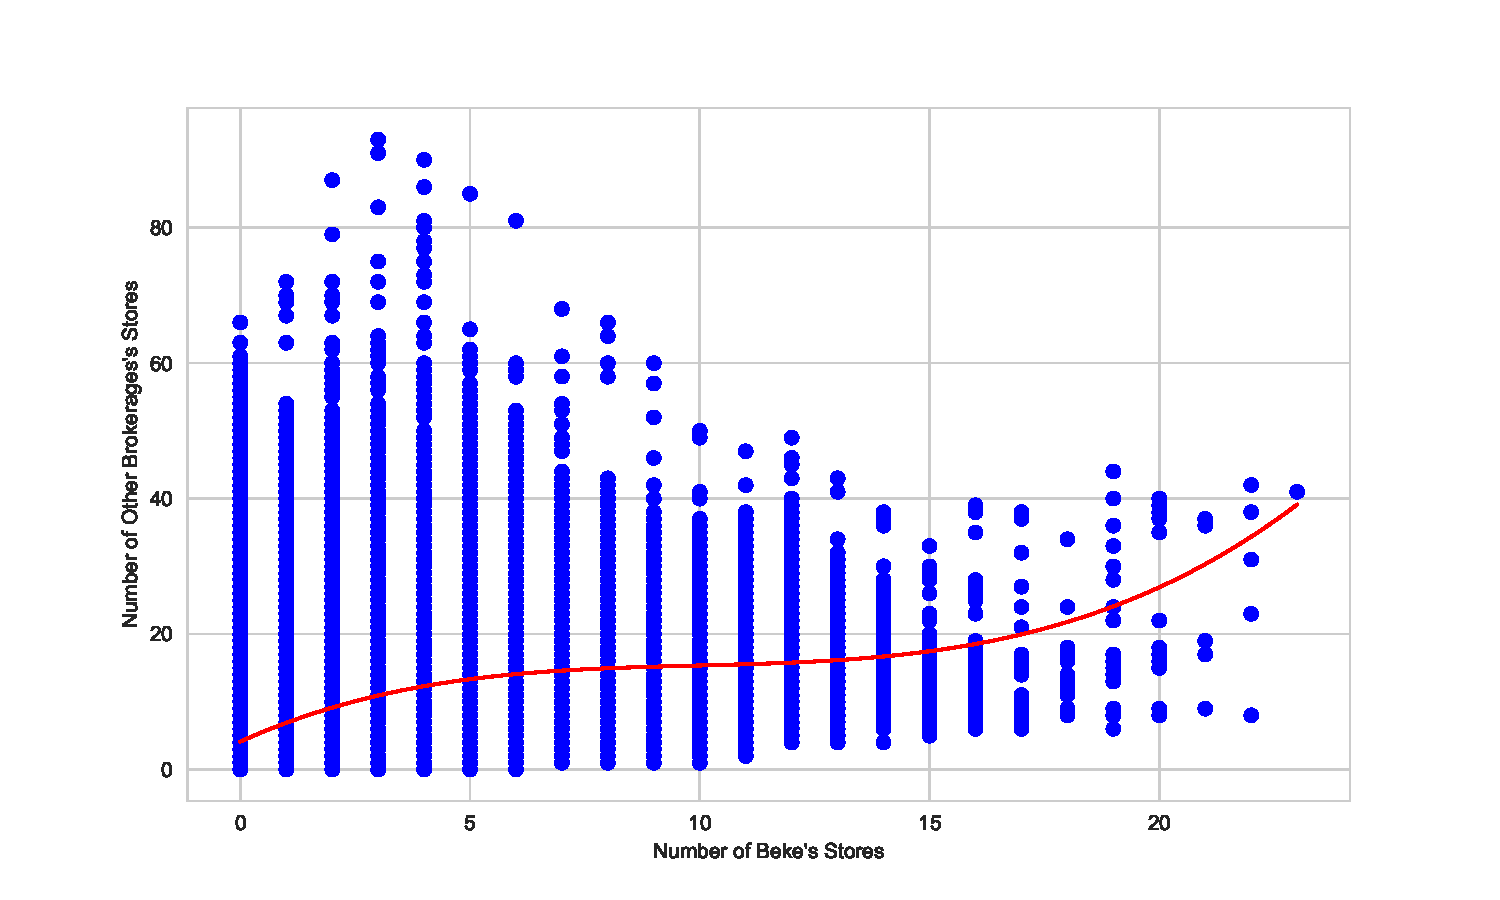
\includegraphics[width=0.7\textwidth]{../figures/scatter_plot_with_two_brokerages.pdf}
    \caption{Tendency between Two Types of Brokerages}
    \label{fig:same_distribution}
    Note: the x-axis is the number of Lianjia's stores and the y-axis is the number of other brokerages' stores. The fit is a cubic polynomial fit.
\end{figure}


\subsection{Stylized Fact} \label{subsec:stylized_fact}

In our analysis, we focus on several dependent variables: \emph{the natural logarithm of Lianjia's transaction number}, \emph{the natural logarithm of home tours}, \emph{the natural logarithm of transaction period} and \emph{the price concession}. To take the natural logarithm without lossing information, we decided to add one to the number of house tours because some transactions are purely online-based. Additionally, we decided to winsorize the sample for the natural logarithms of Lianjia's transaction number, home tours, and transaction period at the 1st and 99th percentiles to mitigate the influence of extreme values. The price concession is defined as $|\frac{\text{transaction price} - \text{listing price}}{\text{listing price}}| \times 100\%$. To quantify Lianjia's impact, we begin by establishing a key stylized fact, which we develop a Density-Based Index (DBI) index to capture the Lianjia's offline stores' influential ratio. The index is to measure the effects of Lianjia's operations and its continuous expansion. The definition of this index is informed by the results of an influential radius test, which helps us capture the spatial extent of Lianjia's influence on local real estate markets. This approach allows for a more nuanced understanding of how Lianjia's presence affects key market variables. The DBI is calculated as follows:

\begin{equation*}
  density_{it} = \frac{lianjia_{it}}{total_{it}},
\end{equation*}

where $lianjia_{it}$ represents the number of Lianjia's stores within a 410-meter radius and $total_{it}$ denotes the total number of real estate brokerages' stores within the same radius. The choice of this index is grounded in an effort to address potential reverse causality issues. Specifically, Lianjia and other brokerages often strategically place their stores in highly desirable locations, which typically also results high transaction volumes. This could potentially will caused our estimation biased if we were to simply count the number of Lianjia's stores. To deal for this issue, we employ a comparative metric: the ratio of Lianjia brokerages to the total number of real estate brokerages within the radius. This ratio helps mitigate the bias that may arise from the strategic location choices of Lianjia, offering a clearer measure of its market influence relative to competitors. This approach aligns with the principles of spatial competition theory, as articulated by \citep{hotelling_stability_1929, daspremont_hotellings_1979} in competition model. Such a comparative metric not only provides a more accurate reflection of Lianjia's market penetration but also adheres to economic modeling standards by accounting for competitive dynamics in the sector.

To capture the individual fixed effect and other time-invariant unobservable influential factors, a multi-way fixed effect model is proposed. The model is specified as follows: 

\begin{equation}
  Y_{it} = \beta_0 + \beta_1 density_{it} + \bf{\alpha} \bf{X}_{it} + \eta_{t} \times \text{bs\_code}_i + \mu_i + \epsilon_{it}, \label{eq:multi-way-fe}
\end{equation}

where $Y_{it}$ is the three main dependent variables, including $\log(\text{number})$, price concession, and $\log(\text{lead times})$, $density_{it}$ is the DBI, $\bf{X}_{it}$ are a set of control variables, including brokerage\_control Lag(hedonic\_control), transaction\_control and region\_control, while $\eta_{t} \times \text{bs\_code}_i$ is the time dummy variable interacting with the fixed effect of the business area, $\mu_i$ is the neighborhood fixed effect and $\epsilon_{it}$ is the random error term. The standard errors are clustered at the each business area level.\footnote{The business area is defined as a zone with combination of multiple neighborhoods, which Lianjia designates as the primary divisions of the entire region. The Lianjia's definition of a zone is different and typically smaller than a zone defined by the government.} The results are shown in Table \ref{tab:stylized_fact}.

\begin{table}[htb!]
    \centering
    \begin{scriptsize}
    {
\def\sym#1{\ifmmode^{#1}\else\(^{#1}\)\fi}
\begin{tabular}{l*{3}{c}}
\toprule
            &\multicolumn{1}{c}{(1)}&\multicolumn{1}{c}{(2)}&\multicolumn{1}{c}{(3)}\\
            &\multicolumn{1}{c}{log(income)}&\multicolumn{1}{c}{price concession}&\multicolumn{1}{c}{log(lead times)}\\
\midrule
density     &      0.0718\sym{***}&   -0.000542         &      0.0397\sym{**} \\
            &    (0.0203)         &  (0.000775)         &    (0.0156)         \\
\addlinespace
Other Brokerage Num  &     0.00100         &   0.0000171         &   -0.000348         \\
            &   (0.00116)         & (0.0000425)         &  (0.000781)         \\
\addlinespace
log(watch people)&      0.0662\sym{***}&     0.00189\sym{***}&       0.333\sym{***}\\
            &   (0.00378)         &  (0.000154)         &   (0.00432)         \\
\addlinespace
ln(Price)&       0.920\sym{***}&      0.0707\sym{***}&       0.240\sym{***}\\
            &    (0.0298)         &   (0.00226)         &    (0.0232)         \\
\addlinespace
log(watch time)&      0.0309\sym{***}&   -0.000237\sym{**} &      0.0318\sym{***}\\
            &   (0.00244)         & (0.0000953)         &   (0.00206)         \\
\addlinespace
log(nego changes)&      0.0240\sym{***}&     0.00202\sym{***}&       0.135\sym{***}\\
            &   (0.00635)         &  (0.000247)         &   (0.00703)         \\
\addlinespace
log(negotiation period)&      0.0598\sym{***}&    -0.00189\sym{***}&       0.131\sym{***}\\
            &   (0.00350)         &  (0.000169)         &   (0.00395)         \\
\midrule
\(N\)       &      134648         &      132301         &      134648         \\
R-squared   &       0.886         &       0.610         &       0.918         \\
\bottomrule
\multicolumn{4}{l}{\footnotesize Standard errors in parentheses}\\
\multicolumn{4}{l}{\footnotesize \sym{*} \(p<0.1\), \sym{**} \(p<0.05\), \sym{***} \(p<0.01\)}\\
\end{tabular}
}

    \caption{The DBI Influence to the Lianjia's Transaction}

    Note: we omit all the control variables in the regression model, and detailed descriptions can be seen from Table \ref{tab:statistical_district} and Table \ref{tab:statistical_individual}. In column 1 and 2, we estimated the model using the neighborhood-level data and in column 3 and 4, we estiamted the model using the individual-level data, respectively. Standard Errors are clustered at the business area level.
    \label{tab:stylized_fact}
    \end{scriptsize}
\end{table}

The results show that the share of Linajia's offline stores in total brokerage plays a significant role in the real estate market, especially in terms of number and lead time, but not in terms of price concession and transaction period. Specifically, a 1\% increase in a Lianjia's DBI within an area correlates with a 7\% increase in number, as indicated in column 1. Furthermore, this increased DBI also leads to a 4.2\% increase in the number of home tours in the column 2, underscoring the Lianjia's increased visibility and potential for customer engagement. In contrast, the analysis shows no significant effect of DBI on price concessions and transaction time. This finding suggests that while a larger share of offline stores within the segmented market increases the number of sales and the number of house tours, it may not be beneficial for mathcing the buyers and sellers, as demonstrated by the insignificance of the coefficients of log(transaction period) and price concessions. The broader implications point to the strategic advantage of density or market share in driving business performance metrics, except for customers' choices, which appear to be unaffected by changes in market share.

Within the temporal scope of our investigation, the dataset encapsulates two distinct epochs: a phase characterized by surging housing prices and the subsequent period marked by the COVID-19 pandemic. These intervals were further complicated by regulatory measures enacted by the Chinese government, significantly altering the operational dynamics and influence of brokerages within the housing market. Acknowledging these temporal shifts necessitates a nuanced analysis of the brokerage effect across different stages of the study period to ensure the robustness of our findings. To address this, we adopt a dynamic analytical approach, dissecting the period into annual segments. This granularity is achieved by constructing seven unique variables, each representing the interaction between brokerage density and the respective $density_{it} * year_{it}$. Our methodology employs a multi-way fixed effects model, as detailed in Equation \eqref{eq:dynamic}, which facilitates a comprehensive examination of temporal variations in the brokerage's market impact.

In the construction of our regression model, we deliberately omit the first period to avoid multicollinearity problem, treating it as a baseline for comparison. This strategic choice allows us to refine our proxy variable—the product of Lianjia's Dealership Balance Index (DBI) and annual dummies—as a better measure of Lianjia's local market power. Besides, to control potential self correlation problem, we also included lagged one period dependent variables in the model. Other settings are the same with the previous model \eqref{eq:multi-way-fe} and the model is described as \eqref{eq:dynamic} and the results are reported in Table \ref{tab:Dynamic}: 

\begin{equation}
  Y_{it} = \beta_0 + \rho Y_{it-1} + \sum_{i=2}^7 density_{it} * year_{it} + \bf{\alpha} \bf{X}_{it} + \eta_{t} \times \text{bs\_code}_i + \mu_i + \epsilon_{it}. \label{eq:dynamic}
\end{equation}

\begin{table}[H]
  \begin{center}
    \begin{scriptsize}
    \caption{Dynamic Regression Results}
    \label{tab:Dynamic}
    {
\def\sym#1{\ifmmode^{#1}\else\(^{#1}\)\fi}
\begin{tabular}{l*{4}{c}}
\toprule
            &\multicolumn{1}{c}{(1)}&\multicolumn{1}{c}{(2)}&\multicolumn{1}{c}{(3)}&\multicolumn{1}{c}{(4)}\\
            &\multicolumn{1}{c}{log(income)}&\multicolumn{1}{c}{log(lead times)}&\multicolumn{1}{c}{log(negotiation period)}&\multicolumn{1}{c}{price concession}\\
\midrule
year2 $\times$ density&       0.209\sym{***}&      0.0404         &      0.0639\sym{**} &   -0.000194         \\
            &    (0.0345)         &    (0.0248)         &    (0.0282)         &  (0.000592)         \\
\addlinespace
year3 $\times$ density&       0.160\sym{***}&      0.0894\sym{***}&     0.00336         &    0.000978\sym{*}  \\
            &    (0.0302)         &    (0.0226)         &    (0.0209)         &  (0.000551)         \\
\addlinespace
year4 $\times$ density&      0.0623\sym{**} &      0.0463\sym{**} &     -0.0168         &    0.000528         \\
            &    (0.0298)         &    (0.0221)         &    (0.0249)         &  (0.000501)         \\
\addlinespace
year5 $\times$ density&      0.0868\sym{***}&      0.0485\sym{**} &     -0.0581\sym{**} &    0.000331         \\
            &    (0.0307)         &    (0.0214)         &    (0.0278)         &  (0.000459)         \\
\addlinespace
year6 $\times$ density&      -0.182\sym{***}&    -0.00849         &     -0.0363         &    -0.00247\sym{***}\\
            &    (0.0540)         &    (0.0357)         &    (0.0359)         &  (0.000868)         \\
\addlinespace
year7 $\times$ density&      -0.133\sym{**} &      0.0395         &     -0.0346         &    -0.00404\sym{***}\\
            &    (0.0573)         &    (0.0493)         &    (0.0413)         &   (0.00108)         \\
\addlinespace
other brokerage num  &     0.00203\sym{*}  &    0.000597         &   -0.000995         &  0.00000271         \\
            &   (0.00107)         &  (0.000733)         &  (0.000828)         & (0.0000138)         \\
\addlinespace
ln(Price)&       0.931\sym{***}&       0.240\sym{***}&      -0.220\sym{***}&      0.0130\sym{***}\\
            &    (0.0300)         &    (0.0232)         &    (0.0210)         &  (0.000550)         \\
\addlinespace
log(watch people)&      0.0680\sym{***}&       0.328\sym{***}&       0.358\sym{***}&    0.000582\sym{***}\\
            &   (0.00377)         &   (0.00427)         &   (0.00266)         & (0.0000376)         \\
\addlinespace
log(watch time)&      0.0301\sym{***}&      0.0327\sym{***}&      0.0386\sym{***}&   -0.000587\sym{***}\\
            &   (0.00242)         &   (0.00202)         &   (0.00188)         & (0.0000296)         \\
\addlinespace
log(nego changes)&      0.0230\sym{***}&       0.133\sym{***}&       0.652\sym{***}&     0.00188\sym{***}\\
            &   (0.00635)         &   (0.00691)         &   (0.00577)         & (0.0000577)         \\
\addlinespace
log(negotiation period)&      0.0579\sym{***}&       0.126\sym{***}&                     &                     \\
            &   (0.00348)         &   (0.00388)         &                     &                     \\
\midrule
\(N\)       &      134648         &      134648         &     1771638         &     1736077         \\
R-squared   &       0.887         &       0.919         &       0.520         &       0.233         \\
\bottomrule
\multicolumn{5}{l}{\footnotesize Standard errors in parentheses}\\
\multicolumn{5}{l}{\footnotesize \sym{*} \(p<0.1\), \sym{**} \(p<0.05\), \sym{***} \(p<0.01\)}\\
\end{tabular}
}


    Note: we omit all the control variables in the regression model, and detailed descriptions can be seen from Table \ref{tab:statistical_district} and Table \ref{tab:statistical_individual}. Standard Errors are clustered at the business area level.
    \end{scriptsize}
  \end{center}
\end{table}

The result highlights the dynamic impact of offline store's share on maret performance, especially in response to external factors such as the digital transformation and the COVID-19 pandemic. Firstly, Lianjia's impact on transaction number showed a significant decreasing trend, but remains significantly positive before the 2020. However, the impact of offline stores turned significantly negative in 2020 and 2021, coinciding with the outbreak of the COVID-19 pandemic. The widespread restrictions during this period severely disrupted Lianjia's offline transaction procedures and business activities, highlighting the vulnerability of real estate transactions to macroeconomic shocks. In terms of number of home tours, Lianjia's impact remained positive from 2018 to 2020. This period coincides with Lianjia's online platform consolidation period where Lianjia decides to adopt the online platform consolidation strategy, where the offline stores have more incentives to attract more buyers to visit their stores. This suggests that a strong market presence correlates with increased buyer attention, which translates into more home tours. However, pandemic-related restrictions dampened this effect in later years, highlighting the challenges posed by external constraints on physical real estate activity. Regarding the transaction period, the results indicate that Lianjia's DBI initially prolonged the transaction period. However, this effect reversed in 2020, albeit not continuously. This is likely due to the combined effects of online consolidation and the pandemic, with initial improvements followed by subsequent deterioration. For price concessions, we find that the Lianjia's DBI is significantly negatively correlated with the price concessions during pandemic periods. This is due to the fact that most transactions slow down during these periods and people are more likely to wait longer to find a buyer, which would result in fewer price concessions.

\section{Estimation of Offline Expansion Effect and Online-Mediated Consolidation Effect} \label{sec:mechanism_design}

\subsection{Does Lianjia's Entry influence the segmented market?} \label{subsec:entry_effect}

In the preceding section, our research concentrated on evaluating the dynamic impact of Lianjia's offline store operations. Nevertheless, the presence of a self-selection bias in this dynamic entry factor necessitates the application of causal inference methods to better estimate the effect of Lianjia's offline stores. Consequently, we adopted the Difference-in-Difference (DID) estimation to estimate the offline's store's entry's influence on the market performance. From the market's performance, the Lianjia's offline's store's entry into the segmented market is an exogenous shock to the two-sided customers, where sellers are more likey to be attracted by the brokerage and buyers are also more likely to be attracted by the more listing information in the neighborhood. Although Lianjia's entry is not a randomized event, the DID estimation method remains consistent in estimating the entry effect by comparing variations in outcome variables before and after Lianjia's entry in the segmented market.

To facilitate such an analysis, we have constructed a series of dummy variables associated with the presence of the Lianjia within the marketplace, delineated as $pre_2$, $pre_1$ (before entry), $entry$, $post_1$, $post_2$, and $post_3$ (successive post-entry intervals), which encapsulate the respective temporal epochs relative to the Lianjia's entry. To eliminate the effect of the well constructed effect, we drop all the variables that have Lianjia's offline stores before the year 2016 to better estimate the effect of Lianjia's entry on the market. These dummy variables serve as key independent variables with $pre_1$ as the control group, described in Equation \eqref{eq:entry_effect}:

\begin{equation}
  Y_{it} = \beta_0 +  \beta_1 pre_2 + \beta_2 entry + \beta_3 post_1 + \beta_4 post_2 + \beta_5 post_3 + \bf{\alpha} \bf{X}_{it} + \eta_{t} \times \text{bs\_code}_i + \mu_i + \epsilon_{it}.   \label{eq:entry_effect}
\end{equation}

$pre_2, entry, post_i$ are correspondingly periods dummy variables and other settings are the same with Equation \eqref{eq:dynamic}. To mitigate the risk of missing information, we exclude the lagged variable lag(hedonic\_control) from the model and instead use the contemporaneous variable hedonic\_control. All subsequent models will also use hedonic\_control instead of its lag term. The results are reported in Table \ref{tab:entry_effect}.

\begin{table}[htb!]
  \begin{center}
    \begin{scriptsize}
    \caption{Entry Effect}
    \label{tab:entry_effect}
    {
\def\sym#1{\ifmmode^{#1}\else\(^{#1}\)\fi}
\begin{tabular}{l*{4}{c}}
\toprule
            &\multicolumn{1}{c}{(1)}&\multicolumn{1}{c}{(2)}&\multicolumn{1}{c}{(3)}&\multicolumn{1}{c}{(4)}\\
            &\multicolumn{1}{c}{log(income)}&\multicolumn{1}{c}{log(lead times)}&\multicolumn{1}{c}{log(negotiation period)}&\multicolumn{1}{c}{price concession}\\
\midrule
pre2        &     -0.0138\sym{*}  &    -0.00200         &      0.0115\sym{*}  &   -0.000141         \\
            &   (0.00807)         &   (0.00714)         &   (0.00596)         &  (0.000155)         \\
\addlinespace
entry       &    -0.00363         &     0.00108         &     -0.0204\sym{**} &   -0.000195         \\
            &    (0.0117)         &   (0.00812)         &    (0.0102)         &  (0.000162)         \\
\addlinespace
post1       &     -0.0316\sym{*}  &     -0.0156         &     -0.0164         &   -0.000387\sym{*}  \\
            &    (0.0171)         &    (0.0109)         &    (0.0118)         &  (0.000206)         \\
\addlinespace
post2       &      -0.155\sym{***}&     -0.0579\sym{***}&     -0.0339\sym{**} &    -0.00105\sym{***}\\
            &    (0.0224)         &    (0.0156)         &    (0.0148)         &  (0.000261)         \\
\addlinespace
post3       &      -0.173\sym{***}&     -0.0770\sym{***}&     -0.0386         &   -0.000968\sym{**} \\
            &    (0.0262)         &    (0.0220)         &    (0.0276)         &  (0.000376)         \\
\addlinespace
other brokerage num  &     0.00121         &    0.000194         &    -0.00113         & -0.00000209         \\
            &   (0.00107)         &  (0.000727)         &  (0.000814)         & (0.0000138)         \\
\addlinespace
log(watch people)&      0.0679\sym{***}&       0.328\sym{***}&       0.358\sym{***}&    0.000582\sym{***}\\
            &   (0.00378)         &   (0.00427)         &   (0.00266)         & (0.0000376)         \\
\addlinespace
log(watch time)&      0.0299\sym{***}&      0.0327\sym{***}&      0.0386\sym{***}&   -0.000587\sym{***}\\
            &   (0.00243)         &   (0.00202)         &   (0.00188)         & (0.0000296)         \\
\addlinespace
log(nego changes)&      0.0234\sym{***}&       0.133\sym{***}&       0.652\sym{***}&     0.00188\sym{***}\\
            &   (0.00635)         &   (0.00691)         &   (0.00577)         & (0.0000577)         \\
\addlinespace
log(negotiation period)&      0.0579\sym{***}&       0.126\sym{***}&                     &                     \\
            &   (0.00348)         &   (0.00388)         &                     &                     \\
\midrule
\(N\)       &      134648         &      134648         &     1771638         &     1736077         \\
R-squared   &       0.887         &       0.919         &       0.520         &       0.233         \\
\bottomrule
\multicolumn{5}{l}{\footnotesize Standard errors in parentheses}\\
\multicolumn{5}{l}{\footnotesize \sym{*} \(p<0.1\), \sym{**} \(p<0.05\), \sym{***} \(p<0.01\)}\\
\end{tabular}
}
  
    
    Note: we omit all the control variables in the regression model, and detailed descriptions can be seen from Table \ref{tab:statistical_district} and Table \ref{tab:statistical_individual}. Standard Errors are clustered at the business area level.
    \end{scriptsize}
  \end{center}
\end{table}

The results presented in the table \ref{tab:entry_effect} analyze the impact of Lianjia's offline stores entering segmented markets. Prior to Lianjia's entry ($pre_2$), there is no statistically significant effect on Lianjia's transaction properties, indicating that there is no anticipation effect for Lianjia's entry. In terms of the Lianjia's entry effect ($entry$), there is a significant 9.1\% increase in revenue, suggesting a substantial boost in Lianjia's sales. However, this effect decreases to 4.7\% in the subsequent period ($post_1$) and continues to diminish in the following periods ($post_2$ and $post_3$), indicating a gradual decline in Lianjia's performance after the initial entry period. Similarly, the number of house tours exhibits a significant 2.3\% increase during the entry period, followed by a 3.1\% increase in the first post-entry period. Nonetheless, this effect diminishes in the second post-treatment period ($post_2$), though it continues to exhibit statistical significance in the third post-treatment period ($post_3$). % This trend is attributed to the impact of the COVID-19 pandemic in 2020, which significantly affected the real estate market and brokerage's operation mode.

Regarding the transaction period, the influence of the offline store is consistently insignificant. This finding suggests that the entry of offline stores does not facilitate the matching of buyers and sellers in the housing market. This outcome aligns with the intuition that when platform and online information is readily accessible, individuals' search behavior tends to be predominantly online-based. Lastly, regarding price concessions, the entry of Lianjia's offline stores exhibits a 4.5\% positive effect. This suggests that the presence of offline stores may facilitate an increase in price concessions. This effect can be attributed to the enhanced efficiency in matching buyers with suitable properties, thereby encouraging sellers to be more amenable to price negotiations. Additionally, offline stores possess better control over neighborhood information, which aids in effectively marketing properties to potential buyers, thereby capturing additional surplus. 

To verify the robustness of our results, we calculated the Herfindahl-Hirschman Index (HHI) for each segmented market, defined as $HHI = \sum_{i=1}^N (s_i)^2$ where $s_i$ is the market share of firm $i$ expressed as a percentage. Higher HHI values indicate greater market concentration. To further validate the entry effect, we classified the sample into three groups based on HHI values: low HHI ($0 \leq HHI \leq 1,000$), moderate HHI ($1,000 \leq HHI \leq 2,500$) and high HHI ($2,500 \leq HHI \leq 10,000$). This classification allows us to assess the impact of Lianjia's entry across markets with varying levels of competition and concentration, ensuring that our findings are not driven by specific market conditions. The results, presented in Table \ref{tab:entry_effect_robustness_1}, indicate that the income effect for Lianjia remains consistent across both groups. Specifically, income increases by 7.9\% during the entry period, with the effect decreasing to 5.0\% in the subsequent period for the lower HHI group, which demonstrates the entry can create a very large impact on the compettive market. Moreover, the income increases by 6.8\% and 7.8\% during the entry period and decreases to insignificant after the entry period in the moderate and high concentration market. This demonstrates that Lianjia's entry can only make companies profitable in less competitive markets, and it can enhance profitability in more competitive markets. However, a significant difference emerges in the number of house tours. The entry of Lianjia increases the number of house tours by 5.4\% in the second year and 5.9\% in the third year for the low competitive group. The entry's effect is also significant, with a 3.9\% increase in the number of house tours in the second year for the high concentration market. However, this effect diminishes for the moderately competitive group. The result indicates that the results indicate that when facing other competitors in the market, Lianjia is more likely to make greater efforts to attract more sellers. This analysis underscores the varying impacts of market concentration on Lianjia's market performance post-entry.

Furthermore, in Table \ref{tab:entry_effect_robustness_2}, the entry of Lianjia's offline stores significantly shortens the transaction period for the moderate HHI group by about 5\%. Conversely, this effect is not significant in the lower HHI group and higher concentration group. This pattern suggests that when the market is highly competitive, Lianjia is not able to shorten the transaction period and in highly concentrated markets, Lianjia is also unable to use its information advantage to shorten the transaction period. Regarding price concessions, the entry of Lianjia's offline stores does not have a significant effect in the moderate HHI group initially. However, the entry of offline stores have no influence on other groups. Overall, the results suggest that the entry of offline stores has a very limited influence on consumers' welfare but can help the brokerage earn more profit. Additionally, the entry of Lianjia's offline stores can help the brokerage attract more sellers and, consequently, find more buyers in the market, thereby increasing the brokerage's informational advantage. 

To further check the robustness of our results, we conducted another three tests. In the Appendix, we conducted the same estimation but without additional control variables and the results are reported in Table \ref{tab:entry_effect_robustness_1} and Table \ref{tab:entry_effect_robustness_2}. The estiamted results are shown consistent without additional control variabels. In the Appendix we also conducted the robustness check by classifying the market with low and high nighttime light areas and the results are reported in Appendix Table \ref{tab:robustness_nighttime_light_entry}.

We also conducted a placebo test, as illustrated in Appendix Figure \ref{fig:placebo_concession_entry}. For this test, we employed a neighborhood sample with randomly generated treatment effects. Additionally, to assess the impact of heteorogeniety across years, we generated interactions between year and the dummy random treatment effect to determine the significance of these effects. The results indicate that none of the treatment effects are statistically significant, suggesting that our estimates are not influenced by other confounding factors.
% This delayed impact may be attributed to the offline stores gradually improving market transparency and information dissemination, which eventually leads to better price concessions. For the higher HHI group, the entry of Lianjia's offline stores consistently has a significant effect on price concessions. This reinforces the notion that in less competitive markets, offline stores play a crucial role in facilitating better matches between buyers and sellers and improving overall market efficiency. In the Appendix we also conducted the robustness check by classifying the group by matured market and less matured market.

\begin{table}[H]
  \begin{center}
    \begin{scriptsize}
      \caption{Robustness Check of Entry Effect}
      \label{tab:entry_effect_robustness_1}
      {
\def\sym#1{\ifmmode^{#1}\else\(^{#1}\)\fi}
\begin{tabular}{l*{6}{c}}
\toprule
            &\multicolumn{1}{c}{(1)}&\multicolumn{1}{c}{(2)}&\multicolumn{1}{c}{(3)}&\multicolumn{1}{c}{(4)}&\multicolumn{1}{c}{(5)}&\multicolumn{1}{c}{(6)}\\
            &\multicolumn{1}{c}{log(income)}&\multicolumn{1}{c}{log(income)}&\multicolumn{1}{c}{log(income)}&\multicolumn{1}{c}{log(lead times)}&\multicolumn{1}{c}{log(lead times)}&\multicolumn{1}{c}{log(lead times)}\\
\midrule
pre2        &      -0.034         &      -0.029         &       0.006         &      -0.031         &       0.017         &      -0.011         \\
            &     (0.030)         &     (0.034)         &     (0.029)         &     (0.024)         &     (0.028)         &     (0.019)         \\
\addlinespace
entry       &       0.079\sym{***}&       0.068\sym{***}&       0.078\sym{***}&       0.019         &       0.025         &       0.008         \\
            &     (0.030)         &     (0.024)         &     (0.025)         &     (0.022)         &     (0.018)         &     (0.017)         \\
\addlinespace
post1       &       0.050\sym{*}  &       0.014         &       0.025         &       0.036         &       0.018         &       0.039\sym{*}  \\
            &     (0.030)         &     (0.025)         &     (0.026)         &     (0.023)         &     (0.019)         &     (0.021)         \\
\addlinespace
post2       &       0.013         &      -0.007         &       0.027         &       0.054\sym{**} &       0.011         &       0.001         \\
            &     (0.032)         &     (0.025)         &     (0.030)         &     (0.026)         &     (0.022)         &     (0.021)         \\
\addlinespace
post3       &       0.025         &      -0.006         &       0.004         &       0.059\sym{**} &      -0.006         &       0.008         \\
            &     (0.034)         &     (0.027)         &     (0.034)         &     (0.024)         &     (0.022)         &     (0.025)         \\
\addlinespace
broker\_410  &       0.001         &       0.000         &       0.013\sym{**} &      -0.002         &       0.001         &       0.007\sym{*}  \\
            &     (0.002)         &     (0.004)         &     (0.005)         &     (0.002)         &     (0.003)         &     (0.004)         \\
\addlinespace
ln\_watch\_people&       0.051\sym{***}&       0.074\sym{***}&       0.069\sym{***}&       0.339\sym{***}&       0.330\sym{***}&       0.325\sym{***}\\
            &     (0.008)         &     (0.009)         &     (0.008)         &     (0.008)         &     (0.009)         &     (0.008)         \\
\addlinespace
ln\_watch\_time&       0.031\sym{***}&       0.026\sym{***}&       0.026\sym{***}&       0.023\sym{***}&       0.017\sym{***}&       0.034\sym{***}\\
            &     (0.004)         &     (0.006)         &     (0.005)         &     (0.004)         &     (0.005)         &     (0.004)         \\
\addlinespace
ln\_nego\_changes&       0.038\sym{***}&       0.025\sym{*}  &       0.029\sym{**} &       0.127\sym{***}&       0.165\sym{***}&       0.158\sym{***}\\
            &     (0.012)         &     (0.014)         &     (0.012)         &     (0.012)         &     (0.013)         &     (0.011)         \\
\addlinespace
ln\_negotiation\_period&       0.075\sym{***}&       0.064\sym{***}&       0.066\sym{***}&       0.104\sym{***}&       0.113\sym{***}&       0.120\sym{***}\\
            &     (0.006)         &     (0.008)         &     (0.007)         &     (0.007)         &     (0.007)         &     (0.007)         \\
\midrule
\(N\)       &       31741         &       23336         &       34022         &       31741         &       23336         &       34022         \\
R-squared   &       0.895         &       0.912         &       0.894         &       0.934         &       0.929         &       0.924         \\
\bottomrule
\multicolumn{7}{l}{\footnotesize Standard errors in parentheses}\\
\multicolumn{7}{l}{\footnotesize \sym{*} \(p<0.1\), \sym{**} \(p<0.05\), \sym{***} \(p<0.01\)}\\
\end{tabular}
}

    
    Note: we omit all the control variables in the regression model, and detailed descriptions can be seen from Table \ref{tab:statistical_district} and Table \ref{tab:statistical_individual}. Standard Errors are clustered at the business area level.
    \end{scriptsize}
  \end{center}
\end{table}

\begin{table}[H]
  \begin{center}
    \begin{scriptsize}
      \caption{Robustness Check of Entry Effect (Continued)}
      \label{tab:entry_effect_robustness_2}
      {
\def\sym#1{\ifmmode^{#1}\else\(^{#1}\)\fi}
\begin{adjustbox}{max width=\textwidth}
\begin{tabular}{l*{6}{c}}
\toprule
            &\multicolumn{1}{c}{(1)}&\multicolumn{1}{c}{(2)}&\multicolumn{1}{c}{(3)}&\multicolumn{1}{c}{(4)}&\multicolumn{1}{c}{(5)}&\multicolumn{1}{c}{(6)}\\
            &\multicolumn{1}{c}{log(negotiation period)}&\multicolumn{1}{c}{log(negotiation period)}&\multicolumn{1}{c}{log(negotiation period)}&\multicolumn{1}{c}{price concession}&\multicolumn{1}{c}{price concession}&\multicolumn{1}{c}{price concession}\\
&[lower]&[moderate]&[higher]&[lower]&[moderate]&[higher]\\
\midrule
pre2        &      -0.028         &      -0.011         &       0.016         &      -0.011         &       0.084         &       0.081         \\
            &     (0.030)         &     (0.034)         &     (0.025)         &     (0.063)         &     (0.077)         &     (0.052)         \\
\addlinespace
entry       &      -0.013         &      -0.045\sym{**} &       0.021         &       0.026         &       0.132\sym{***}&       0.030         \\
            &     (0.022)         &     (0.021)         &     (0.020)         &     (0.060)         &     (0.047)         &     (0.049)         \\
\addlinespace
post1       &      -0.008         &      -0.035\sym{*}  &       0.036         &       0.043         &       0.067         &       0.016         \\
            &     (0.023)         &     (0.020)         &     (0.022)         &     (0.064)         &     (0.056)         &     (0.055)         \\
\addlinespace
post2       &      -0.004         &      -0.029         &       0.057\sym{**} &       0.030         &       0.041         &      -0.017         \\
            &     (0.025)         &     (0.020)         &     (0.025)         &     (0.072)         &     (0.056)         &     (0.061)         \\
\addlinespace
post3       &      -0.021         &      -0.038\sym{*}  &       0.002         &      -0.056         &       0.031         &       0.097         \\
            &     (0.026)         &     (0.022)         &     (0.027)         &     (0.060)         &     (0.056)         &     (0.071)         \\
\addlinespace
broker\_410  &      -0.002         &       0.002         &      -0.006         &       0.003         &      -0.010         &       0.002         \\
            &     (0.002)         &     (0.003)         &     (0.006)         &     (0.004)         &     (0.007)         &     (0.012)         \\
\addlinespace
ln\_watch\_people&       0.342\sym{***}&       0.346\sym{***}&       0.346\sym{***}&       0.075\sym{***}&       0.082\sym{***}&       0.060\sym{***}\\
            &     (0.004)         &     (0.004)         &     (0.004)         &     (0.007)         &     (0.008)         &     (0.007)         \\
\addlinespace
ln\_watch\_time&       0.046\sym{***}&       0.051\sym{***}&       0.044\sym{***}&      -0.067\sym{***}&      -0.055\sym{***}&      -0.065\sym{***}\\
            &     (0.003)         &     (0.004)         &     (0.003)         &     (0.006)         &     (0.006)         &     (0.006)         \\
\addlinespace
ln\_nego\_changes&       0.655\sym{***}&       0.676\sym{***}&       0.655\sym{***}&       0.211\sym{***}&       0.189\sym{***}&       0.218\sym{***}\\
            &     (0.008)         &     (0.007)         &     (0.007)         &     (0.011)         &     (0.011)         &     (0.011)         \\
\midrule
\(N\)       &      292309         &      242332         &      328835         &      284682         &      236819         &      320074         \\
R-squared   &       0.518         &       0.526         &       0.529         &       0.259         &       0.243         &       0.255         \\
\bottomrule
\multicolumn{7}{l}{\footnotesize Standard errors in parentheses}\\
\multicolumn{7}{l}{\footnotesize \sym{*} \(p<0.1\), \sym{**} \(p<0.05\), \sym{***} \(p<0.01\)}\\
\end{tabular}
\end{adjustbox}
}

    
    Note: we omit all the control variables in the regression model, and detailed descriptions can be seen from Table \ref{tab:statistical_district} and Table \ref{tab:statistical_individual}. Standard Errors are clustered at the business area level.
    \end{scriptsize}
  \end{center}
\end{table}

\subsection{Estimate Lianjia's platform consolidation effect} \label{subsec:acn_strategy}

To empirically estimate the effect of Lianjia's platform strategy, we consider an exogenous shock that occurred during our study period: Lianjia's implementation of a downstream consolidation strategy. This strategy involves the integration of offline stores with online platforms, leveraging the advantages of Lianjia's ACN strategy. The ACN strategy subdivides the entire process of buying and selling a house into distinct parts, with each part managed by a specific agent or store. By sharing transaction dividends among multiple stores, Lianjia fosters cooperation with other market competitors and integrates their resources to enhance service quality for customers. This approach is designed to improve efficiency and customer satisfaction by combining online and offline resources, thus providing a comprehensive and streamlined service experience. 

This strategy is a significant change in Lianjia's business model, and it is expected to have a significant impact on the market. In addition to this, Lianjia also opened up the form of franchises and gradually started platform integration. To empirically measure the effect of platform consolidation on offline store operations, we first counted the number of all non-Lianjia stores on Lianjia's Beke platform within a radius of 410 meters. This allowed us to generate a dummy variable, $\text{Treatment}_{it}$, which equals one if the ratio $\frac{\text{Lianjia}}{\text{Beke}} < 0.8$ in this area and the year is 2018 or later. This ratio is selected because if Lianjia accounts for more than 80\% of the Beke's offline stores, the strategy's effect is negligible in this segmented market. To dynamically capture the varying effects, we generate a set of dummy variable $\text{post\_j\_treatment}_{it}$, where $j \in \{1, 2, 3\}$ and $\text{pre\_treatment}_{it}$ and include them in our regression model. We then consider the following regression model:

\begin{equation}
  \begin{aligned}
    Y_{it} & = \beta_0 + \beta_1 \text{prev\_treatment}_{it} + \beta_2 \text{treatment}_{it} + \sum_{j=3}^5 \beta_{i} \text{post\_j\_treatment}_{it} + \\
           & \bf{\alpha} \bf{X}_{it} + \eta_{t} \times \text{bs\_code}_i + \mu_i + \epsilon_{it}. \label{eq:acn_assessment}
  \end{aligned}
\end{equation}

where our key independent variables are described above. Other settings are consistent with previous Table \ref{tab:Dynamic} and the result is reported in Figure \ref{fig:dynamic_effect}.

\begin{figure}[ht]
    \centering
    \subfloat[Effect to transaction number]{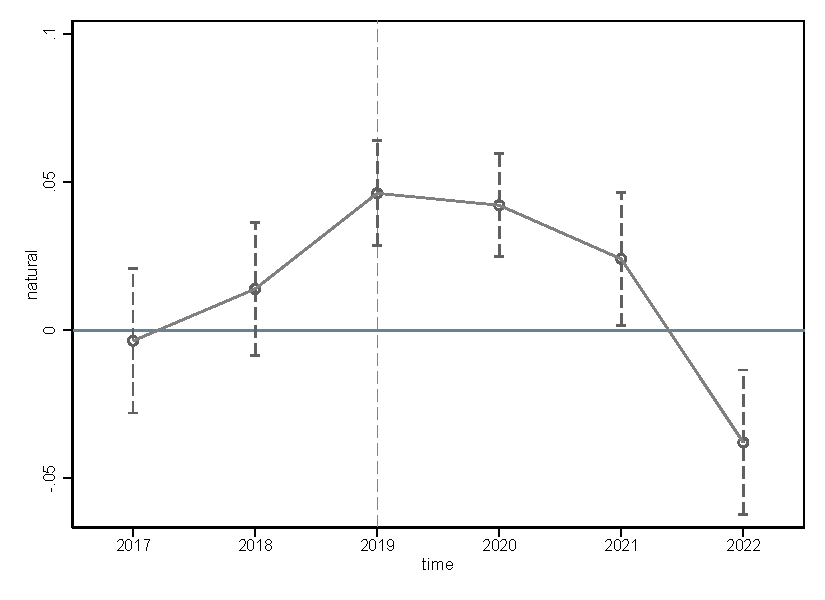
\includegraphics[width=0.5\textwidth]{../figures/did_1.pdf}\label{fig:did_num}}
    \subfloat[Effect to number of house tours]{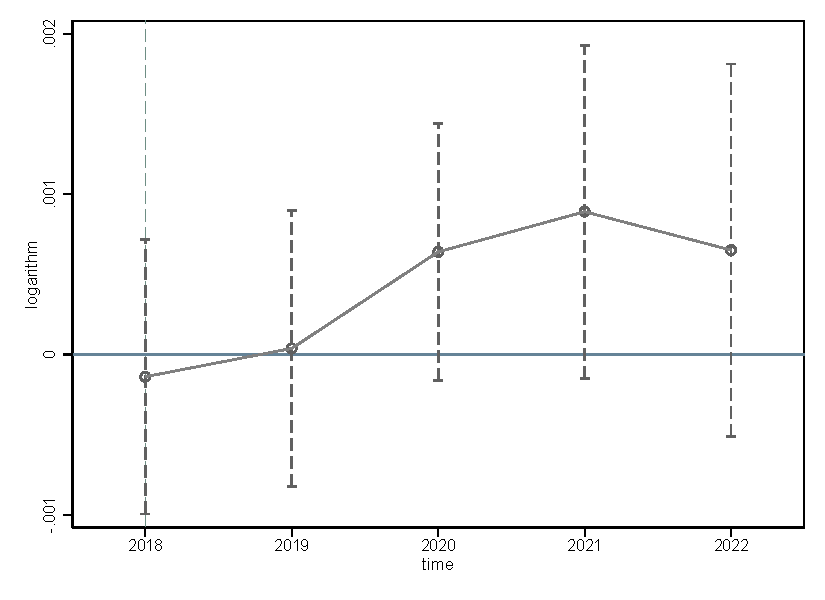
\includegraphics[width=0.5\textwidth]{../figures/did_2.pdf}\label{fig:did_lead_times}}
    \hfill % Adds horizontal space between figures
    \subfloat[Effect to transaction period]{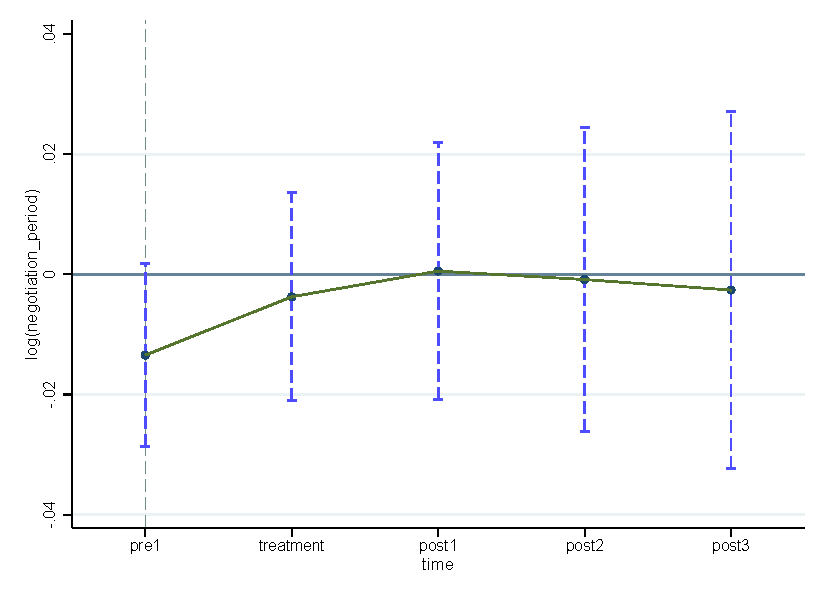
\includegraphics[width=0.5\textwidth]{../figures/did_3.pdf}\label{fig:negotiation_period}}
    \subfloat[Effect to price concession]{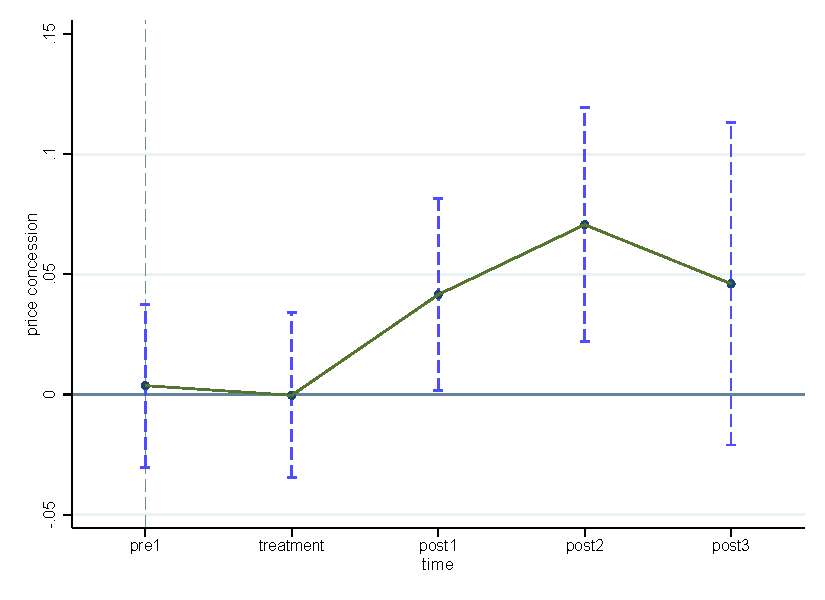
\includegraphics[width=0.5\textwidth]{../figures/did_4.pdf}\label{fig:did_price_concession}}
    \caption{Estimation of Platform Consolidation Effect}
    \label{fig:dynamic_effect}
\end{figure}

The empirical findings indicate that in the first year of the consolidation strategy, Lianjia's transaction number did not show a statistically significant difference. However, after the first year, the transaction number demonstrated a significant positive increase, ranging from 2.9\% to 6.2\%. Additionally, the platform consolidation had a significantly positive impact on the number of house tours, with effects following the same trend as the transaction revenue. Furthermore, when comparing the effect of platform consolidation with the entry effect of offline stores, the result indicates that the effect is substantially more pronounced and more continuous. These results underscore the superior efficacy of platform consolidation in enhancing market performance and provide compelling evidence for the strategic advantage of consolidation over traditional offline expansion. However, in terms of the transaction period, the consolidation strategy does not exhibit a significant effect, indicating that consolidation does not assist brokerages in facilitating better matching and negotiation between sellers and buyers. Moreover, in terms of the platform's consolidation effect on price concessions, we find that the effect is significant after the first period, with a 4.2\% increase in the first year after the treatment and a 7.1\% increase in the second year. However, the effect becomes insignificant after the third year. 

Overall, the results indicate that, compared to the offline store entry effect, the platform consolidation strategy has a more pronounced influence on both transaction effectiveness and consumer response to housing units. However, this strategy does not appear to be beneficial for sellers in the market. The benefits in terms of transaction period are not significant, and the increasing price concessions suggest that sellers are compelled to adjust listing prices to attract buyers. This can be attributed to the brokerage's increased control of information, which follows from attracting more sellers to join the network. While this provides a better match for buyers, it deteriorates the benefits for sellers. Consequently, the combined forces of better information provision for buyers and the influx of sellers keep the transaction period unchanged for houses that complete transactions, but there are more houses that fail to make a deal. It is worth noting that our data does not allow for separate estimation of these effects, which warrants further research. These findings align with the intuition that larger network effects are more likely to positively impact market performance but may not bring benefits to sellers.

% Overall, the results indicate that, compared to the offline store entry effect, the platform consolidation strategy has a more pronounced influence on both transaction effectiveness and consumer response to housing units. This can be attributed to the increased control of information by the brokerage, which enables better alignment with consumer preferences. Consequently, the brokerage can provide enhanced services tailored to individual tastes, thereby facilitating transactions more effectively. These findings align with the intuition that the larger the network effect, the more likely it is to positively impact market performance and consumer satisfaction.

To further investigate the impact of market concentration on the effectiveness of the platform consolidation strategy, we also classified the samples into low, moderate and high HHI groups and estimated the model separately for each group. The high HHI group, representing markets with higher concentration, revealed that the platform consolidation strategy does not confer significant benefits for Lianjia's operations. Conversely, in the low HHI group, indicative of less competitive markets, the consolidation strategy significantly increases the transaction number. This suggests that the platform consolidation strategy is more effective in less competitive markets, enhancing Lianjia's competitiveness. In terms of the number of house tours, the effect of platform consolidation is consistent across both high and low HHI groups. This consistency aligns with the intuition that consumer preferences for different types of brokerages are similar, and individuals are equally likely to search for houses online regardless of the brokerage's market share. Moreover, our analysis in columns 5 to 8 shows that the consolidation strategy does not have a significant effect on the transaction period or price concessions. This finding suggests that the consolidation strategy does not facilitate better matching between buyers and sellers or improve the negotiation process. This aligns with the intuition that while the consolidation strategy can attract more customers and generate revenue, it does not inherently improve the efficiency of matching buyers and sellers or negotiating terms because most of the transactions are still offline based.

\begin{table}
  \begin{center}
    \begin{scriptsize}
      \caption{Robustness Check of Online Consolidation Effect}
      \label{tab:heter_platform_did_1}
      {
\def\sym#1{\ifmmode^{#1}\else\(^{#1}\)\fi}
\begin{tabular}{l*{6}{c}}
\toprule
            &\multicolumn{1}{c}{(1)}&\multicolumn{1}{c}{(2)}&\multicolumn{1}{c}{(3)}&\multicolumn{1}{c}{(4)}&\multicolumn{1}{c}{(5)}&\multicolumn{1}{c}{(6)}\\
            &\multicolumn{1}{c}{log(income)}&\multicolumn{1}{c}{log(income)}&\multicolumn{1}{c}{log(income)}&\multicolumn{1}{c}{log(lead times)}&\multicolumn{1}{c}{log(lead times)}&\multicolumn{1}{c}{log(lead times)}\\
\midrule
pre1\_treatment&      -0.019         &      -0.012         &       0.021         &       0.017         &       0.015         &      -0.044\sym{**} \\
            &     (0.021)         &     (0.016)         &     (0.030)         &     (0.015)         &     (0.013)         &     (0.019)         \\
\addlinespace
treatment   &      -0.033\sym{*}  &      -0.002         &       0.020         &       0.006         &      -0.002         &      -0.017         \\
            &     (0.018)         &     (0.017)         &     (0.033)         &     (0.016)         &     (0.013)         &     (0.022)         \\
\addlinespace
post1\_treatment&       0.038\sym{*}  &       0.072\sym{***}&       0.051         &       0.046\sym{**} &       0.035\sym{**} &      -0.006         \\
            &     (0.022)         &     (0.019)         &     (0.036)         &     (0.018)         &     (0.014)         &     (0.024)         \\
\addlinespace
post2\_treatment&       0.059\sym{***}&       0.080\sym{***}&       0.031         &       0.040\sym{*}  &       0.028\sym{*}  &      -0.007         \\
            &     (0.023)         &     (0.021)         &     (0.041)         &     (0.021)         &     (0.016)         &     (0.024)         \\
\addlinespace
post3\_treatment&      -0.002         &       0.069\sym{***}&       0.046         &       0.027         &      -0.006         &       0.025         \\
            &     (0.026)         &     (0.025)         &     (0.070)         &     (0.023)         &     (0.019)         &     (0.028)         \\
\addlinespace
broker\_410  &      -0.001         &      -0.001         &       0.008\sym{*}  &      -0.001         &       0.002         &      -0.005         \\
            &     (0.002)         &     (0.002)         &     (0.005)         &     (0.001)         &     (0.002)         &     (0.003)         \\
\addlinespace
ln\_end\_price&       0.895\sym{***}&       0.849\sym{***}&       1.019\sym{***}&       0.181\sym{***}&       0.204\sym{***}&      -0.311\sym{***}\\
            &     (0.039)         &     (0.045)         &     (0.073)         &     (0.034)         &     (0.038)         &     (0.033)         \\
\addlinespace
ln\_watch\_people&       0.042\sym{***}&       0.046\sym{***}&       0.028\sym{***}&       0.340\sym{***}&       0.342\sym{***}&       0.366\sym{***}\\
            &     (0.006)         &     (0.006)         &     (0.009)         &     (0.008)         &     (0.007)         &     (0.004)         \\
\addlinespace
ln\_watch\_time&       0.019\sym{***}&       0.024\sym{***}&       0.034\sym{***}&       0.026\sym{***}&       0.028\sym{***}&       0.035\sym{***}\\
            &     (0.003)         &     (0.003)         &     (0.004)         &     (0.003)         &     (0.003)         &     (0.002)         \\
\addlinespace
ln\_nego\_changes&       0.023\sym{***}&       0.010         &       0.017         &       0.115\sym{***}&       0.128\sym{***}&       0.668\sym{***}\\
            &     (0.009)         &     (0.010)         &     (0.016)         &     (0.012)         &     (0.010)         &     (0.009)         \\
\addlinespace
ln\_negotiation\_period&       0.064\sym{***}&       0.075\sym{***}&       0.089\sym{***}&       0.086\sym{***}&       0.123\sym{***}&                     \\
            &     (0.005)         &     (0.005)         &     (0.010)         &     (0.006)         &     (0.006)         &                     \\
\midrule
\(N\)       &       41849         &       53806         &       24273         &       41849         &       53806         &      468936         \\
R-squared   &       0.896         &       0.902         &       0.919         &       0.935         &       0.927         &       0.528         \\
\bottomrule
\multicolumn{7}{l}{\footnotesize Standard errors in parentheses}\\
\multicolumn{7}{l}{\footnotesize \sym{*} \(p<0.1\), \sym{**} \(p<0.05\), \sym{***} \(p<0.01\)}\\
\end{tabular}
}

    
    Note: we omit all the control variables in the regression model, and detailed descriptions can be seen from Table \ref{tab:statistical_district} and Table \ref{tab:statistical_individual}. Standard Errors are clustered at the business area level.
    \end{scriptsize}
  \end{center}
\end{table}

\begin{table}
  \begin{center}
    \begin{scriptsize}
      \caption{Robustness Check of Online Consolidation Effect (Continued)}
      \label{tab:heter_platform_did_2}
      {
\def\sym#1{\ifmmode^{#1}\else\(^{#1}\)\fi}
\begin{adjustbox}{max width=\textwidth}
\begin{tabular}{l*{6}{c}}
\toprule
            &\multicolumn{1}{c}{(1)}&\multicolumn{1}{c}{(2)}&\multicolumn{1}{c}{(3)}&\multicolumn{1}{c}{(4)}&\multicolumn{1}{c}{(5)}&\multicolumn{1}{c}{(6)}\\
            &\multicolumn{1}{c}{log(negotiation period)}&\multicolumn{1}{c}{log(negotiation period)}&\multicolumn{1}{c}{log(negotiation period)}&\multicolumn{1}{c}{price concession}&\multicolumn{1}{c}{price concession}&\multicolumn{1}{c}{price concession}\\
\midrule
pre1\_treatment&       0.001         &      -0.002         &      -0.044\sym{*}  &       0.012         &      -0.011         &      -0.017         \\
            &     (0.017)         &     (0.016)         &     (0.025)         &     (0.041)         &     (0.034)         &     (0.049)         \\
\addlinespace
treatment   &       0.001         &      -0.004         &       0.014         &       0.017         &      -0.017         &      -0.019         \\
            &     (0.021)         &     (0.016)         &     (0.030)         &     (0.041)         &     (0.036)         &     (0.060)         \\
\addlinespace
post1\_treatment&       0.001         &      -0.015         &       0.005         &       0.084\sym{*}  &       0.026         &       0.020         \\
            &     (0.025)         &     (0.020)         &     (0.031)         &     (0.050)         &     (0.041)         &     (0.066)         \\
\addlinespace
post2\_treatment&      -0.002         &      -0.022         &      -0.013         &       0.160\sym{***}&       0.068         &       0.092         \\
            &     (0.027)         &     (0.023)         &     (0.029)         &     (0.056)         &     (0.048)         &     (0.077)         \\
\addlinespace
post3\_treatment&      -0.004         &      -0.011         &       0.026         &       0.034         &       0.118\sym{*}  &      -0.086         \\
            &     (0.031)         &     (0.026)         &     (0.040)         &     (0.067)         &     (0.067)         &     (0.130)         \\
\addlinespace
other brokerage num  &      -0.001         &      -0.000         &      -0.003         &      -0.008\sym{***}&      -0.001         &       0.002         \\
            &     (0.001)         &     (0.002)         &     (0.004)         &     (0.003)         &     (0.004)         &     (0.010)         \\
\addlinespace
ln(Price)&      -0.111\sym{***}&      -0.243\sym{***}&      -0.334\sym{***}&       1.246\sym{***}&       1.365\sym{***}&       1.636\sym{***}\\
            &     (0.032)         &     (0.025)         &     (0.035)         &     (0.080)         &     (0.083)         &     (0.120)         \\
\addlinespace
log(watch people)&       0.362\sym{***}&       0.368\sym{***}&       0.367\sym{***}&       0.090\sym{***}&       0.060\sym{***}&       0.037\sym{***}\\
            &     (0.005)         &     (0.004)         &     (0.005)         &     (0.006)         &     (0.006)         &     (0.007)         \\
\addlinespace
log(watch time)&       0.041\sym{***}&       0.038\sym{***}&       0.035\sym{***}&      -0.052\sym{***}&      -0.056\sym{***}&      -0.058\sym{***}\\
            &     (0.003)         &     (0.002)         &     (0.003)         &     (0.005)         &     (0.004)         &     (0.005)         \\
\addlinespace
log(nego changes)&       0.653\sym{***}&       0.663\sym{***}&       0.665\sym{***}&       0.177\sym{***}&       0.159\sym{***}&       0.173\sym{***}\\
            &     (0.008)         &     (0.007)         &     (0.010)         &     (0.009)         &     (0.008)         &     (0.011)         \\
\midrule
\(N\)       &      333284         &      587056         &      345003         &      328031         &      576728         &      338698         \\
R-squared   &       0.548         &       0.538         &       0.529         &       0.255         &       0.247         &       0.270         \\
\bottomrule
\multicolumn{7}{l}{\footnotesize Standard errors in parentheses}\\
\multicolumn{7}{l}{\footnotesize \sym{*} \(p<0.1\), \sym{**} \(p<0.05\), \sym{***} \(p<0.01\)}\\
\end{tabular}
\end{adjustbox}
}

    
    Note: we omit all the control variables in the regression model, and detailed descriptions can be seen from Table \ref{tab:statistical_district} and Table \ref{tab:statistical_individual}. Standard Errors are clustered at the business area level.
    \end{scriptsize}
  \end{center}
\end{table}

Appendix Figure \ref{fig:treatment_consolidation} illustrates the distribution of income across the treatment and control groups. Prior to the intervention, the two groups exhibit parallel trends, indicating no significant differences. The treatment effect becomes significant only after the first period, aligning with our empirical findings. 

Same as the Section \ref{subsec:entry_effect}, we performed the estimation without incorporating additional control variables, as documented in Appendix Table \ref{tab:robustness_check_platform_1} and Appendix Table \ref{tab:robustness_check_platform_2}. The findings remain consistent with our initial estimates. In the Appendix Table \ref{tab:robustness_nighttime_light_consolidation}, we also categorize the sample into areas with low and high nighttime light. The results from this stratification further corroborate the robustness of our original conclusions.

We conducted a placebo test, as illustrated in Appendix Figure \ref{fig:placebo_concession_plat} like our previous estimation of the offline store expansion. The test result also shows that there is no other confounding factors affecting our analysis. 

\section{Extension: Network Clustering Effect} \label{sec:network_effect}

\subsection{Measure of Network Effect} \label{subsec:measure_network_effect}

However, how do we measure the network effect and understand its formation? What constitutes the formation of the network effect? Previous literature illustrates that the strength of network effects and network clustering can be crucial for the operation of platforms and long-run competitiveness \citep{WOS:000454186600016}. The real estate market is characterized as a thin market, where local clustering patterns are more important in transactions, and people tend to have preferences within a given region. Therefore, segmented markets are largely independent of one another. In this context, brokerages have been fragmented into local clusters within each segmented market, allowing competitors to enter other segmented markets with relatively low costs. However, the entry barriers within markets already dominated by Lianjia are largely dependent on the network effects within these clusters. Thus, it is necessary to consider the network structure of Lianjia's offline stores and evaluate the impact of this network structure on neighborhoods within the segmented market.

We proposed a measure for the network clustering effect within the segmented market by treating offline stores and neighborhoods as nodes in a graph. Each offline store is connected to a neighborhood if the distance between them is within a five-minute walk, in line with the proposed five-minute walk strategy, and assigning a weight of $1$ if the store and neighborhood nodes are connected. To document the connections between offline stores, for each year, we calculated the shared neighborhood transaction numbers and divided this by the total transaction numbers for store $i$ and store $j$. Mathematically, this can be represented as:

\begin{equation}
  \text{weight}_{ij} = \frac{(\text{shared transactions between store $i$ and store $j$})^2}{\text{total transaction for store $i$} \times \text{total transaction in store $j$}} \label{eq:weight_between_stores}
\end{equation}

This weight represents the strength of the connection between the stores, enabling us to construct a network graph for our analysis. To visualize this network, we randomly selected 10 points and used a maximum search depth of 10 to plot the graph, as shown in Figure \ref{fig:network_formation_effect_graph}. We constructed the measure indices as local clustering effect and global clustering effect. The local clustering effect refers to the degree to which nodes in a network tend to cluster together, forming tight-knit groups. In contrast, the global clustering effect shows the overall pattern of clustering across the entire network. Detailed indices for each city and each year is reported in Table \ref{tab:local_global_clustering_indices}. In this graph, the size of the nodes indicates the significance of the local clustering effect, with larger nodes representing stronger local clustering. 

% 从图中,我们可以发现大多数的节点都是相互连接的,但是部分节点是与其他节点互不相连的,这一方面说明了,对于部分局部市场,链家拥有的网络效应并不是很强,也证明了链家的网络更类似于局部的clustering而不是整体相连;另一方面,对于最大的connected component,节点的分布也具有不对称性,可以看到部分门店具有中心作用,其拥有更大的网络可达性,而部分节点虽然与其他节点相连,但是其更多的是处于局部小三角,小聚合,所以其网络效应不大。最后,我们可以发现,对于门店节点所连接的其他neighborhood节点,其分布也不具备对称性,对于高聚合度的门店节点其拥有的neighborhood节点也更为密集,这一方面是因为其具有更高的经济价值,所以其在网络中的地位也更高,所以其拥有的网络效应也更强。最后,综合来看

From the figure, we can observe that most nodes are interconnected, but some nodes are not connected to others. This indicates that, in certain local markets, Lianjia's network effect is not very strong, demonstrating that Lianjia's network is more akin to localized clustering rather than being entirely interconnected. On the other hand, for the largest connected component, the distribution of nodes is also asymmetric. Some stores play a central role, possessing greater network accessibility, while other nodes, although connected to others, are more likely to form small local triangles or clusters, resulting in a smaller network effect. Finally, we can observe that the distribution of neighborhood nodes connected to store nodes is also asymmetrical. Stores with higher aggregation degrees have denser neighborhood nodes, partly due to their higher economic value, which enhances their status in the network and strengthens their network effect. Overall, these observations suggest that while Lianjia's network exhibits significant local clustering, its overall network connectivity varies, with certain stores and neighborhoods playing pivotal roles due to their higher economic significance. The stronger network effects observed in high-value areas emphasize the role of economic factors in shaping the structure and influence of the network.

From Table \ref{tab:local_global_clustering_indices}, we observe a general increasing trend in the network effects during the study period, with some cities exhibiting more pronounced network effects than others. However, it is important to note that no city demonstrates a particularly strong network effect throughout the research period; the network effects remain moderate. This suggests that the observed network structure is characterized by local clustering rather than extensive global connectivity, consistent with our graphical observations. Moreover, Lianjia's network effects exhibit similar patterns in terms of local clustering indices across different cities. However, the overall connectivity, as indicated by the global clustering index, varies significantly among cities. For instance, Guangzhou has a global clustering index of 0.56, indicating a very high level of overall connectivity. This contrast highlights the heterogeneous nature of network structures across different urban markets. 

\begin{figure}
  \centering
  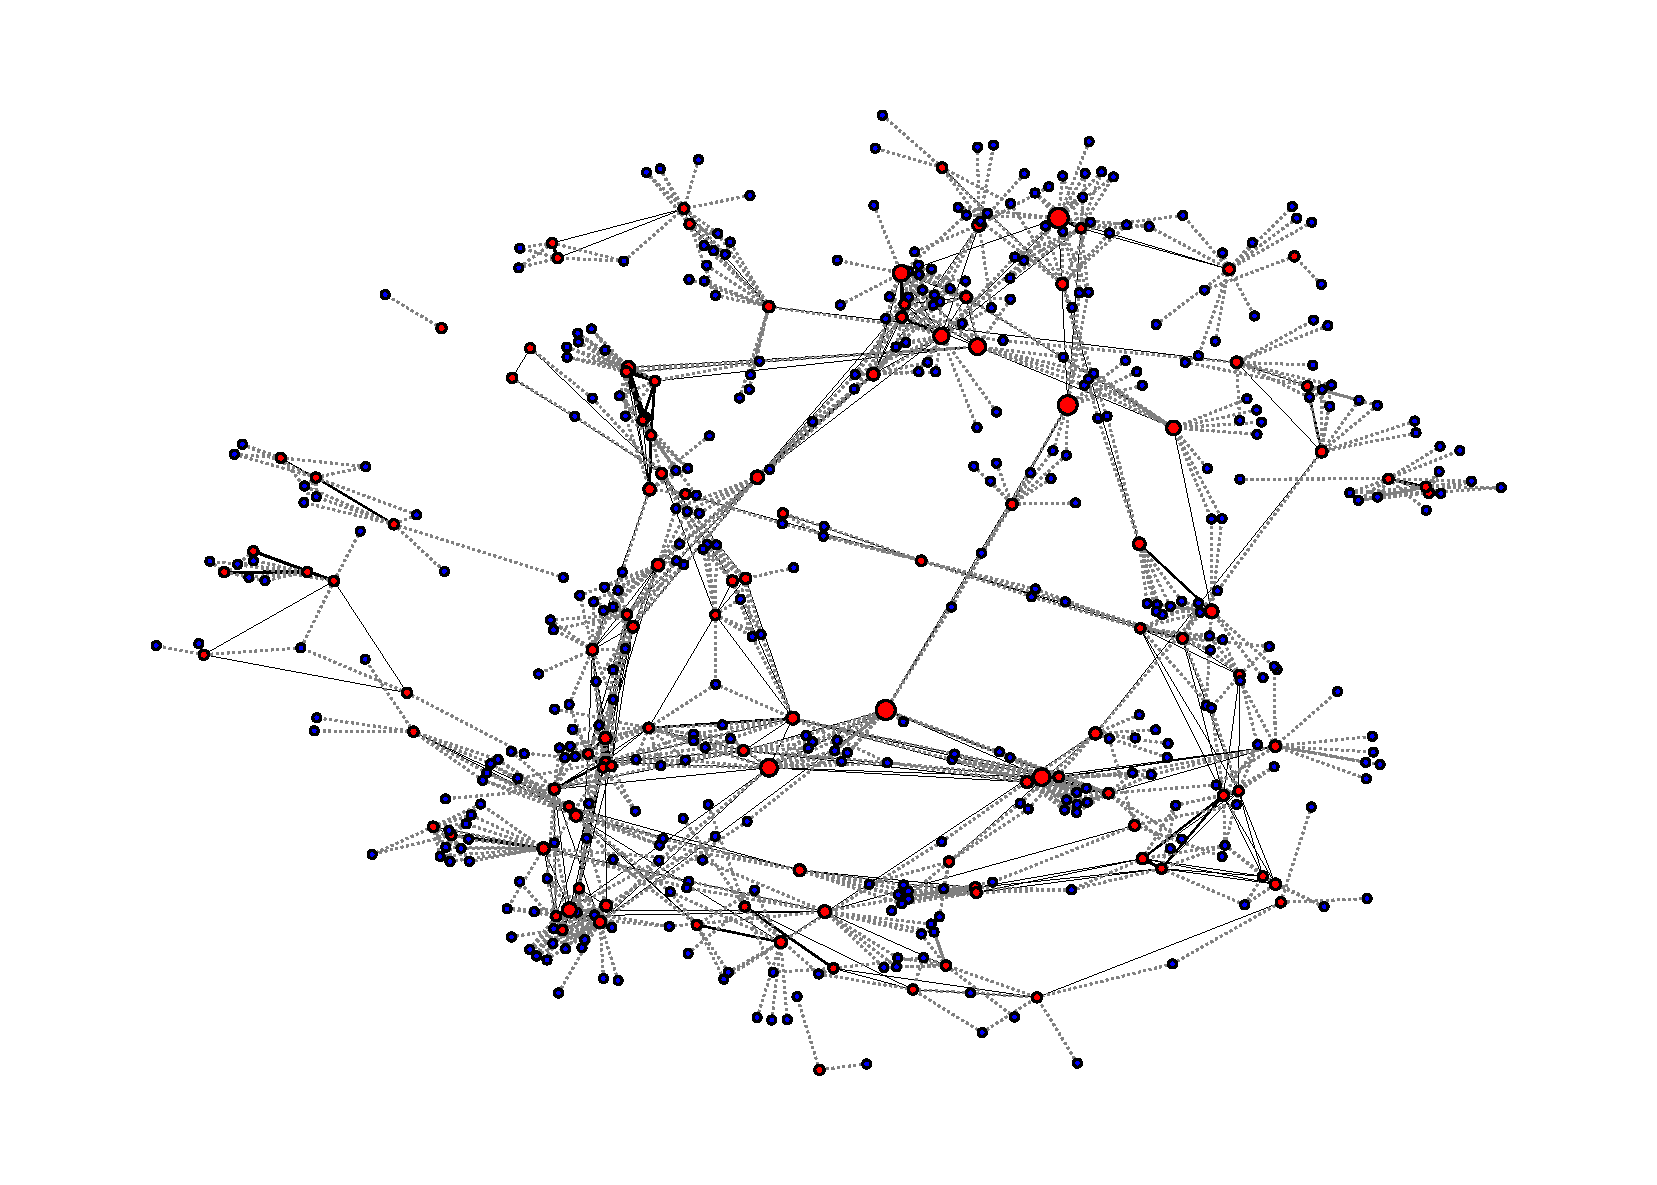
\includegraphics[width=0.7\textwidth]{../figures/network_formation_effect.pdf}
  \caption{The Structure of Network Formation Effect}
  \label{fig:network_formation_effect_graph}

  Note: The red nodes represent the distribution of Lianjia's offline stores, while the blue nodes indicate the distribution of neighborhoods within the market. Dotted edges illustrate the connections between neighborhoods and stores, whereas solid lines depict the interactions between offline stores. The size of the red nodes corresponds to the local clustering effect, with larger nodes indicating a more significant local clustering phenomenon.
\end{figure}

\begin{table}
  \begin{center}
    \begin{scriptsize}
      \caption{Average Local Clustering Index and Global Clustering Index}
      \label{tab:local_global_clustering_indices}
      \begin{tabular}{lllllllll}
\hline
 city      & index                    & 2016   & 2017   & 2018   & 2019   & 2020   & 2021    & 2022   \\
\hline
 Beijing   & average local clustering & 0.15   & 0.18   & 0.19   & 0.19   & 0.20   &         &        \\
 Beijing   & global clustering        & 0.30   & 0.36*  & 0.38*  & 0.38*  & 0.41*  &         &        \\
 Chengdu   & average local clustering & 0.20   & 0.21   & 0.20   & 0.22   & 0.23   &         &        \\
 Chengdu   & global clustering        & 0.29   & 0.29   & 0.33*  & 0.35*  & 0.38*  &         &        \\
 Chongqing & average local clustering & 0.09   & 0.13   & 0.14   & 0.16   & 0.21   & 0.23    & 0.24   \\
 Chongqing & global clustering        & 0.20   & 0.24   & 0.28   & 0.31*  & 0.44*  & 0.52**  & 0.56** \\
 Guangzhou & average local clustering & 0.06   & 0.16   & 0.17   & 0.16   & 0.24   & 0.27    & 0.28   \\
 Guangzhou & global clustering        & 0.12   & 0.33*  & 0.40*  & 0.31*  & 0.43*  & 0.53**  & 0.57** \\
 Hangzhou  & average local clustering & 0.14   & 0.16   & 0.16   & 0.18   & 0.25   & 0.25    & 0.24   \\
 Hangzhou  & global clustering        & 0.24   & 0.32*  & 0.35*  & 0.34*  & 0.46*  & 0.48*   & 0.51** \\
 Nanjing   & average local clustering & 0.16   & 0.23   & 0.23   & 0.23   & 0.25   & 0.25    & 0.25   \\
 Nanjing   & global clustering        & 0.29   & 0.42*  & 0.44*  & 0.43*  & 0.46*  & 0.48*   & 0.50*  \\
 Shanghai  & average local clustering & 0.21   & 0.21   & 0.20   & 0.21   & 0.19   & 0.18    & 0.18   \\
 Shanghai  & global clustering        & 0.35*  & 0.43*  & 0.43*  & 0.40*  & 0.33*  & 0.34*   & 0.39*  \\
 Shenzhen  & average local clustering & 0.14   & 0.22   & 0.21   & 0.18   & 0.25   &         &        \\
 Shenzhen  & global clustering        & 0.27   & 0.40*  & 0.40*  & 0.37*  & 0.49*  &         &        \\
 Tianjin   & average local clustering & 0.13   & 0.16   & 0.16   & 0.19   & 0.24   & 0.24    & 0.24   \\
 Tianjin   & global clustering        & 0.20   & 0.28   & 0.27   & 0.32*  & 0.43*  & 0.46*   & 0.47*  \\
 Wuhan     & average local clustering & 0.09   & 0.15   & 0.17   & 0.19   & 0.25   &         &        \\
 Wuhan     & global clustering        & 0.26   & 0.38*  & 0.44*  & 0.41*  & 0.55** &         &        \\
\hline
\end{tabular}

      Note: The indices used are the Average and Global Clustering Coefficients. $*$ denotes a low network effect, which ranges from 0.3 to 0.5. $**$ indicates a moderate network effect, ranging from 0.5 to 0.75. $***$ signifies a large network effect, ranging from 0.75 to 1. In the Appendix Section \ref{subsec:descriptions_clustering_indices}, we provide detailed descriptions of these indices. Moreover, Appendix Section \ref{subsec:other_indices_measures} describes other measures of network indices, including Appendix Table \ref{other:closeness_centrality}, Appendix Table \ref{other:degree_centrality} and Appendix Table \ref{other:page_rank}.
    \end{scriptsize}
  \end{center}
\end{table}

To calculate the network effect on the neighborhoods in the graph, we then calculated the network clustering effect for each neighborhood using Breadth First Search Algorithm (BFS) described in the Algorithm \ref{alg:clustering_effect}:

\begin{algorithm}[H]
  \caption{Calculate Clustering Effect for Each Neighborhood}
  \label{alg:clustering_effect}
  \begin{algorithmic}[1]
    \STATE \textbf{Input:} Graph $G = (N, E)$ with neighborhoods and stores, edge weights $w_{ij}$.
    \STATE \textbf{Output:} Clustering effect for each neighborhood.

    \FOR{each neighborhood $n \in N$}
      \STATE Initialize the set of directly connected stores $S_n$.
      \STATE Initialize queue $Q \leftarrow \{(s, w_{ns}) \mid s \in S_n\}$.
      \STATE Initialize set of visited stores $V \leftarrow \{s \mid s \in S_n\}$.
      \STATE Initialize $\text{Cluster Effect}_n \leftarrow 0$.

      \WHILE{$Q$ is not empty}
        \STATE Dequeue $(s, \text{effect}_s) \leftarrow Q.\text{pop}(0)$.
        \FOR{each neighbor store $s^\prime \in G.\text{neighbors}(s)$}
          \IF{$s^\prime \notin V$}
          \STATE Calculate propagated effect $\text{effect}_{s^\prime} \leftarrow \text{effect}_s \times w_{ss^\prime}$.
                \STATE Enqueue $(s^\prime, \text{effect}_{s^\prime})$ into $Q$.
                \STATE Add $s^\prime$ to visited set $V$.
            \ENDIF
        \ENDFOR
        \STATE Accumulate $\text{Cluster Effect}_n \leftarrow \text{Cluster Effect}_n + \text{effect}_s$.
      \ENDWHILE
    \ENDFOR
    \STATE \textbf{return} Clustering effects for all neighborhoods.
  \end{algorithmic}
\end{algorithm}

% need to refine
This approach allows us to quantify the local clustering effect within the segmented market and assess its impact on neighborhoods. The average effect of the network is 2.18 and the standard deviation is 2.55. We describe these indices in detail in Appendix Section \ref{subsec:descriptions_clustering_indices}.\footnote{We also Describes other measures of network indices in Appendix Section \ref{subsec:other_indices_measures}, including Appendix Table \ref{other:closeness_centrality}, Appendix Table \ref{other:degree_centrality} and Appendix Table \ref{other:page_rank}.} This connection is in line with the reality in several ways. Firstly, cooperation between stores to complete a transaction is very common, and having more stores within the segmented market can contribute significantly to the transaction process as more efforts can be jointly made by different agents. The collaboration between agents enhances the efficiency and effectiveness of the transaction process, leading to potentially quicker sales and better matching between buyers and properties. Secondly, the influence of the network decays with distance from subconnected nodes. This is due to the diminishing benefits of connecting with more distant nodes, as the value of information decreases with increasing distance. Information shared over longer distances may lose relevance or accuracy, thereby reducing its appeal and utility in facilitating transactions. Thirdly, we disregard each neighborhood's influence from other neighborhoods. This assumption is consistent with the observation that most houses within a neighborhood share similar characteristics, and the transaction effects within one neighborhood do not significantly impact other neighborhoods. Lastly, following Lianjia's platform consolidation strategy, the company decided to consolidate downstream brokerages to form larger clusters within the segmented market. This strategy primarily focuses on enhancing the connectivity and collaboration among stores within the network. To assess the impact of this strategy, we can examine the effects at the neighborhood level, as the increased cooperation among stores is expected to influence local market dynamics. By analyzing the neighborhood-level effects, we can better understand how the consolidation of brokerages translates into improved transaction efficiency and enhanced network effects, thereby reflecting the overall success of the platform consolidation strategy.

\subsection{Estimation of Network Consolidation on Network Effect} \label{subsec:platform_network_effect}

To empirically estimate the impact of network consolidation on the network effect, we also consider the influence of Lianjia's platform consolidation strategy on the local network clustering effect for each neighborhood. This strategy primarily targets Lianjia's offline stores, and its impact is likely to be heterogeneous across different neighborhoods. Specifically, neighborhoods that already had a diverse range of stores within the network before the strategy's implementation are expected to experience a more pronounced effect. Conversely, in neighborhoods where the local network effect was initially weak, the strategy's influence is expected to be relatively limited. 

In this context, a DID estimator can be employed to evaluate the average treatment effect. However, given the dynamic nature of the strategy's implementation across different periods, the traditional DID approach may not fully capture the varying impacts. Therefore, we employ a quantile regression estimator, as described in the model proposed by \citep{machado_quantiles_2019}, to better understand the distributional effects of the strategy. The quantile regression approach allows us to analyze the impact of the platform consolidation strategy across different points in the distribution of the local network clustering effect. This method provides a more nuanced understanding of how the strategy affects neighborhoods differently, capturing both the average treatment effect and the variability in effects across the distribution. The model is described as the follows:

\begin{equation}
  \begin{aligned}
    Q_y(\tau \mid X) & = \beta_0 + \beta_1(\tau) \text{Pre\_Treatment}_{it} + \beta_2(\tau) \text{Treatment}_{it} + \sum_{j=3}^5 \beta_j(\tau) \text{Post\_j\_Treatment}_{it} \\
                     & + \alpha(\tau) \bf{X}_{it} + \mu_i + \eta_t + \epsilon_{it}
  \end{aligned}
\end{equation}

where $Q_y(\xi \mid X)$ represents the $\tau$-th quantile of the dependent variable $y$ given the predictors $X$, where $\tau \in \{5, 10, \ldots, 95\}$. $\beta_0$ is the intercept term, $\text{Pre\_Treatment}_{it}$ is a dummy variable indicating the pre-treatment period, $\text{Treatment}_{it}$ is a dummy variable indicating the treatment group in 2018 and $\text{Post\_j\_Treatment}$ are a set of dummy variables indicating the post treatment group interacting with that year. $\mu_i$ represents individual fixed effects and $\eta_t$ is the year fixed effect and $\epsilon_{it}$ is the error term. To eliminate potential biases arising from nodes that are perpetually isolated from the network, such as neighborhoods with very few listings, we have decided to exclude samples that do not have any connections with other nodes. The results are reported in Table \ref{tab:quantile_estimate_network_1} and Table \ref{tab:quantile_estimate_network_2}. 

Table \ref{tab:quantile_estimate_network_1} and Table \ref{tab:quantile_estimate_network_2} presents the quantile estimation results of the network clustering effect following the platform consolidation strategy. Prior to the treatment, the coefficients are not significant at the 10\% level, indicating no observable effect on the network clustering effect and no observatory changes before the effect. In the first period after the platform consolidation strategy's implementation, the influence on the lowest 5\% quantile of the network is not significant at the 10\% level. However, there is a significant increase in network clustering, with a coefficient of 0.86, though the magnitude of this effect decreases as the quantile level increases. This suggests that the platform consolidation strategy has a more pronounced impact on neighborhoods with initially lower network clustering, facilitating the formation of larger and more connected networks.

The effect of the strategy continues to grow in magnitude in the first period post treatment groups, with coefficients increasing from 1.1 to 1.4 across the quantiles and this effect is also significantly larger in magnitude when compared to the mean network effect of 2.18. This trend intensifies in the second period, with even greater changes observed in network clustering, indicating an escalating impact over time. This pattern is consistent with the intuition that the platform consolidation strategy enhances network effects by forming larger clusters within the segmented market, thereby improving transaction efficiency and market competitiveness. In the final period of the study, the trend in magnitude begins to shift. The strategy's effect becomes significant for already well-connected groups rather than for those with initially low connectivity. This indicates that the consolidation strategy continues to strengthen existing networks, making well-connected neighborhoods even more integrated and efficient. Lastly, comparing with the baseline fixed effect model, we find that the quantile regression model provides a more nuanced understanding of the distributional effects of the platform consolidation strategy, capturing the varying impacts across different quantiles of the network clustering effect.

Overall, the results suggest that the platform consolidation strategy has a significant and dynamic impact on the network clustering effect. Initially, it benefits neighborhoods with lower connectivity, helping them to form larger and more efficient clusters. Over time, the strategy's influence extends to enhance the clustering of already well-connected neighborhoods, thereby continuously improving the overall network structure and market performance. Moreover, from the long-term perspectives, the online consolidation effect is beneficial for Lianjia's competitiveness because the larger the local network effect, the better Lianjia can better can have better contorl in the information. Moreover, from a long-term perspective, the online consolidation effect enhances Lianjia's competitiveness, as a stronger local network effect enables Lianjia to exert greater control over information.

\begin{table}
  \begin{center}
    \begin{scriptsize}
      \caption{Quantile Estimation of the Network Spillover Effect}
      \label{tab:quantile_estimate_network_1}
      {
\def\sym#1{\ifmmode^{#1}\else\(^{#1}\)\fi}
\begin{tabular}{l*{10}{c}}
\toprule
            &\multicolumn{1}{c}{(1)}&\multicolumn{1}{c}{(2)}&\multicolumn{1}{c}{(3)}&\multicolumn{1}{c}{(4)}&\multicolumn{1}{c}{(5)}&\multicolumn{1}{c}{(6)}&\multicolumn{1}{c}{(7)}&\multicolumn{1}{c}{(8)}&\multicolumn{1}{c}{(9)}&\multicolumn{1}{c}{(10)}\\
            &\multicolumn{1}{c}{FE}&\multicolumn{1}{c}{Q(5)}&\multicolumn{1}{c}{Q(10)}&\multicolumn{1}{c}{Q(15)}&\multicolumn{1}{c}{Q(20)}&\multicolumn{1}{c}{Q(25)}&\multicolumn{1}{c}{Q(30)}&\multicolumn{1}{c}{Q(35)}&\multicolumn{1}{c}{Q(40)}&\multicolumn{1}{c}{Q(45)}\\
\midrule
pre1\_treatment&      -0.063\sym{*}  &       0.034         &       0.017         &       0.005         &      -0.003         &      -0.009         &      -0.017         &      -0.026         &      -0.037         &      -0.049         \\
            &     (0.033)         &     (0.584)         &     (0.518)         &     (0.473)         &     (0.441)         &     (0.416)         &     (0.388)         &     (0.352)         &     (0.312)         &     (0.267)         \\
\addlinespace
treatment   &       0.777\sym{***}&       0.878         &       0.860\sym{*}  &       0.848\sym{*}  &       0.840\sym{**} &       0.833\sym{**} &       0.826\sym{**} &       0.816\sym{**} &       0.805\sym{***}&       0.793\sym{***}\\
            &     (0.049)         &     (0.553)         &     (0.491)         &     (0.448)         &     (0.417)         &     (0.394)         &     (0.368)         &     (0.333)         &     (0.295)         &     (0.252)         \\
\addlinespace
post1\_treatment&       1.230\sym{***}&       1.433\sym{**} &       1.398\sym{**} &       1.373\sym{***}&       1.356\sym{***}&       1.343\sym{***}&       1.328\sym{***}&       1.308\sym{***}&       1.286\sym{***}&       1.261\sym{***}\\
            &     (0.068)         &     (0.650)         &     (0.577)         &     (0.527)         &     (0.491)         &     (0.463)         &     (0.432)         &     (0.392)         &     (0.347)         &     (0.297)         \\
\addlinespace
post2\_treatment&       1.618\sym{***}&       1.626\sym{**} &       1.625\sym{**} &       1.624\sym{**} &       1.623\sym{***}&       1.622\sym{***}&       1.622\sym{***}&       1.621\sym{***}&       1.620\sym{***}&       1.619\sym{***}\\
            &     (0.088)         &     (0.802)         &     (0.712)         &     (0.650)         &     (0.605)         &     (0.572)         &     (0.533)         &     (0.483)         &     (0.428)         &     (0.366)         \\
\addlinespace
post3\_treatment&       1.731\sym{***}&       1.689         &       1.697         &       1.702         &       1.705\sym{*}  &       1.708\sym{*}  &       1.711\sym{**} &       1.715\sym{**} &       1.720\sym{**} &       1.725\sym{***}\\
            &     (0.123)         &     (1.281)         &     (1.137)         &     (1.039)         &     (0.967)         &     (0.913)         &     (0.852)         &     (0.772)         &     (0.684)         &     (0.585)         \\
\addlinespace
Brokerage Control &  \checkmark         &  \checkmark         &  \checkmark         &  \checkmark         &  \checkmark         &  \checkmark         &  \checkmark         &  \checkmark         &  \checkmark         &  \checkmark         \\
\addlinespace
Hedonic Control &  \checkmark         &  \checkmark         &  \checkmark         &  \checkmark         &  \checkmark         &  \checkmark         &  \checkmark         &  \checkmark         &  \checkmark         &  \checkmark         \\
\addlinespace
Transaction Control &  \checkmark         &  \checkmark         &  \checkmark         &  \checkmark         &  \checkmark         &  \checkmark         &  \checkmark         &  \checkmark         &  \checkmark         &  \checkmark         \\
\addlinespace
Regional Control &  \checkmark         &  \checkmark         &  \checkmark         &  \checkmark         &  \checkmark         &  \checkmark         &  \checkmark         &  \checkmark         &  \checkmark         &  \checkmark         \\
\midrule
\(N\)       &      133818         &      142734         &      142734         &      142734         &      142734         &      142734         &      142734         &      142734         &      142734         &      142734         \\
\bottomrule
\multicolumn{11}{l}{\footnotesize Standard errors in parentheses}\\
\multicolumn{11}{l}{\footnotesize \sym{*} \(p<0.1\), \sym{**} \(p<0.05\), \sym{***} \(p<0.01\)}\\
\end{tabular}
}

    
    Note: we omit all the control variables in the regression model, and detailed descriptions can be seen from Table \ref{tab:statistical_district} and Table \ref{tab:statistical_individual}. Robsut Standard Errors are reported in parentheses.
    \end{scriptsize}
  \end{center}
\end{table}

\begin{table}
  \begin{center}
    \begin{scriptsize}
      \caption{Quantile Estimation of the Network Spillover Effect (Continued)}
      \label{tab:quantile_estimate_network_2}
      {
\def\sym#1{\ifmmode^{#1}\else\(^{#1}\)\fi}
\begin{tabular}{l*{10}{c}}
\toprule
            &\multicolumn{1}{c}{(1)}&\multicolumn{1}{c}{(2)}&\multicolumn{1}{c}{(3)}&\multicolumn{1}{c}{(4)}&\multicolumn{1}{c}{(5)}&\multicolumn{1}{c}{(6)}&\multicolumn{1}{c}{(7)}&\multicolumn{1}{c}{(8)}&\multicolumn{1}{c}{(9)}&\multicolumn{1}{c}{(10)}\\
            &\multicolumn{1}{c}{Q(50)}&\multicolumn{1}{c}{Q(55)}&\multicolumn{1}{c}{Q(60)}&\multicolumn{1}{c}{Q(65)}&\multicolumn{1}{c}{Q(70)}&\multicolumn{1}{c}{Q(75)}&\multicolumn{1}{c}{Q(80)}&\multicolumn{1}{c}{Q(85)}&\multicolumn{1}{c}{Q(90)}&\multicolumn{1}{c}{Q(95)}\\
\midrule
pre1\_treatment&      -0.062         &      -0.076         &      -0.089         &      -0.101         &      -0.111         &      -0.119         &      -0.127         &      -0.139         &      -0.153         &      -0.173         \\
            &     (0.216)         &     (0.166)         &     (0.124)         &     (0.092)         &     (0.078)         &     (0.080)         &     (0.095)         &     (0.128)         &     (0.173)         &     (0.247)         \\
\addlinespace
treatment   &       0.779\sym{***}&       0.764\sym{***}&       0.751\sym{***}&       0.739\sym{***}&       0.728\sym{***}&       0.720\sym{***}&       0.711\sym{***}&       0.699\sym{***}&       0.685\sym{***}&       0.664\sym{***}\\
            &     (0.205)         &     (0.157)         &     (0.117)         &     (0.087)         &     (0.073)         &     (0.076)         &     (0.090)         &     (0.121)         &     (0.164)         &     (0.233)         \\
\addlinespace
post1\_treatment&       1.233\sym{***}&       1.204\sym{***}&       1.177\sym{***}&       1.152\sym{***}&       1.129\sym{***}&       1.114\sym{***}&       1.096\sym{***}&       1.071\sym{***}&       1.044\sym{***}&       1.001\sym{***}\\
            &     (0.240)         &     (0.185)         &     (0.138)         &     (0.102)         &     (0.086)         &     (0.090)         &     (0.106)         &     (0.142)         &     (0.192)         &     (0.274)         \\
\addlinespace
post2\_treatment&       1.618\sym{***}&       1.617\sym{***}&       1.616\sym{***}&       1.615\sym{***}&       1.614\sym{***}&       1.613\sym{***}&       1.613\sym{***}&       1.612\sym{***}&       1.610\sym{***}&       1.609\sym{***}\\
            &     (0.297)         &     (0.228)         &     (0.170)         &     (0.126)         &     (0.106)         &     (0.110)         &     (0.130)         &     (0.175)         &     (0.237)         &     (0.338)         \\
\addlinespace
post3\_treatment&       1.731\sym{***}&       1.737\sym{***}&       1.742\sym{***}&       1.747\sym{***}&       1.752\sym{***}&       1.755\sym{***}&       1.759\sym{***}&       1.764\sym{***}&       1.770\sym{***}&       1.779\sym{***}\\
            &     (0.474)         &     (0.365)         &     (0.271)         &     (0.202)         &     (0.170)         &     (0.176)         &     (0.208)         &     (0.280)         &     (0.379)         &     (0.541)         \\
\addlinespace
Brokerage Control &  \checkmark         &  \checkmark         &  \checkmark         &  \checkmark         &  \checkmark         &  \checkmark         &  \checkmark         &  \checkmark         &  \checkmark         &  \checkmark         \\
\addlinespace
Hedonic Control &  \checkmark         &  \checkmark         &  \checkmark         &  \checkmark         &  \checkmark         &  \checkmark         &  \checkmark         &  \checkmark         &  \checkmark         &  \checkmark         \\
\addlinespace
Transaction Control &  \checkmark         &  \checkmark         &  \checkmark         &  \checkmark         &  \checkmark         &  \checkmark         &  \checkmark         &  \checkmark         &  \checkmark         &  \checkmark         \\
\addlinespace
Regional Control &  \checkmark         &  \checkmark         &  \checkmark         &  \checkmark         &  \checkmark         &  \checkmark         &  \checkmark         &  \checkmark         &  \checkmark         &  \checkmark         \\
\midrule
\(N\)       &      142734         &      142734         &      142734         &      142734         &      142734         &      142734         &      142734         &      142734         &      142734         &      142734         \\
\bottomrule
\multicolumn{11}{l}{\footnotesize Standard errors in parentheses}\\
\multicolumn{11}{l}{\footnotesize \sym{*} \(p<0.1\), \sym{**} \(p<0.05\), \sym{***} \(p<0.01\)}\\
\end{tabular}
}

    
    Note: we omit all the control variables in the regression model, and detailed descriptions can be seen from Table \ref{tab:statistical_district} and Table \ref{tab:statistical_individual}.
    \end{scriptsize}
  \end{center}
\end{table}

\subsection{Mechanism Design} \label{subsec:mechanism_network_design}

In the real estate market, real estate is not a homogeneous good, and therefore, the brokerage market is characterized by a large number of firms with no significant barriers to entry. Traditional economic theory suggests that such a market, characterized by substantial competition, numerous firms, and low market concentration, is consistent with real-world observations. For example, Lianjia's offline stores account for less than 5\% of the total, yet Lianjia handles about 20\% of the national transactions. In addition, many well-known agencies, such as Woaiwojia and Centaline Property Agency, operate in this market, indicating a monopolistic competitive environment.

However, when looking at local segmented markets, the monopolistic competition model seems less applicable. In local markets, surrounding neighborhoods share similar community characteristics and public resources. Especially in China's real estate market, most properties are apartments, where the inherent differences between properties are minimal, making them relatively homogeneous goods. In addition, local real estate markets have no barriers to entry or exit, closely resembling perfect competition. From a cost perspective, the real estate market has undergone platform mediated reforms, where data resources have zero marginal cost characteristics and operating costs decrease as the user base expands, suggesting characteristics of a natural monopoly. Under these conditions, the operating position of firms differs significantly from that in a monopolistically competitive market. Due to network effects, an increase in the number of branches of a dominant real estate agency attracts more users, which in turn attracts more real estate listings. This positive feedback loop reinforces the dominant position of firms like Lianjia, leading to the formation of oligopolistic firms. These oligopolistic firms can further maintain their dominant market positions.

In local segmented markets, oligopolistic firms are responsible for increasing network strength and have significant market power. In segmented markets where some oligopolistic firms do not have strong network effects, multiple other firms serve the diverse needs of consumers and expand their scale. The environment of free entry, rapid technological progress, and business model innovation leads to an inclusive competitive landscape in the real estate brokerage market. This environment allows oligopolistic firms to either enhance the strength of their network effects or have their dominant positions challenged. As a result, monopolistic structures emerge from and are subsequently disrupted by competition, allowing real estate intermediaries to continuously evolve and drive the industry's rapid growth. The practical implication is that a competitive oligopolistic structure does not inherently impede competitive efficiency. Instead, as our empirical findings indicate, the enriched entry and transformations within the market lead to an increase in the number of transactions and house tours. This type of market structure can enhance firm efficiency, thereby facilitating more efficient transactions for buyers and sellers and improving overall market welfare, even though it may impede individual seller welfare.

As our empirical results show, Lianjia's strategy has significantly enhanced its network strength within segmented markets. From this perspective, the enhancement of network effects further drives the segmented market toward an oligopolistic competitive structure, which could increase the market welfare and facilitate the transactions between buyers and sellers. Moreover, with the development of online platforms and new technologies, such as Lianjia's latest VR home viewing technology, these network effects are gradually shifting from local networks to a global network. As a result, this development is shaping the overall market into an oligopolistic competition model on a larger scale.

In the future, as the network effects intensify, the real estate brokerage market may witness a more pronounced consolidation of market power among a few dominant players. This consolidation can lead to increased efficiencies through economies of scale and scope, where firms leverage their vast data resources and technological advancements to optimize operations and enhance consumer experiences. However, this shift also raises important considerations for regulatory bodies to ensure that the market remains competitive and accessible. The dynamic interplay between technological innovation and market structure will be crucial. As firms like Lianjia continue to innovate, incorporating artificial intelligence, big data analytics, and blockchain for secure transactions, the real estate market could become more transparent and efficient. These advancements could lower transaction costs, reduce information asymmetry, and provide consumers with more personalized services. Furthermore, the global reach of network effects implies that real estate brokerage markets across different regions might become more interconnected. This interconnectivity can facilitate cross-city or cross-province investments and diversify property portfolios for investors, contributing to a more resilient real estate market.

In conclusion, the evolution of the real estate brokerage market towards an oligopolistic competition model, driven by network effects and technological advancements, presents both opportunities and challenges. From our empirical findings, this type of market structure can not impede the competitive efficiencies but policymakers and industry stakeholders must navigate this landscape carefully to harness the benefits of increased efficiency and innovation while safeguarding against potential market power abuses and ensuring equitable access for all participants. This balanced approach will be essential for sustaining long-term growth and enhancing overall market welfare in the real estate industry.

\section{Discussion and Conclusion} \label{sec:conclusion}

Our study highlights the transformative impact of Lianjia's strategic expansion in China's real estate brokerage industry through the implementation of the online-mediated consolidation strategy and the massive expansion of offline branches. Our empirical research demonstrates that Lianjia's approach, which seamlessly integrates online platforms with an extensive offline presence, significantly enhances revenue generation and influences consumer behavior through improved price concessions and increased number of house tours. Specifically, our results indicate that the expansion of Lianjia's stores leads to an increase in the company's market share in the region by 4.8\% to 9.1\% and attracts more clients, as evidenced by an increase in number of house tours by 2.3\% to 3.1\%. Additionally, the study reveals that while offline store expansion does not significantly affect the transaction period, but it facilitates better communication between buyers and sellers by contributing the price concession in transaction. Secondly, Lianjia's platform-mediated consolidation can also increase its transaction revenue by 2.9\% to 6.2\% and boost the number of house tours by 2.9\% to 3.0\%. However, this effect does not significantly influence communication, thereby not affecting price concessions or the transaction period. Lastly, we established the presence of localized network effects and found that Lianjia's network effects are primarily characterized by local clustering, with moderate network strength. The platform-mediated consolidation helps Lianjia achieve greater localized network effects, which in turn, enhances its long-term influence in the market.

Our research has several implications. Firstly, it indicates that with the advent of new technologies, the online consolidation effect is becoming increasingly important for real estate companies. This shift underscores the need for firms to enhance their digital strategies to remain competitive. Secondly, our findings have broader significance for other industries where online consolidation can potentially replace traditional offline clustering. For example, in the retail sector, online marketplaces such as Alibaba in China have significantly outpaced physical stores by consolidating various vendors into a single, accessible platform. Thirdly, this study demonstrates that, under the platform's consolidation effect, offline stores can enhance revenue and improve transaction efficiency. These findings can be extended to other similar fields, as discussed by \citep{10.1257/jep.28.2.3}. Lastly, this study also confirms that local network effect can not preclude other competitors from entering the market but the network effect can help the company to coexist with other competitors, and improve the overall market efficiency, consistent with the work by \citep{gilbukh_goldsmith-pinkham_2019}.

By examining these dynamics, our research contributes to a deeper understanding of the evolving landscape of real estate brokerage in China. It provides valuable insights for policymakers and industry stakeholders aiming to enhance market efficiency and competitiveness. As the online consolidation effect continues to grow, our findings highlight the importance of adapting to this trend and evolving strategies accordingly. Specifically, transitioning from a bilateral brokerage model to a model where buyer and seller agencies are separated could be crucial for sustaining a competitive advantage in the real estate brokerage market. This strategic shift entails leveraging online platforms to integrate services and enhance transaction efficiency, thereby benefiting both consumers and firms. By disentangling the roles of buyer and seller agents, the market can reduce conflicts of interest, increase transparency, and improve overall market efficiency. This alignment with economic principles of specialization and efficiency further underscores the potential for significant gains in consumer welfare and firm profitability.

Future research could explore several potential directions. First, investigating the long-term impacts of online and offline integration on market competition and consumer behavior in various real estate markets globally could provide comparative insights. Second, examining the role of emerging technologies, such as artificial intelligence and blockchain, in further enhancing the efficiency and transparency of real estate transactions would be valuable. Third, assessing the socio-economic implications of platform monopolization, particularly in terms of access to affordable housing and regional economic disparities, could offer important policy implications. Lastly, exploring the adaptability of the online-offline integration model in other sectors, such as healthcare and education, could extend the applicability of these findings and contribute to a broader understanding of digital transformation across industries.

% main structure:
% 1. conclusions
% 2. why the exercise is important
% 3. policy implications
% 4. further research directions

%%%%%%%%%%%%%%%%%%%%%%%%%%%%%%%%%%%%%%%%%%%%%%%%%
\clearpage
\begin{singlespace}
%\bibliographystyle{plainnat}
%\bibliographystyle{chicago}
% \bibliographystyle{aer}
% \bibliography{our-cites.bib}

\begin{thebibliography}{}
  \bibitem[Agarwal et al.(2019)]{AGARWAL2019715}
Agarwal S, He J, Sing TF, Song C (2019) Do real estate agents have information advantages in housing markets? \textit{Journal of Financial Economics} 134(3):715-735.

\bibitem[Agarwal et al.(2024)]{AGARWAL2024103668}
Agarwal S, Kuang W, Wang L, Yang Y (2024) The role of agents in fraudulent activities: Evidence from the housing market in Beijing. \textit{Journal of Urban Economics} 142:103668.

\bibitem[Akerlof(1970)]{Akerlof_1970}
Akerlof GA (1970) The Market for “Lemons”: Quality Uncertainty and the Market Mechanism. \textit{The Quarterly Journal of Economics} 84(3):488.

\bibitem[Allen et al.(2023)]{RePEc:kap:jrefec:v:67:y:2023:i:3:d:10.1007_s11146-021-09858-w}
Allen MT, Benefield JD, Rutherford RC (2023) Co-Listing Strategies: Better Transaction Outcomes? \textit{The Journal of Real Estate Finance and Economics} 67(3):517-544.

\bibitem[Armstrong(2006)]{Armstrong2006}
Armstrong M (2006) Competition in two-sided markets. \textit{The RAND Journal of Economics} 37(3):668-691.

\bibitem[Athey and Imbens(2006)]{https://doi.org/10.1111/j.1468-0262.2006.00668.x}
Athey S, Imbens GW (2006) Identification and Inference in Nonlinear Difference-in-Differences Models. \textit{Econometrica} 74(2):431-497.

\bibitem[Athey and Imbens(2016)]{athey_recursive_2016}
Athey S, Imbens GW (2016) Recursive partitioning for heterogeneous causal effects. \textit{Proceedings of the National Academy of Sciences} 113(27):7353-7360.

\bibitem[Azmi et al.(2012)]{AZMI2012406}
Azmi DI, Karim HA, Amin MZM (2012) Comparing the Walking Behaviour between Urban and Rural Residents. \textit{Procedia - Social and Behavioral Sciences} 68:406-416.

\bibitem[Bailey et al.(2018)]{bailey_economic_2018}
Bailey M, Cao R, Kuchler T, Stroebel J (2018) The Economic Effects of Social Networks: Evidence from the Housing Market. \textit{Journal of Political Economy} 126(6):2224-2276.

\bibitem[Barwick and Pathak(2015)]{https://doi.org/10.1111/1756-2171.12082}
Barwick PJ, Pathak PA (2015) The costs of free entry: an empirical study of real estate agents in Greater Boston. \textit{The RAND Journal of Economics} 46(1):103-145.

\bibitem[Barwick et al.(2017)]{10.1257/app.20160214}
Barwick PJ, Pathak PA, Wong M (2017) Conflicts of Interest and Steering in Residential Brokerage. \textit{American Economic Journal Applied Economics} 9(3):191-222.

\bibitem[Beck et al.(2022)]{doi:10.1080/10527001.2021.2016340}
Beck J, Scott F, Yelowitz A (2022) The Impact of Real Estate Agent Specialization and Activity Level on Market Outcomes. \textit{Journal of Housing Research} 31(2):163-180.

\bibitem[Chen and Wen(2017)]{chen_great_2017}
Chen K, Wen Y (2017) The Great Housing Boom of China. \textit{American Economic Journal Macroeconomics} 9(2):73-114.

\bibitem[Christensen and Timmins(2022)]{RePEc:ucp:jpolec:doi:10.1086/720140}
Christensen P, Timmins C (2022) Sorting or Steering: The Effects of Housing Discrimination on Neighborhood Choice. \textit{Journal of Political Economy} 130(8):2110-2163.

\bibitem[Chu et al.(2021)]{doi:10.1287/mnsc.2019.3550}
Chu J, Duan Y, Yang X, Wang L (2021) The Last Mile Matters: Impact of Dockless Bike Sharing on Subway Housing Price Premium. \textit{Management Science} 67(1):297-316.

\bibitem[d'Aspremont et al.(1979)]{daspremont_hotellings_1979}
D'Aspremont C, Gabszewicz JJ, Thisse J f. (1979) On Hotelling's “Stability in Competition.” \textit{Econometrica} 47(5):1145-1150.

\bibitem[Elvidge et al.(2021)]{elvidge_annual_2021}
Elvidge CD, Zhizhin M, Ghosh T, Hsu FC, Taneja J (2021) Annual Time Series of Global VIIRS Nighttime Lights Derived from Monthly Averages: 2012 to 2019. \textit{Remote Sensing} 13(5):922.

\bibitem[Farrell and Shapiro(1990)]{farrell_horizontal_1990}
Farrell J, Shapiro C (1990) Horizontal Mergers: An Equilibrium Analysis. \textit{American Economic Review} 80(1):107-126.

\bibitem[Genesove and Han(2012)]{GENESOVE201231}
Genesove D, Han L (2012) Search and matching in the housing market. \textit{Journal of Urban Economics} 72(1):31-45.

\bibitem[Gilbukh and Goldsmith-Pinkham(2019)]{gilbukh_goldsmith-pinkham_2019}
Gilbukh S, Goldsmith-Pinkham P (2019) Heterogeneous Real Estate Agents and the Housing Cycle. \textit{SSRN Electronic Journal}.

\bibitem[Glaeser et al.(2017)]{glaeser_real_2017}
Glaeser E, Huang W, Ma Y, Shleifer A (2017) A Real Estate Boom with Chinese Characteristics. \textit{The Journal of Economic Perspectives} 31(1):93-116.

\bibitem[Grossman and Stiglitz(1980)]{grossman_impossibility_1980}
Grossman SJ, Stiglitz JE (1980) On the impossibility of informationally efficient markets. \textit{American Economic Review} 70(3):393-408.

\bibitem[Han and Hong(2011)]{550a6ccf-cde2-3dd1-979f-1a8db2b8ceb9}
Han L, Hong SH (2011) Testing Cost Inefficiency Under Free Entry in the Real Estate Brokerage Industry. \textit{Journal of Business \& Economic Statistics} 29(4):564-578.

\bibitem[Han and Strange(2015)]{HAN2015813}
Han L, Strange WC (2015) The Microstructure of Housing Markets. \textit{Handbook of Regional and Urban Economics}. 813-886.

\bibitem[Handbury(2021)]{handbury_are_2021}
Handbury J (2021) Are Poor Cities Cheap for Everyone? Non-Homotheticity and the Cost of Living Across U.S. Cities. \textit{Econometrica} 89(6):2679-2715.

\bibitem[Hendel et al.(2009)]{hendel_relative_2009} 
Hendel I, Nevo A, Ortalo-Magné F (2009) The Relative Performance of Real Estate Marketing Platforms: MLS versus FSBOMadison.com. \textit{American Economic Review} 99(5):1878-1898.

\bibitem[Hong(2022)]{https://doi.org/10.1002/jae.2891}
Hong S-H (2022) Real estate agents' influence on housing search. \textit{Journal of Applied Econometrics} 37(3):563-582.

\bibitem[Hotelling(1929)]{hotelling_stability_1929}
Hotelling H (1929) Stability in Competition. \textit{The Economic Journal} 39(153):41-57.

\bibitem[Hsieh and Moretti(2003)]{hsieh_can_2003}
Hsieh C-T, Moretti E (2003) Can Free Entry Be Inefficient? Fixed Commissions and Social Waste in the Real Estate Industry. \textit{Journal of Political Economy} 111(5):1076-1122.

\bibitem[Hui and Chan(2014)]{hui_foreign_2014}
Hui ECM, Chan KKK (2014) Foreign direct investment in China's real estate market. \textit{Habitat International} 43:231-239.

\bibitem[Jud et al.(1996)]{doi:10.1080/10835547.1996.12090852}
Jud D, Seaks T, Winkler D (1996) Time on the Market: The Impact of Residential Brokerage. \textit{Journal of Real Estate Research} 12(2):447-458.

\bibitem[Langley and Leyshon(2017)]{Langley_Leyshon_2017}
Langley P, Leyshon A (2017) Platform capitalism: The intermediation and capitalisation of digital economic circulation. \textit{Finance and Society} 3(1):11-31.

\bibitem[Levitt and Syverson(2008)]{d082a2db-5cce-33f2-87c4-9cb020cc6666}
Levitt SD, Syverson C (2008) Market Distortions When Agents Are Better Informed: The Value of Information in Real Estate Transactions. \textit{The Review of Economics and Statistics} 90(4):599-611.

\bibitem[Li et al.(2019)]{LI2019165}
Li H, Wei YD, Wu Y, Tian G (2019) Analyzing housing prices in Shanghai with open data: Amenity, accessibility and urban structure. \textit{Cities} 91:165-179.

\bibitem[Li and Qi(2022)]{10.1093/cje/beac054}
Li Z, Qi H (2022) Platform power: monopolisation and financialisation in the era of big tech. \textit{Cambridge Journal of Economics} 46(6):1289-1314.

\bibitem[Liu et al.(2023)]{liu2023chrono-urbanism}
Liu D, Kwan M-P, Wang L, Kan Z, Wang J, Huang J (2024) Development of a Chrono-Urbanism Status Composite Index under the 5/10/15-Minute City Concept Using Social Media Big Data. \textit{Tijdschrift Voor Economische En Sociale Geografie}.

\bibitem[Machado and Santos Silva(2019)]{machado_quantiles_2019}
Machado JAF, Silva JMCS (2019) Quantiles via moments. \textit{Journal of Econometrics} 213(1):145-173.


\bibitem[McCrary(2008)]{MCCRARY2008698}
McCrary J (2008) Manipulation of the running variable in the regression discontinuity design: A density test. \textit{Journal of Econometrics} 142(2):698-714.

\bibitem[MOHURD(2018)]{GB50180-2018}
Ministry of Housing and Urban-Rural Development of China. 2018. Urban residential area planning and design standard (GB50180-2018). Available at: \url{http://www.moe.gov.cn/jyb_xwfb/xw_zt/moe_357/jyzt_2019n/2019_zt13/zcwj/201906/t20190606_384732.html} (accessed July 7, 2023). (in Chinese).

\bibitem[Peng(2023)]{peng_mortgage_2023}
Peng Y (2023) Mortgage Credit and Housing Markets. \textit{SSRN Electronic Journal}. % Available at \url{https://ssrn.com/abstract=4537500} or \url{http://dx.doi.org/10.2139/ssrn.4537500}. 

\bibitem[Piazzesi et al.(2020)]{10.1257/aer.20141772}
Piazzesi M, Schneider M, Stroebel J (2020) Segmented Housing Search. \textit{American Economic Review} 110(3):720-759.

\bibitem[Pope et al.(2015)]{POPE201589}
Pope DG, Pope JC, Sydnor JR (2015) Focal points and bargaining in housing markets. \textit{Games and Economic Behavior} 93:89-107.

\bibitem[Qu et al.(2021)]{qu_identifying_2021}
Qu W, Huang Y, Deng G (2021) Identifying the critical factors behind the second-hand housing price concession: Empirical evidence from China. \textit{Habitat International} 117:102442.

\bibitem[Rochet and Tirole(2003)]{10.1162/154247603322493212}
Rochet JC, Tirole J (2003) Platform Competition in Two-Sided Markets. \textit{Journal of the European Economic Association} 1(4):990-1029.

\bibitem[Rochet and Tirole(2006)]{https://doi.org/10.1111/j.1756-2171.2006.tb00036.x}
Rochet JC, Tirole J (2006) Two-sided markets: a progress report. \textit{The RAND Journal of Economics} 37(3):645-667.

\bibitem[Rosen(1974)]{Rosen_hedonic}
Rosen S (1974) Hedonic Prices and Implicit Markets: Product Differentiation in Pure Competition. \textit{Journal of Political Economy} 82(1):34-55.

\bibitem[Rysman(2009)]{10.1257/jep.23.3.125}
Rysman M (2009) The Economics of Two-Sided Markets. \textit{Journal of Economic Perspectives} 23(3):125-143.

\bibitem[Salz(2022)]{salz_intermediation_2022}
Salz T (2022) Intermediation and Competition in Search Markets: An Empirical Case Study. \textit{Journal of Political Economy} 130(2):310-345.

\bibitem[Sirmans et al.(1991)]{SIRMANS1991207}
Sirmans CF, Turnbull GK, Benjamin JD (1991) The markets for housing and real estate broker services. \textit{Journal of Housing Economics} 1(3):207-217.

\bibitem[Van Donkelaar et al.(2021)]{doi:10.1021/acs.est.1c05309}
Van Donkelaar A, Hammer MS, Bindle L, Brauer M, Brook JR, Garay MJ, Hsu NC, et al. (2021) Monthly Global Estimates of Fine Particulate Matter and Their Uncertainty. \textit{Environmental Science \& Technology} 55(22):15287-15300.

\bibitem[Van Nieuwerburgh and Veldkamp(2010)]{NIEUWERBURGH_information}
Van Nieuwerburgh S, Veldkamp L (2010) Information Acquisition and Under-Diversification. \textit{The Review of Economic Studies} 77(2):779-805.

\bibitem[Varian(2014)]{10.1257/jep.28.2.3}
Varian HR (2014) Big Data: New Tricks for Econometrics. \textit{Journal of Economic Perspectives} 28(2):3-28.

\bibitem[Wei and Zhang(2011)]{wei_competitive_2011}
Wei SJ, Zhang X (2011) The Competitive Saving Motive: Evidence from Rising Sex Ratios and Savings Rates in China. \textit{Journal of Political Economy} 119(3):511-564. 

\bibitem[Weyl(2010)]{10.1257/aer.100.4.1642}
Weyl EG (2010) A Price Theory of Multi-Sided Platforms. \textit{American Economic Review} 100(4):1642-1672.

\bibitem[Williams(1998)]{williams_agency_1998}
Williams JT (1998) Agency and Brokerage of Real Assets in Competitive Equilibrium. \textit{Review of Financial Studies} 11(2):239-280.

\bibitem[Wong et al.(2012)]{wong_liquidity_2012}
Wong SK, Yiu CY, Chau KW (2011) Liquidity and Information Asymmetry in the Real Estate Market. \textit{The Journal of Real Estate Finance and Economics} 45(1):49-62.

\bibitem[Yang et al.(2021)]{YANG2021102359}
Yang L, Chau KW, Chen Y (2021) Impacts of information asymmetry and policy shock on rental and vacancy dynamics in retail property markets. \textit{Habitat International} 111:102359.

\bibitem[Zhang et al.(2021)]{ZHANG2021101104}
Zhang X, Lin Z, Zhang Y, Zheng Y, Zhang J (2021) Online property brokerage platform and prices of second-hand houses: Evidence from Lianjia's entry. \textit{Electronic Commerce Research and Applications} 50:101104.

\bibitem[Zhao(2015)]{zhao_rational_2015}
Zhao B (2015) Rational housing bubble. \textit{Economic Theory} 60(1):141-201.

\bibitem[Zhao et al.(2017)]{zhao_forecasting_2017}
Zhao N, Liu Y, Cao G, Samson EL, Zhang J (2017) Forecasting China's GDP at the pixel level using nighttime lights time series and population images. \textit{GIScience \& Remote Sensing} 54(3):407-425.

\bibitem[Zhu and Iansiti(2019)]{WOS:000454186600016}
Zhu F, Iansiti M (2019) Why Some Platforms Thrive and Others Don't. \textit{Harvard Business Review} 97(1):118-125.

\bibitem[Zumpano et al.(2003)]{ZUMPANO2003134}
Zumpano LV, Johnson KH, Anderson RI (2003) Internet use and real estate brokerage market intermediation. \textit{Journal of Housing Economics} 12(2):134-150.

  \end{thebibliography}
\end{singlespace}
%%%%%%%%%%%%%%%%%%%%%%%%%%%%%%%%%%%%%%%%%%%%%%%%%

%%%%%%%%%%%%%%%%%%%%%%%%%%%%%%%%%%%%%%%%%%%%%%%%%%%%%%%%%%%%%%%%%%%%%%%%%%%%%%%%

% APPENDIX

%%%%%%%%%%%%%%%%%%%%%%%%%%%%%%%%%%%%%%%%%%%%%%%%%
%%%%% These commands start the appendix and change the Table & Figure numbering
\newpage
\appendix
\setcounter{table}{0}
\renewcommand{\tablename}{Appendix Table}
\renewcommand{\figurename}{Appendix Figure}
\renewcommand{\thetable}{\thesection. \arabic{table}}
\setcounter{figure}{0}
\renewcommand{\thefigure}{\thesection. \arabic{figure}}
%%%%%%%%%%%%%%%%%%%%%%%%%%%%%%%%%%%%%%%%%%%%%%%%%

\section{Codebook} \label{sec:codebook}

\begin{table}[H]
  \begin{center}
    \begin{scriptsize}
    \caption{Codebook}
    \label{tab:codebook}
    \begin{tabular}{lll}
\toprule
Name & Label & Dimension \\
\midrule
income & The income lianjia in this given district/housing. & $10^5 \times$ \textyen \\
lead\_times & The time it takes before a deal is made. & counts \\
price\_concession & price changes (ending price - starting price) / starting price & \% \\
density & percentage of lianjia to all brokerages & \% / 100 \\
broker\_410 & number of other brokerages within 410 meters, which is the cutoff of RD & counts \\
watching\_people & The number of people watching this listing. & counts \\
end\_price & The final agreed price. & \textyen \\
non\_online\_effect & without online platformization influence & bool indicator \\
watched\_times & The number of times a listing is watched. & counts \\
nego\_times & The number of times a negotiation was held. & counts \\
nego\_period & The period over which negotiations took place. & days \\
jiadian & Referring to electronic shops. & counts \\
kind & Referring to proximity to kindergartens & counts \\
hotel & Referring to proximity to hotels & counts \\
shop\_mall & Referring to shopping mall. & counts \\
museum & Distance to the nearest museum. & counts \\
old & Referring to old care systems. & counts \\
ktv & Referring to KTV and some entertainment venues. & counts \\
mid & Referring to middle schools. & counts \\
prim & Referring to primary schools. & counts \\
west\_food & Referring to the availability of western food nearby. & counts \\
super & Referring to proximity to supermarkets (measured by number within given distance & counts \\
sub & Referring to proximity to subway stations. & counts \\
park & Referring to parks. & counts \\
area & The area of a property. & $m^2$ \\
bedroom & The number of bedrooms in a property. & counts \\
toilet & The number of toilets in a property. & counts \\
house\_age & The age of the house. & years \\
floor\_level & The level on which a particular room or apartment is, within a building. & categories \\
green\_ratio & The ratio of the green space to the total plot area. & \% / 100 \\
total\_building & The total number of buildings in an area. & counts \\
total\_floor\_number & The number of floors in a building. & counts \\
living\_room & The number of living rooms in a property. & counts \\
elevator\_ratio & The ratio of elevators to the total number of floors. & \% / 100 \\
kitchen & The number of kitchens in a property. & counts \\
floor\_ratio & The ratio of the floor area to the total plot area. & fraction \\
total\_resident & The total number of residents in an area. & counts \\
pm25 & Air quality measure. & mass/volume \\
pop & Population density. & people/$km^2$ \\
light & Night time lights. & lux \\
\bottomrule
\end{tabular}
  
  
    \end{scriptsize}
  \end{center}
\end{table}


\section{Additional Descriptions of Data} \label{sec:appendix_data}

This Section Describes the presents visual representations and a description of the spatial distribution and clustering patterns of Lianjia's offline real estate brokerage stores in typical cities. Figure \ref{fig:typical_sample_lianjia} showcases a typical example of Lianjia's high clustering of stores in Chengdu, where stores are often located within close proximity to each other. Figure \ref{fig:typical_layout_Beijing} illustrates the spatial distribution of Lianjia's offline stores in Beijing, highlighting the clustering of stores around major residential buildings. Figure \ref{fig:distribution_of_housing_price_brokers_in_different_cities} shows the correlation between housing price and the distribution of stores in different cities, and the geospatial distribution of the Lianjia's offline stores. Figure \ref{fig:distribution_store_shares} presents the distribution of offline brokerage store shares in ten major Chinese cities, showing the varying market shares of Lianjia's offline stores across different cities.

\begin{figure}[H]
  \centering
  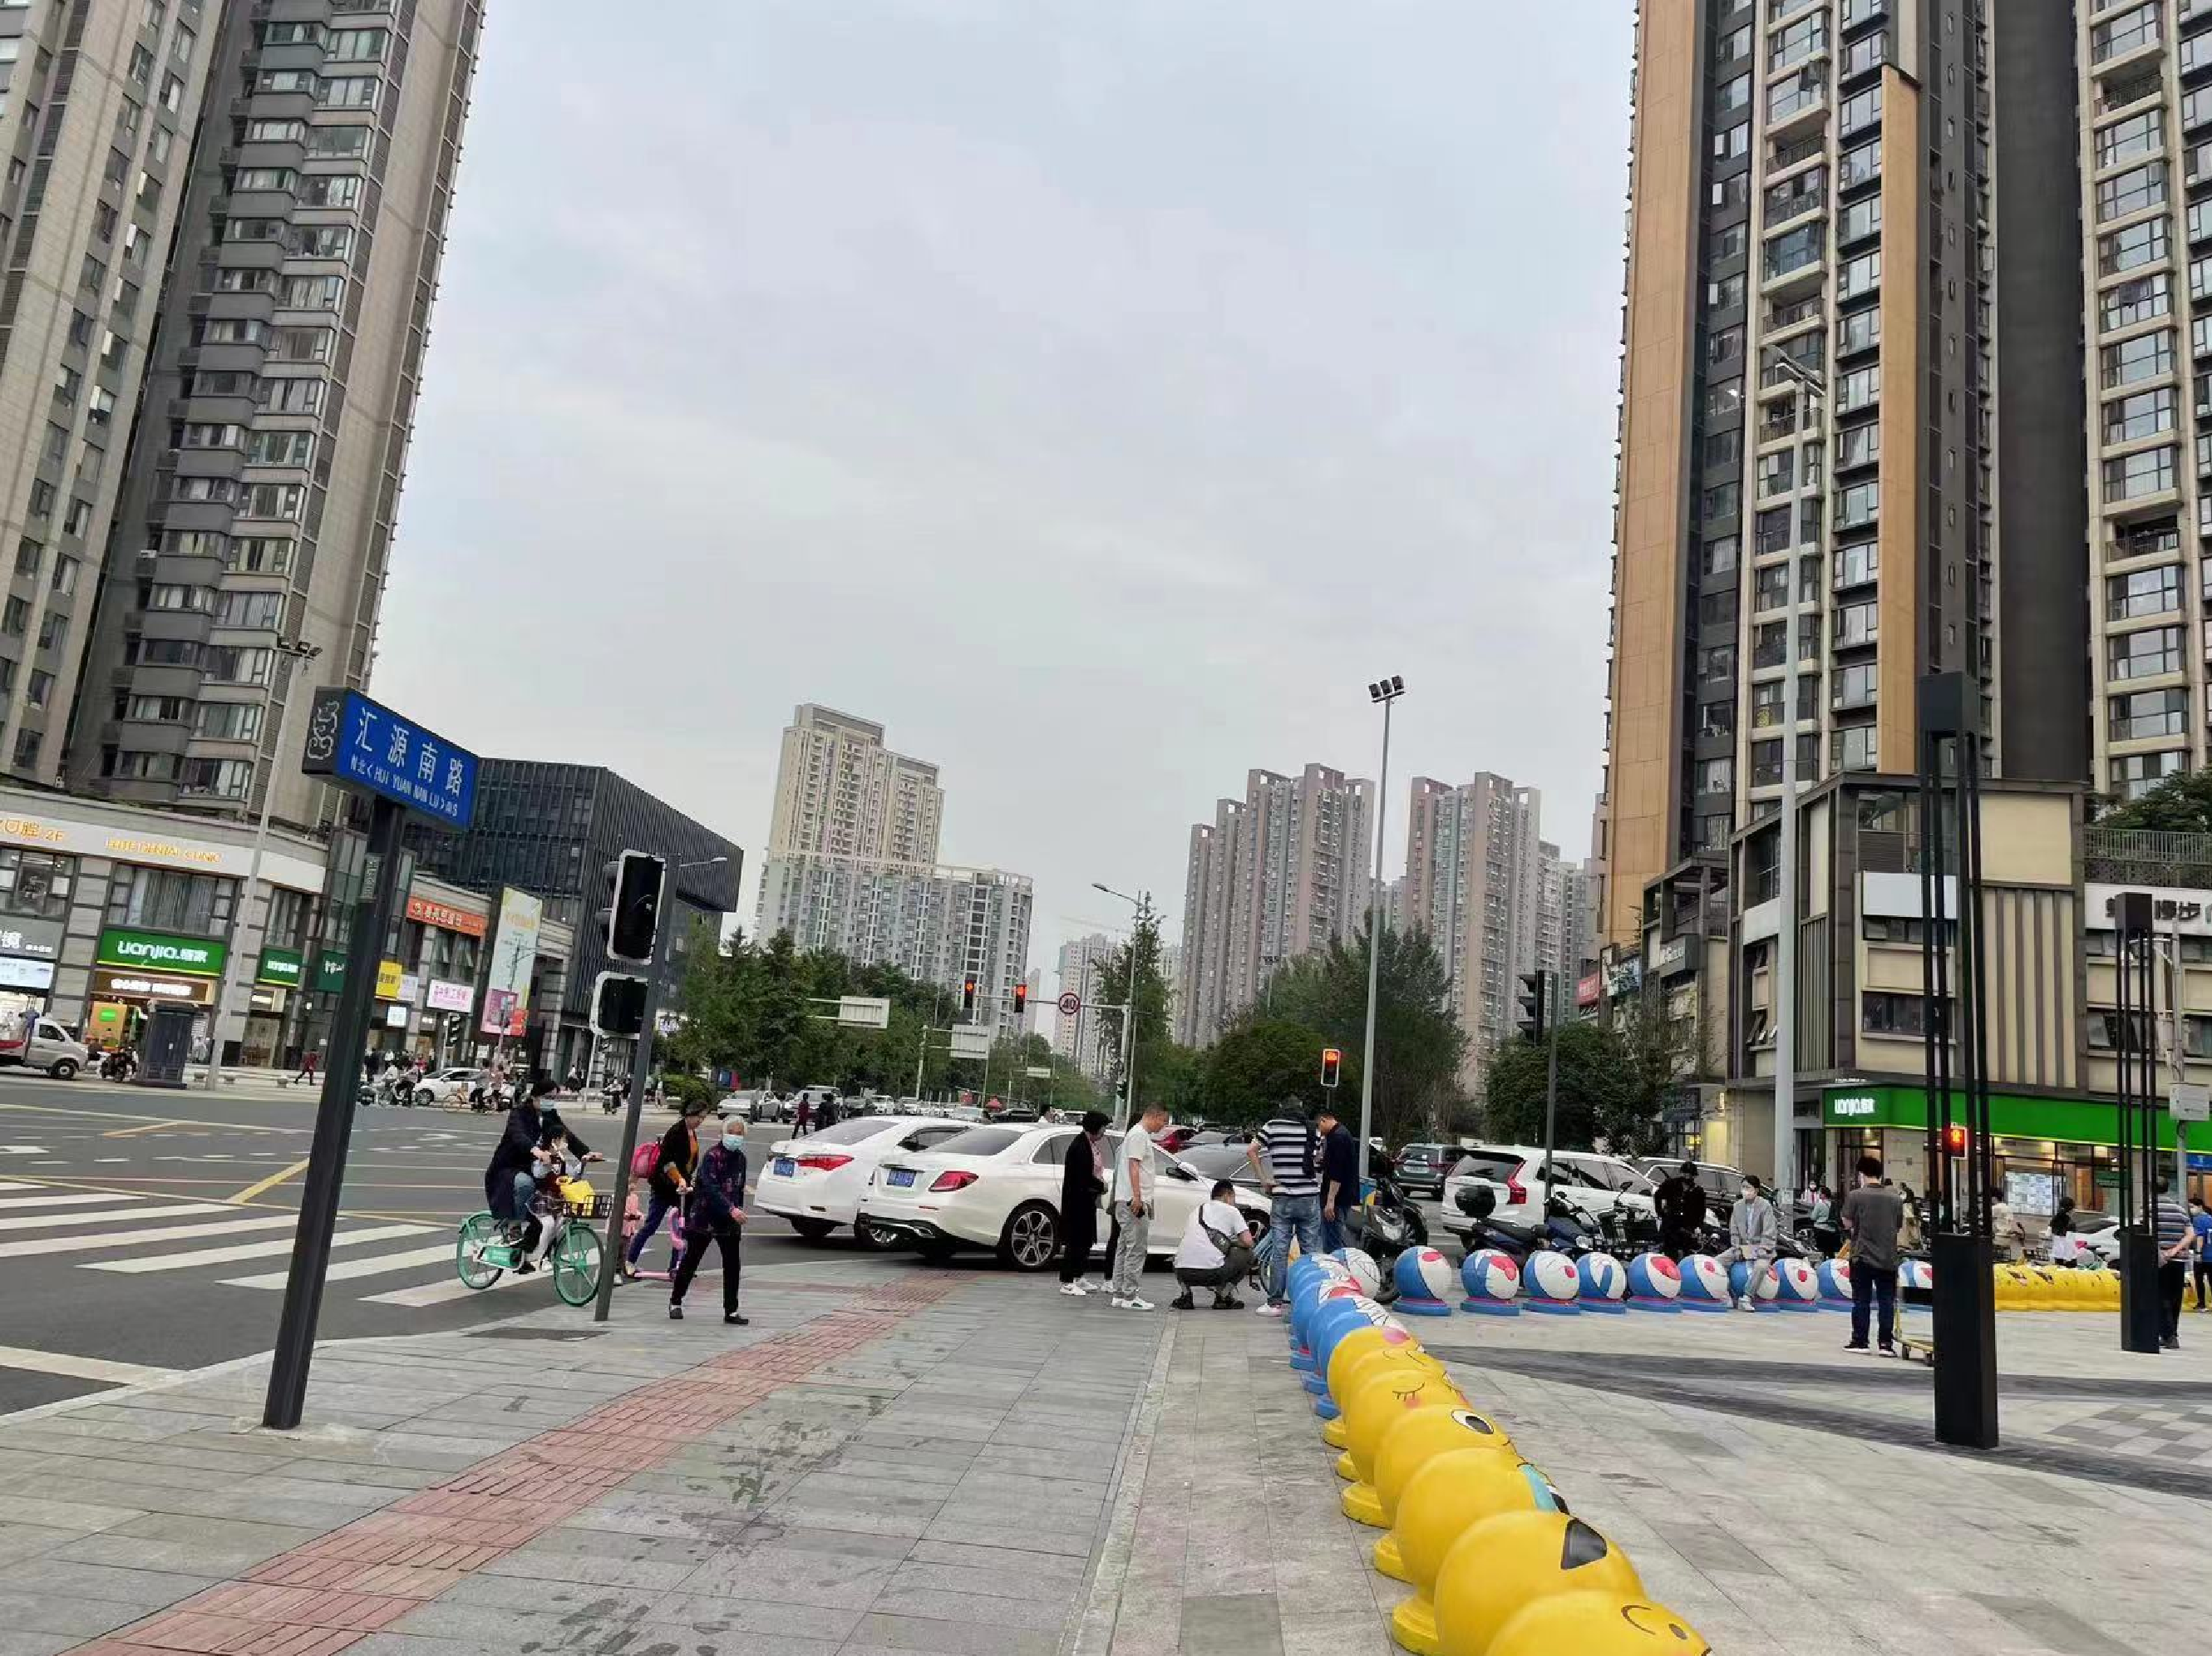
\includegraphics[width=0.9\textwidth]{../figures/typical_sample_lianjia.pdf}
  \caption{Sample of Lianjia's Offline Store with High Clustering}
  \label{fig:typical_sample_lianjia}
  
  This photo was taken in Chengdu, where Lianjia operates over 1,500 offline stores. It is common to see two stores located within a short distance of each other. The green store in the photo is one of Lianjia's offline stores. As you can see, across the street, there are two Lianjia stores, each managed by different store managers. This phenomenon is very common in large Chinese cities and can be found in many markets, see for example Figure \ref{fig:typical_layout_Beijing}.
\end{figure}

\newpage

\begin{figure}[H]
  \centering
  
\includegraphics[width=0.9\textwidth]{../figures/typical_layout_beijing.pdf}
  \caption{Sample of Lianjia's Offline Stores in Beijing}
  \label{fig:typical_layout_Beijing}
  
This figure illustrates the spatial distribution of Lianjia's offline stores in Beijing for the year 2021. The data reveals a significant clustering of stores around major residential buildings, demonstrating a high degree of localization within the real estate brokerage market. This pattern is indicative of the competitive dynamics and agglomeration economies prevalent in the China's real estate sector, where proximity to key infrastructure. The data source is from AutoNavi Map.
\end{figure}

\clearpage

\begin{figure}[h!]
 \centering
    \begin{minipage}{0.328\textwidth}
        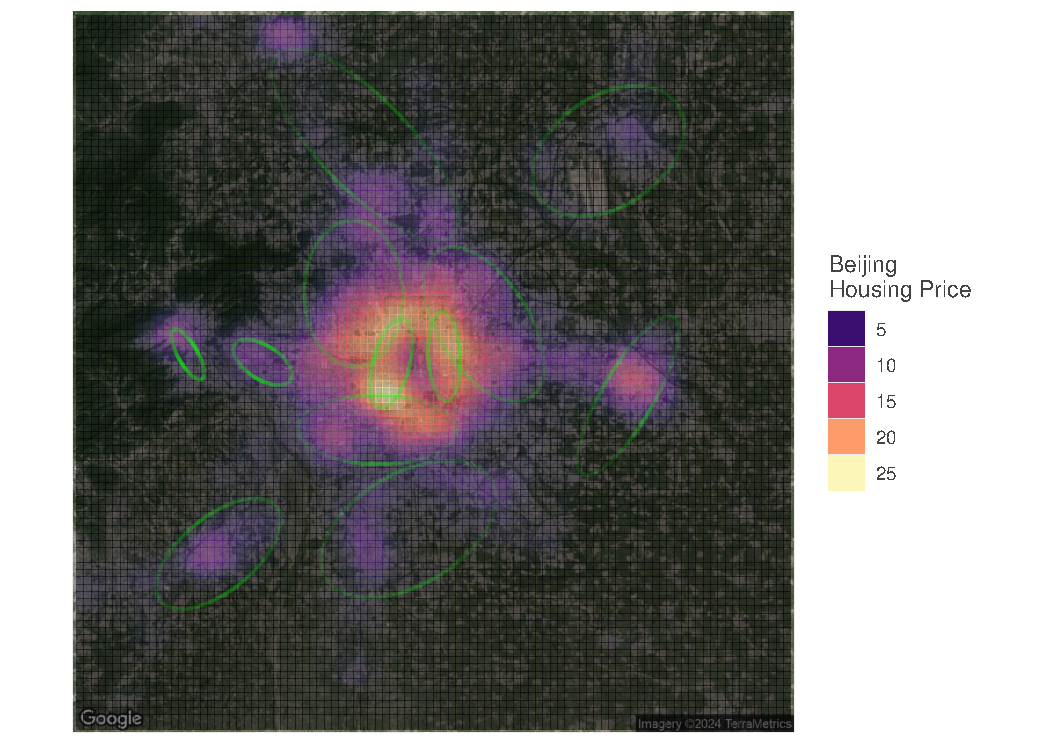
\includegraphics[width=\linewidth]{figures/distribution_of_hp_and_broker/Beijing.pdf}
    \end{minipage}
    \hfill
    \begin{minipage}{0.328\textwidth}
        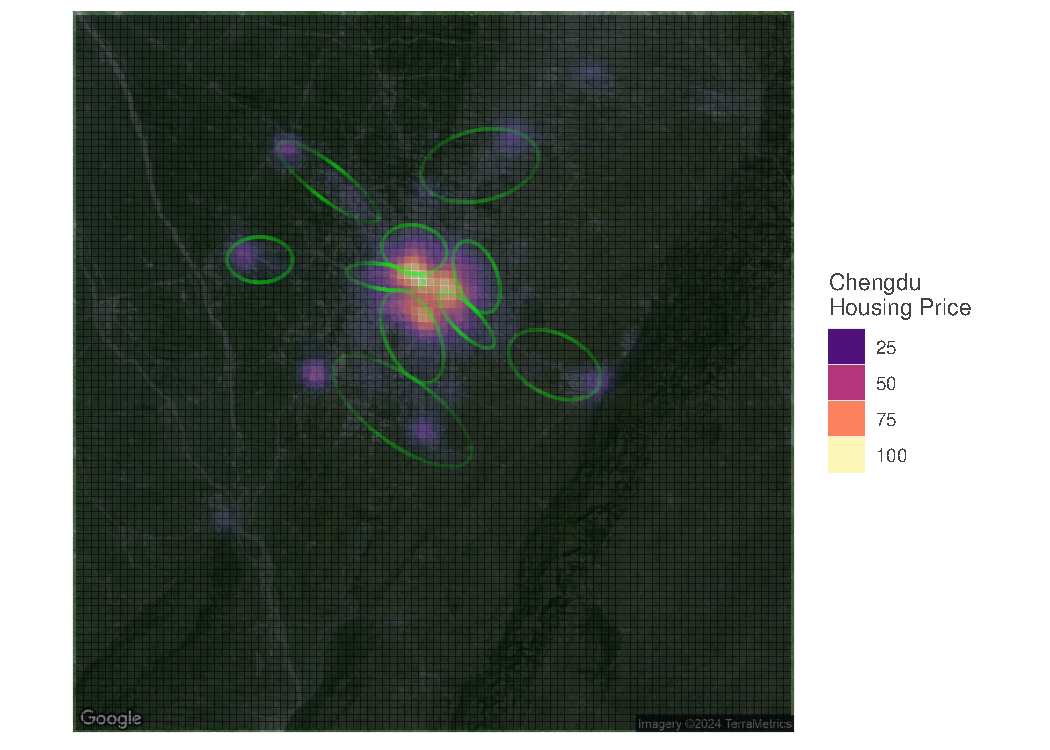
\includegraphics[width=\linewidth]{figures/distribution_of_hp_and_broker/Chengdu.pdf}
    \end{minipage}
    \begin{minipage}{0.328\textwidth}
        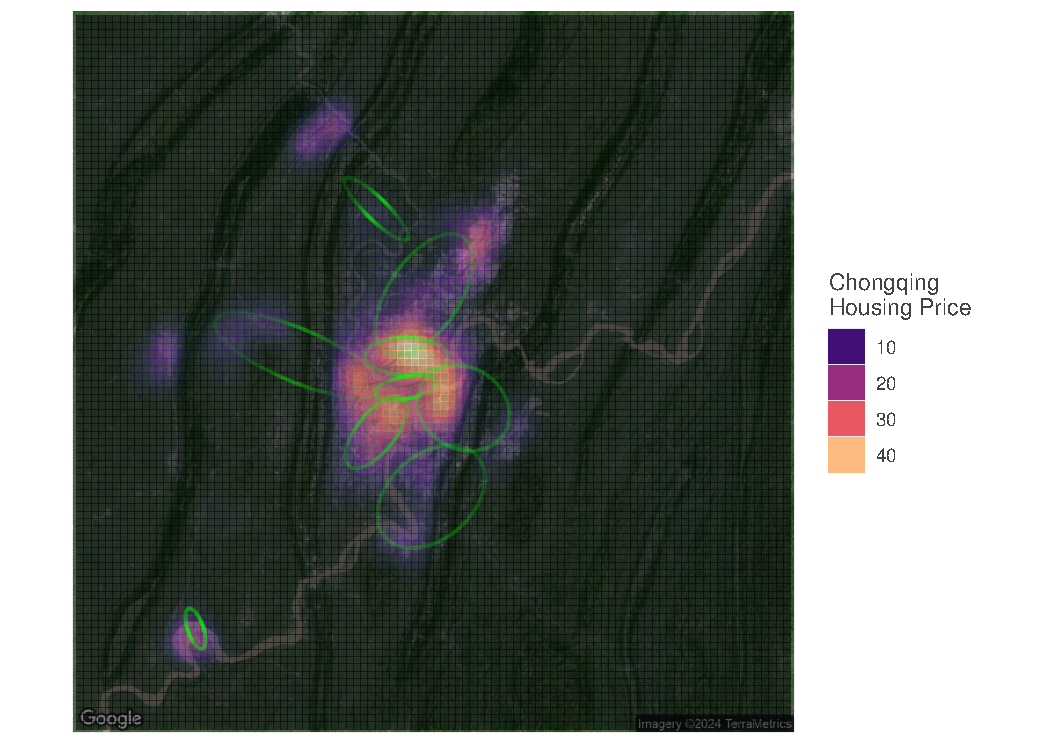
\includegraphics[width=\linewidth]{figures/distribution_of_hp_and_broker/Chongqing.pdf}
    \end{minipage}

    \begin{minipage}{0.328\textwidth}
        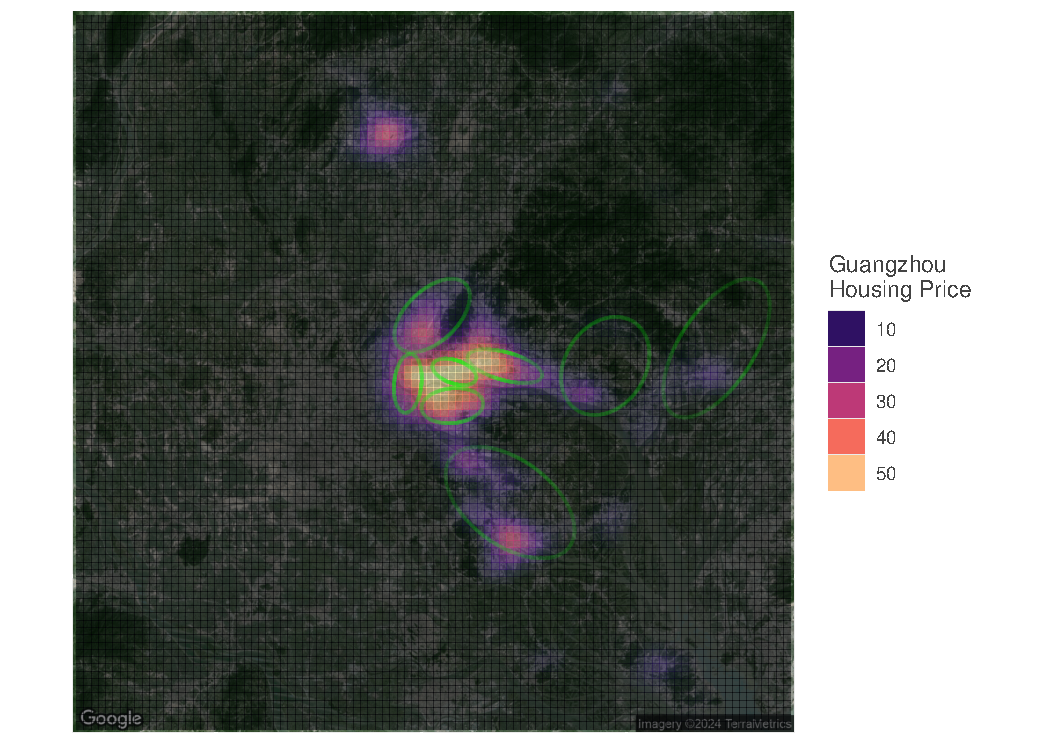
\includegraphics[width=\linewidth]{figures/distribution_of_hp_and_broker/Guangzhou.pdf}
    \end{minipage}
    \hfill
    \begin{minipage}{0.328\textwidth}
        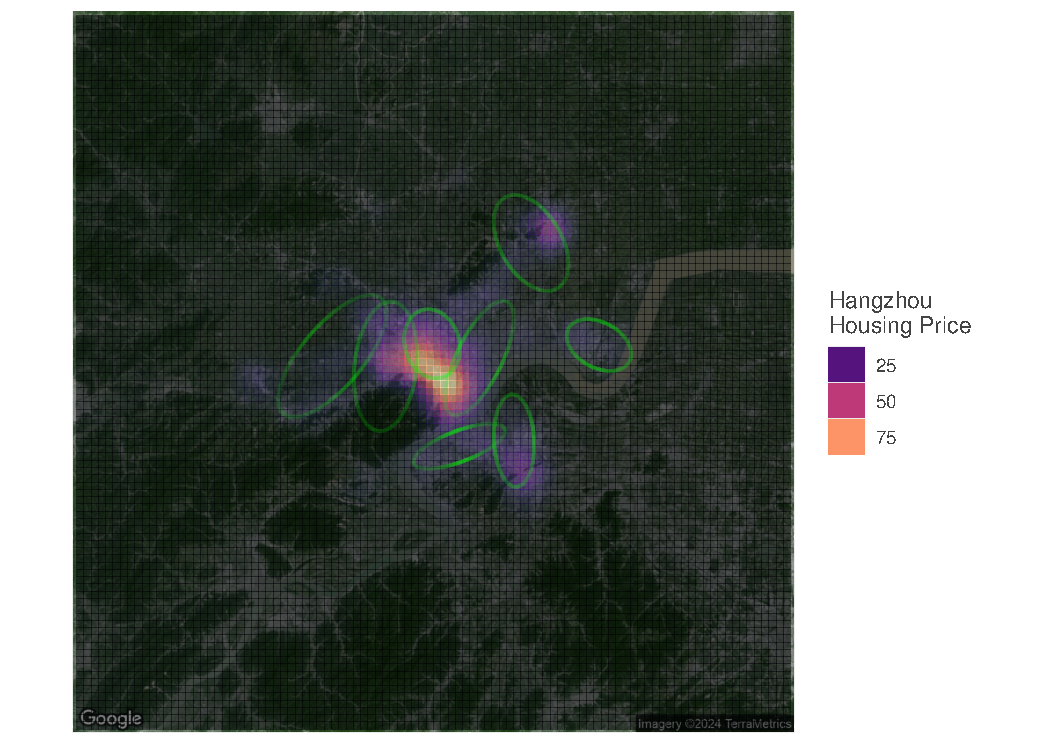
\includegraphics[width=\linewidth]{figures/distribution_of_hp_and_broker/Hangzhou.pdf}
    \end{minipage}
    \begin{minipage}{0.328\textwidth}
        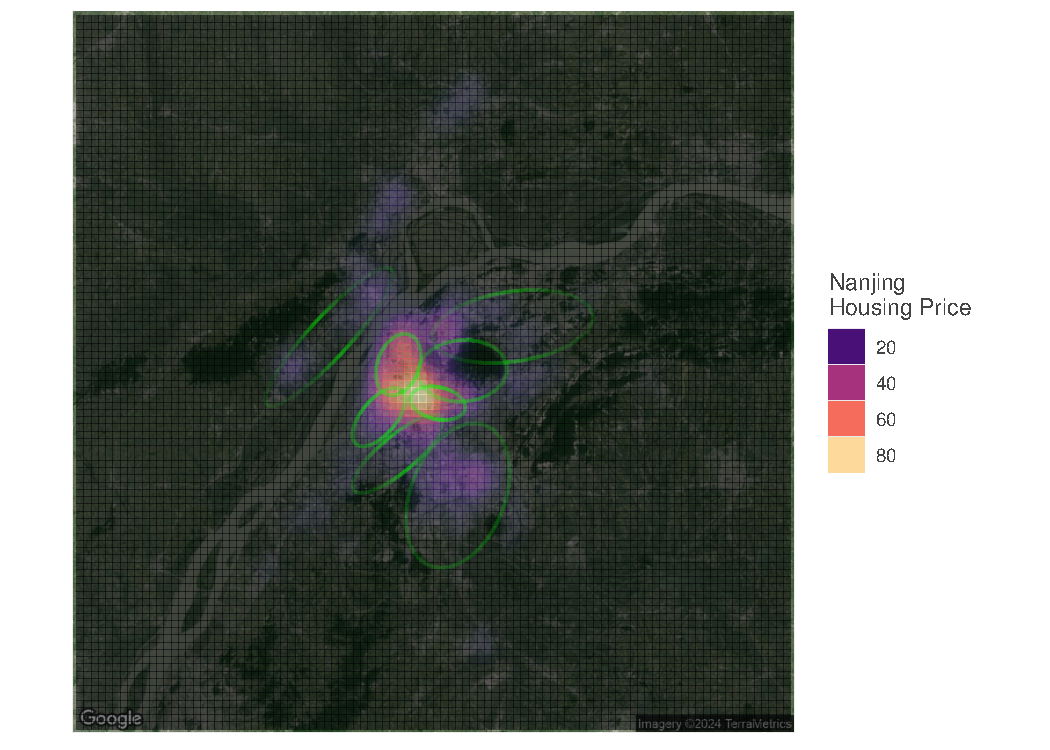
\includegraphics[width=\linewidth]{figures/distribution_of_hp_and_broker/Nanjing.pdf}
    \end{minipage}

    \begin{minipage}{0.328\textwidth}
        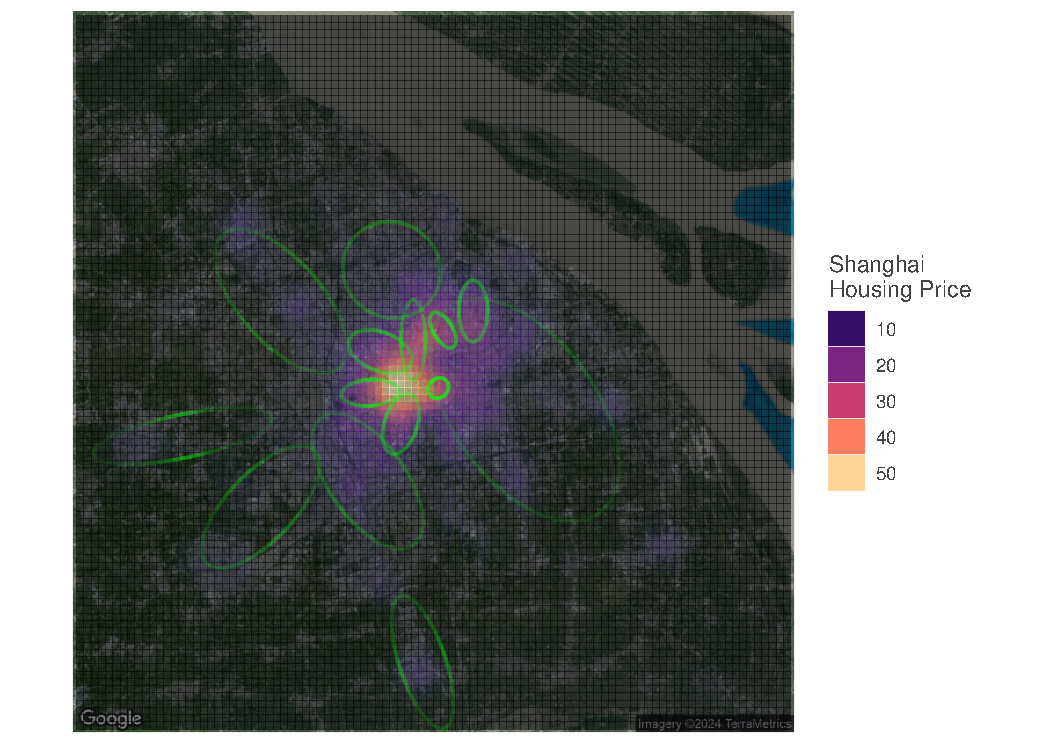
\includegraphics[width=\linewidth]{figures/distribution_of_hp_and_broker/Shanghai.pdf}
    \end{minipage}
    \hfill
    \begin{minipage}{0.328\textwidth}
        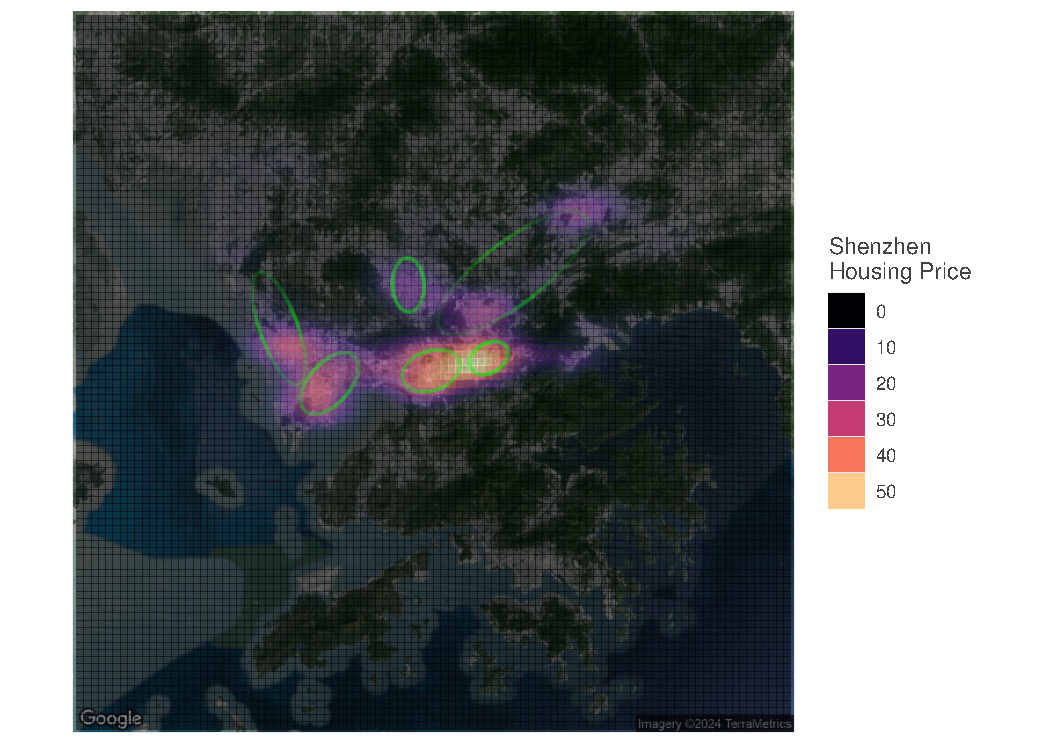
\includegraphics[width=\linewidth]{figures/distribution_of_hp_and_broker/Shenzhen.pdf}
    \end{minipage}
    \begin{minipage}{0.328\textwidth}
        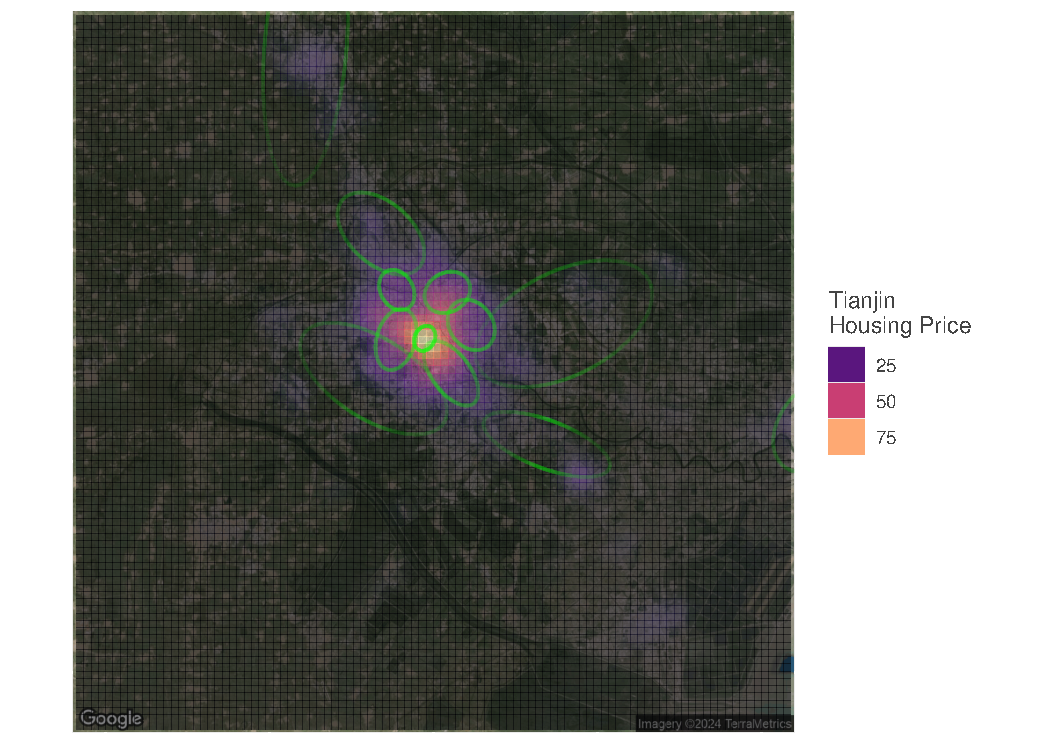
\includegraphics[width=\linewidth]{figures/distribution_of_hp_and_broker/Tianjin.pdf}
    \end{minipage}

    \begin{minipage}{0.328\textwidth}
        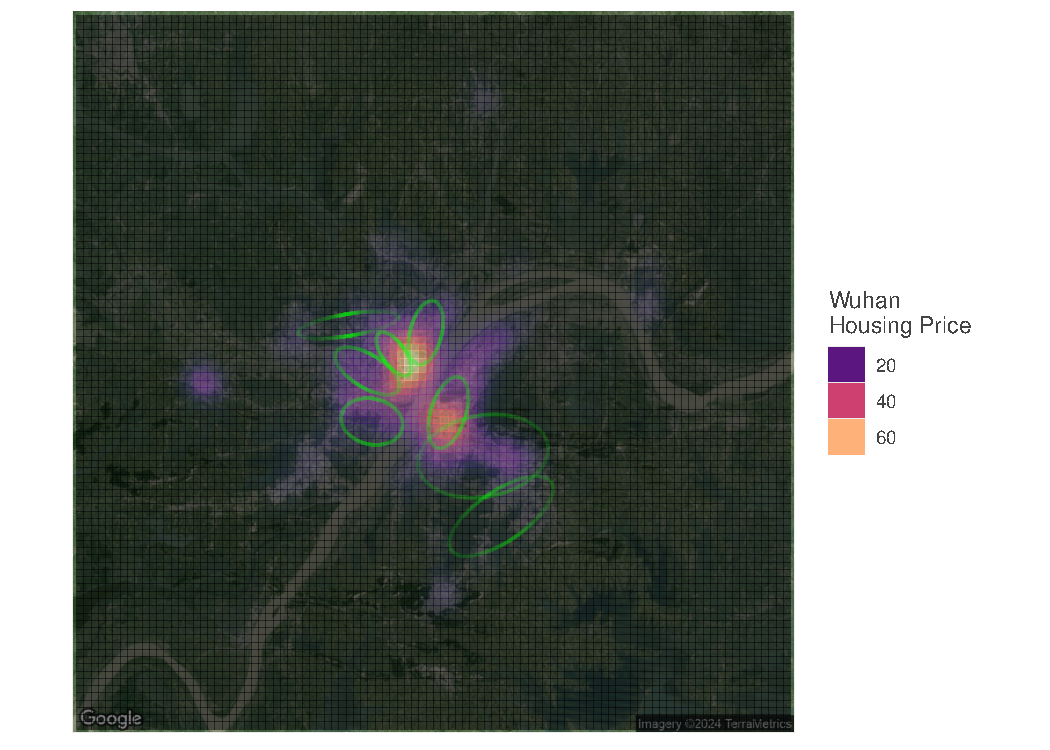
\includegraphics[width=\linewidth]{figures/distribution_of_hp_and_broker/Wuhan.pdf}
    \end{minipage}
    \hfill

\caption{The distribution of housing prices and brokers in different cities}
\label{fig:distribution_of_housing_price_brokers_in_different_cities}

Note: The heat map represents the distribution of housing prices and the standard ellipse represents the distribution of brokers, which is calculated by the mean and standard deviation of the latitude and longitude of brokers. The larger the ellipse, the more sparse the brokerages' distribution is. The Base Map is from Google Map.
 \end{figure}


\clearpage

\begin{figure}[H]
  \centering
  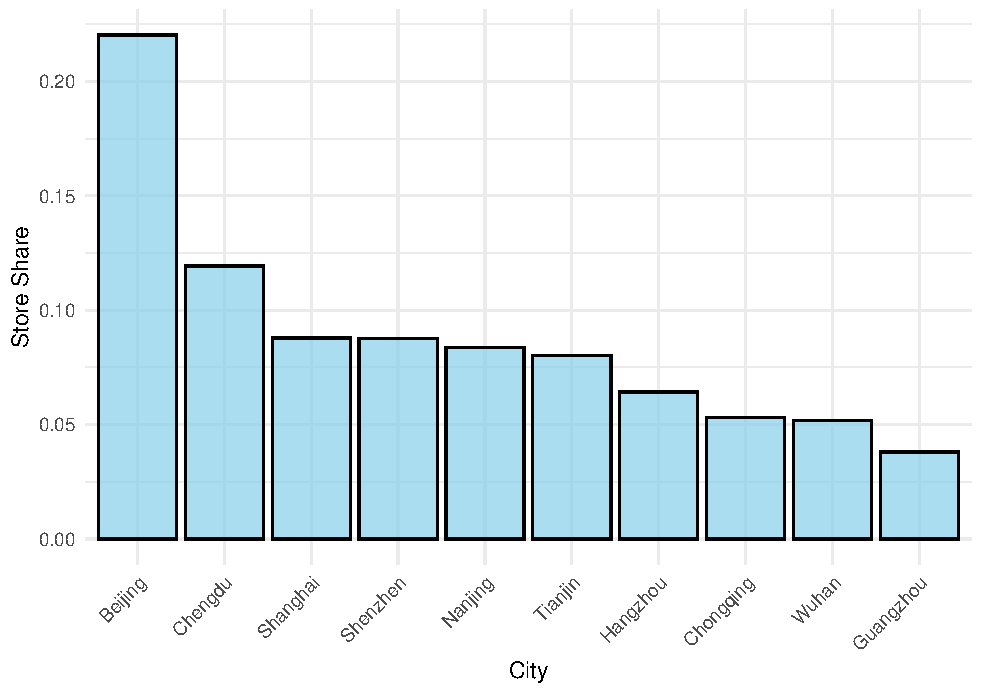
\includegraphics[width=0.9\textwidth]{../figures/distribution_of_ten_cities.pdf}
  \caption{Distribution of Ten Cities's Brokerages Store Shares}
  \label{fig:distribution_store_shares}

  Note: the x-axis is city's name and the y-axis is the offline brokerage's stores share in the city. The data source is from AutoNavi Map.
\end{figure}

\clearpage

\section{Additional RDD Robustness Tests} \label{sec:additional_rdd}
% \input{tab_tex/other-regressions.tex}

Figure \ref{fig:RD_design_Robust} presents the results of the regression discontinuity design (RDD) using the natural logarithm of the dependent variable. The transformation aims to normalize the distribution and stabilize the variance. The findings remain consistent with those obtained using the original dependent variable, indicating the robustness of the treatment effect to changes in the functional form of the dependent variable.

\begin{figure}[ht]
  \centering
  \subfloat[RDD plot with first order polynomial]{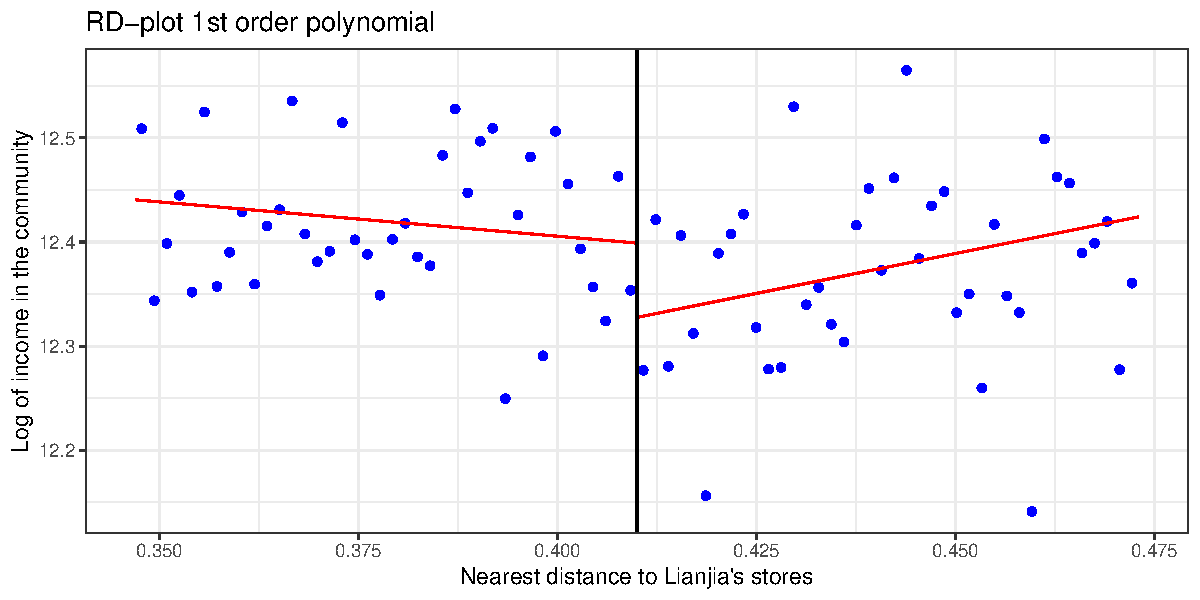
\includegraphics[width=0.5\textwidth]{../figures/RD_Plot_1st_Order_robust.pdf}\label{fig:RD_Plot_1st_Order_Robust}}
  \hfill % Adds horizontal space between figures
  \subfloat[RDD plot with second order polynomial]{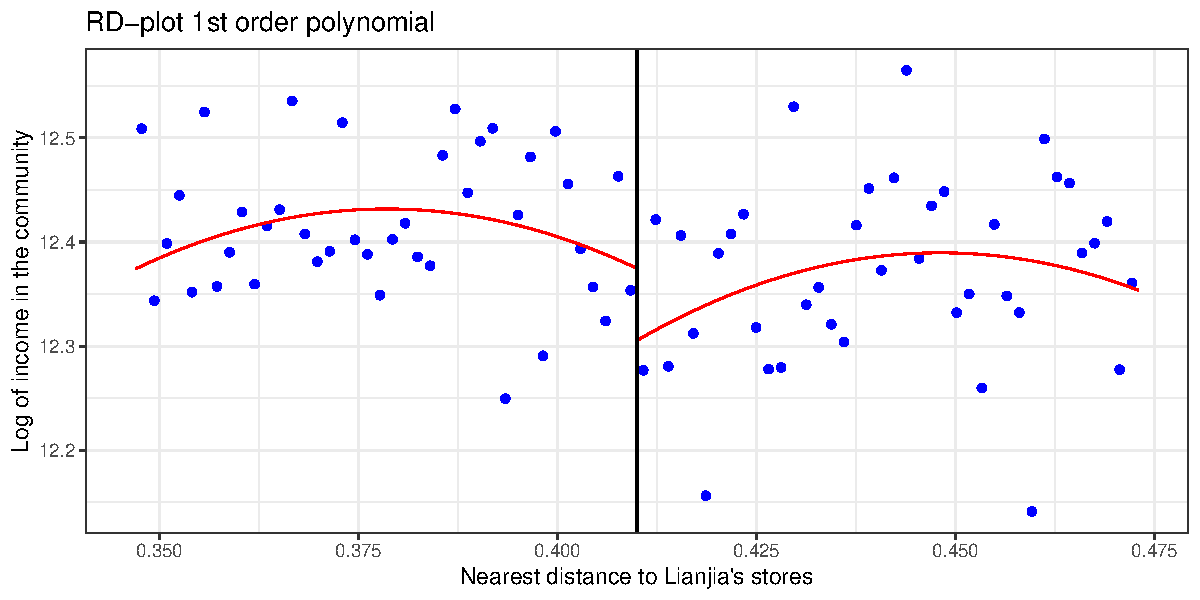
\includegraphics[width=0.5\textwidth]{../figures/RD_Plot_2nd_Order_robust.pdf}\label{fig:RD_Plot_2nd_Order_Robust}}
  \hfill % Adds horizontal space between figures
  \subfloat[RDD plot with third order polynomial]{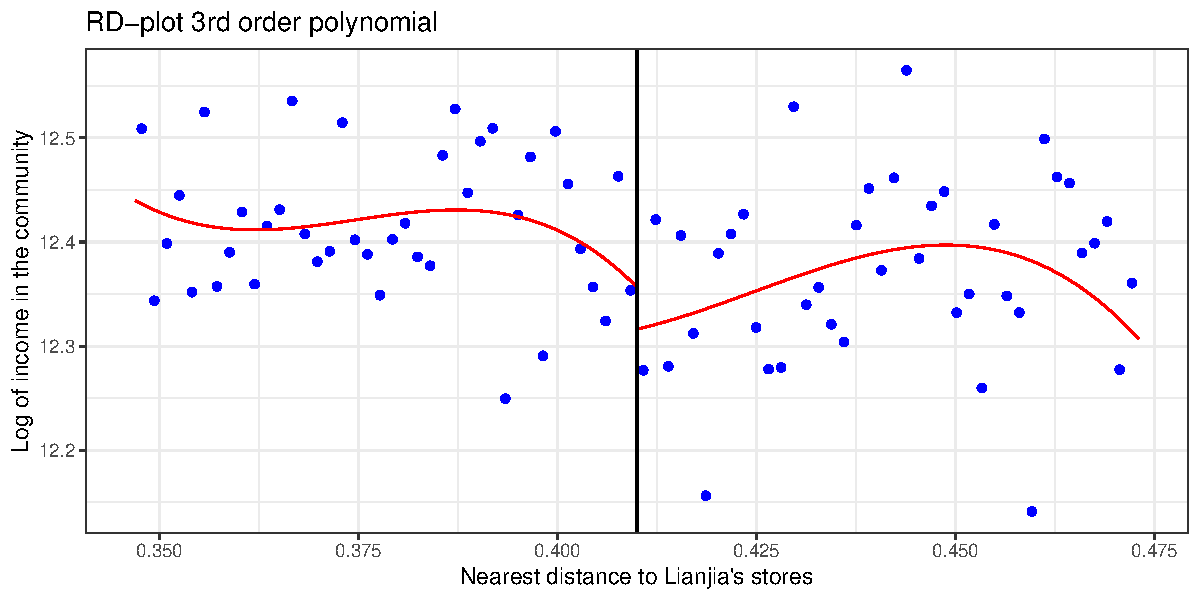
\includegraphics[width=0.5\textwidth]{../figures/RD_Plot_3rd_Order_robust.pdf}\label{fig:RD_Plot_3rd_Order_Robust}}
  \caption{RDD Robustness Check using log(income)}
  \label{fig:RD_design_Robust}
\end{figure}

Table \ref{tab:rd_bandwidth_kernel_results_robust} summarizes the RDD estimates using different bandwidths and kernel functions with the transformed dependent variable. The consistency of the results reaffirms the robustness of the treatment effect and supports the use of a 410-meter radius as the optimal bandwidth for assessing the impact of Lianjia's offline stores.

% latex table generated in R 4.2.0 by xtable 1.8-4 package
% Mon Jul  8 21:13:07 2024
\begin{table}[ht]
\centering
\begin{tabular}{lllllllr}
  \hline
Method & Kernel & Estimate & SE & Z & PValue & Bandwidth & EffectiveObs \\ 
  \hline
mserd & uniform & -0.0584 & 0.0263 & -2.22 & 0.0263 & 0.0773 & 37645 \\ 
  mserd & triangular & -0.0697 & 0.0314 & -2.22 & 0.0267 & 0.066 & 32020 \\ 
  cerrd & uniform & -0.0874 & 0.0361 & -2.42 & 0.0156 & 0.0418 & 19988 \\ 
  cerrd & triangular & -0.0663 & 0.0434 & -1.53 & 0.126 & 0.0357 & 17191 \\ 
   \hline
\end{tabular}
\caption{RD Estimates with Different Bandwidth Selection Methods and Kernels (robust method with log(income))} 
\label{tab:rd_bandwidth_kernel_results_robust}
\end{table}



Table \ref{tab:rd_robust_results} presents the results of the Donut Hole robustness check, where observations within varying distances (5, 7.5, 10, 12.5, 15, 17.5, 20 meters) from the 410-meter cutoff are sequentially excluded. The treatment effect estimates remain robust up to the exclusion of 20\% of the estimated data, demonstrating the stability of the results despite the exclusion of data points near the cutoff.

% latex table generated in R 4.2.0 by xtable 1.8-4 package
% Sun Jun  9 18:04:27 2024
\begin{table}[ht]
\centering
\caption{RD Analysis Donut RD Results with and without Controls} 
\label{tab:rd_robust_results}
\begin{tabular}{llllllll}
  \hline
 &  & \multicolumn{3}{c}{Without Control} & \multicolumn{3}{c}{With Control} \\
Donut Width & Method & Coef & SE & p-value & Coef & SE & p-value \\ 
  \hline
donut\_0.01 & Robust & -0.0527 & 0.0388 & 0.175 & -0.0777 & 0.0522 & 0.136 \\ 
  donut\_0.0125 & Robust & -0.0771 & 0.0434 & 0.076 & -0.11 & 0.0578 & 0.0578 \\ 
  donut\_0.015 & Robust & -0.027 & 0.0485 & 0.578 & -0.113 & 0.0651 & 0.0837 \\ 
  donut\_0.0175 & Robust & -0.0264 & 0.0551 & 0.632 & -0.144 & 0.074 & 0.0517 \\ 
  donut\_0.02 & Robust & 0.0317 & 0.0618 & 0.608 & -0.104 & 0.0836 & 0.214 \\ 
  donut\_0.0225 & Robust & -0.0253 & 0.0708 & 0.721 & -0.115 & 0.0935 & 0.22 \\ 
  donut\_0.025 & Robust & 0.0828 & 0.0806 & 0.304 & 0.0317 & 0.109 & 0.771 \\ 
   \hline
\end{tabular}

Note that the cutoff is 0.41, the main bandwidth is 0.066 and the bias bandwidth is 0.135.
\end{table}



Table \ref{tab:mccrary_results} shows the results of the McCrary density test for manipulation around the cutoff. The p-value is greater than 0.1, indicating no significant discontinuity in the density of the running variable at the cutoff, which supports the assumption of no manipulation.

% latex table generated in R 4.2.0 by xtable 1.8-4 package
% Mon Jul  8 21:17:07 2024
\begin{table}[ht]
\centering
\begin{tabular}{lllllllll}
  \hline
 &  & \multicolumn{3}{c}{Without Control} & \multicolumn{3}{c}{With Control} & \\
Donut Width & Method & Coef & SE & p-value & Coef & SE & p-value & Drop Ratio(\%) \\ 
  \hline
donut\_0.005 & Robust & -47449 & 24227 & 0.0502 & -80978 & 30701 & 0.00835 & 7.85 \\ 
  donut\_0.0075 & Robust & -42335 & 26685 & 0.113 & -79698 & 33726 & 0.0181 & 11.73 \\ 
  donut\_0.01 & Robust & -64934 & 30585 & 0.0337 & -90221 & 38228 & 0.0183 & 15.59 \\ 
  donut\_0.0125 & Robust & -62531 & 34437 & 0.0694 & -78610 & 43377 & 0.07 & 19.48 \\ 
  donut\_0.015 & Robust & -36788 & 39345 & 0.35 & -94673 & 50238 & 0.0595 & 23.66 \\ 
  donut\_0.0175 & Robust & 4018 & 44747 & 0.928 & -76155 & 56672 & 0.179 & 27.88 \\ 
  donut\_0.02 & Robust & 28087 & 49139 & 0.568 & -44578 & 60900 & 0.464 & 31.71 \\ 
   \hline
\end{tabular}
Note that the cutoff is 0.41, the main bandwidth is 0.066 and the bias bandwidth is 0.135.
\caption{RD Analysis Donut RD Results with and without Controls} 
\label{tab:rd_robust_results}
\end{table}




Table \ref{tab:placebo_test_results} presents the results of the placebo tests, where the dependent variable is substituted with other control variables. The absence of significant discontinuity in the placebo tests supports the validity of the observed treatment effect being specifically attributable to the intervention.

% latex table generated in R 4.2.0 by xtable 1.8-4 package
% Sun Jun  9 18:05:45 2024
\begin{table}[ht]
\centering
\caption{Placebo Test Results for Different Covariates} 
\label{tab:placebo_test_results}
\begin{tabular}{llllllr}
  \hline
Covariate & Estimate & SE & Z & PValue & Bandwidth & EffectiveObs \\ 
  \hline
pop & -73.6 & 396 & -0.186 & 0.852 & 0.066 & 32010 \\ 
  light & -0.203 & 0.26 & -0.779 & 0.436 & 0.066 & 32010 \\ 
  price\_concession & -0.000379 & 0.000739 & -0.513 & 0.608 & 0.066 & 31437 \\ 
  ln\_end\_price & -0.0234 & 0.0167 & -1.41 & 0.16 & 0.066 & 32010 \\ 
  ln\_nego\_changes & -0.000518 & 0.0222 & -0.0233 & 0.981 & 0.066 & 32010 \\ 
  ln\_watch\_time & 0.0726 & 0.0682 & 1.06 & 0.288 & 0.066 & 32010 \\ 
  green\_ratio & -0.00161 & 0.00231 & -0.696 & 0.487 & 0.066 & 32010 \\ 
  bedroom & -0.00858 & 0.0176 & -0.487 & 0.626 & 0.066 & 32010 \\ 
  ln\_watch\_people & 0.0542 & 0.0357 & 1.52 & 0.129 & 0.066 & 32010 \\ 
  living\_room & 0.000998 & 0.0113 & 0.0881 & 0.93 & 0.066 & 32010 \\ 
  ln\_negotiation\_period & -0.00648 & 0.0266 & -0.243 & 0.808 & 0.066 & 32010 \\ 
  museum & -0.0544 & 0.0416 & -1.31 & 0.191 & 0.066 & 32010 \\ 
  kind & 0.00667 & 0.136 & 0.0491 & 0.961 & 0.066 & 32010 \\ 
  mid & 0.0124 & 0.0608 & 0.204 & 0.838 & 0.066 & 32010 \\ 
  sub & 0.046 & 0.0244 & 1.89 & 0.059 & 0.066 & 32010 \\ 
  house\_age & 0.209 & 0.275 & 0.76 & 0.447 & 0.066 & 32010 \\ 
  total\_building & -0.275 & 0.829 & -0.332 & 0.74 & 0.066 & 32010 \\ 
   \hline
\end{tabular}
\end{table}



Table \ref{tab:movement_cutoff} shows the results of placebo tests conducted with various cutoff points (325 meters, 350 meters, 400 meters, 420 meters, 450 meters, 500 meters, 650 meters, 700 meters). The findings indicate that the treatment effects are statistically significant and consistent around the 410-meter cutoff, while effects at more distant cutoffs diminish and lose significance. This pattern confirms the localized nature of the intervention's impact.


% latex table generated in R 4.2.0 by xtable 1.8-4 package
% Mon Jul  8 21:20:28 2024
\begin{table}[ht]
\centering
\caption{Placebo Test Results for Different Cutoff Point} 
\label{tab:movement_cutoff}
\begin{tabular}{rlllllr}
  \hline
Cutoff & Estimate & SE & Z & PValue & Bandwidth & EffectiveObs \\ 
  \hline
0.32 & -33154 & 16261 & -2.04 & 0.0415 & 0.0965 & 58710 \\ 
  0.35 & 2112 & 13951 & 0.151 & 0.88 & 0.132 & 75514 \\ 
  0.40 & -25930 & 19778 & -1.31 & 0.19 & 0.0764 & 38332 \\ 
  0.42 & -12532 & 18043 & -0.695 & 0.487 & 0.0855 & 40529 \\ 
  0.45 & -22806 & 17952 & -1.27 & 0.204 & 0.0858 & 36968 \\ 
  0.50 & 25778 & 15534 & 1.66 & 0.097 & 0.133 & 49373 \\ 
  0.65 & 47140 & 21425 & 2.2 & 0.0278 & 0.092 & 20096 \\ 
  0.70 & -32584 & 19286 & -1.69 & 0.0911 & 0.121 & 22549 \\ 
   \hline
\end{tabular}
\end{table}



% Imbens, G. W., & Lemieux, T. (2008). Regression Discontinuity Designs: A Guide to Practice. Journal of Econometrics, 142(2), 615-635.
% Lee, D. S., & Lemieux, T. (2010). Regression Discontinuity Designs in Economics. Journal of Economic Literature, 48(2), 281-355.

\newpage

\section{Additional Robustness Check of Main Results} \label{sec:additional_robustness}

\subsection{Additional Robustness Check for the Offline Expansion Effect} \label{subsec:expansion_effect}

In this section, we report the robustness check of DID model. Table \ref{tab:robustness_check_additional_1}, Table \ref{tab:robustness_check_additional_2} display the estimation outcomes without the inclusion of additional control variables. By comparing these results with those obtained when controls are included, we observe that the estimates remain consistent across different model specifications. This consistency indicates the robustness of our findings, reinforcing the validity of our conclusions.

\begin{table}[H]
  \begin{center}
    \begin{scriptsize}
      \caption{Robustness Check of Lianjia's Offline Expansion Effect}
      \label{tab:robustness_check_additional_1}
      {
\def\sym#1{\ifmmode^{#1}\else\(^{#1}\)\fi}
\begin{adjustbox}{max width=\textwidth}
\begin{tabular}{l*{8}{c}}
\toprule
            &\multicolumn{1}{c}{(1)}&\multicolumn{1}{c}{(2)}&\multicolumn{1}{c}{(3)}&\multicolumn{1}{c}{(4)}&\multicolumn{1}{c}{(5)}&\multicolumn{1}{c}{(6)}&\multicolumn{1}{c}{(7)}&\multicolumn{1}{c}{(8)}\\
            &\multicolumn{1}{c}{log(number)}&\multicolumn{1}{c}{log(number)}&\multicolumn{1}{c}{log(number)}&\multicolumn{1}{c}{log(number)}&\multicolumn{1}{c}{log(lead times)}&\multicolumn{1}{c}{log(lead times)}&\multicolumn{1}{c}{log(lead times)}&\multicolumn{1}{c}{log(lead times)}\\
\midrule
pre2        &      -0.010         &      -0.009         &      -0.008         &      -0.008         &      -0.017         &      -0.019\sym{*}  &      -0.019\sym{*}  &      -0.019\sym{*}  \\
            &     (0.015)         &     (0.014)         &     (0.014)         &     (0.014)         &     (0.015)         &     (0.011)         &     (0.011)         &     (0.011)         \\
\addlinespace
entry       &       0.102\sym{***}&       0.091\sym{***}&       0.091\sym{***}&       0.091\sym{***}&       0.031\sym{***}&       0.022\sym{***}&       0.023\sym{***}&       0.023\sym{***}\\
            &     (0.012)         &     (0.012)         &     (0.012)         &     (0.012)         &     (0.012)         &     (0.008)         &     (0.008)         &     (0.008)         \\
\addlinespace
post1       &       0.060\sym{***}&       0.049\sym{***}&       0.048\sym{***}&       0.048\sym{***}&       0.038\sym{***}&       0.031\sym{***}&       0.031\sym{***}&       0.031\sym{***}\\
            &     (0.013)         &     (0.012)         &     (0.012)         &     (0.012)         &     (0.012)         &     (0.009)         &     (0.009)         &     (0.009)         \\
\addlinespace
post2       &       0.019         &       0.007         &       0.007         &       0.007         &       0.022\sym{*}  &       0.011         &       0.011         &       0.011         \\
            &     (0.013)         &     (0.013)         &     (0.013)         &     (0.013)         &     (0.013)         &     (0.010)         &     (0.010)         &     (0.010)         \\
\addlinespace
post3       &       0.018         &       0.011         &       0.010         &       0.010         &       0.022         &       0.020\sym{*}  &       0.020\sym{*}  &       0.020\sym{*}  \\
            &     (0.015)         &     (0.015)         &     (0.015)         &     (0.015)         &     (0.013)         &     (0.011)         &     (0.011)         &     (0.011)         \\
\addlinespace
Brokerage Control &                     &  \checkmark         &  \checkmark         &  \checkmark         &                     &  \checkmark         &  \checkmark         &  \checkmark         \\
\addlinespace
Hedonic Control &                     &                     &  \checkmark         &  \checkmark         &                     &                     &  \checkmark         &  \checkmark         \\
\addlinespace
Transaction Control &                     &                     &                     &  \checkmark         &                     &                     &                     &  \checkmark         \\
Regional Control & & & & & & & & \\
\midrule
\(N\)       &      103966         &      103966         &      103966         &      103966         &      103966         &      103966         &      103966         &      103966         \\
R-squared   &       0.806         &       0.814         &       0.814         &       0.815         &       0.837         &       0.911         &       0.911         &       0.912         \\
\bottomrule
\multicolumn{9}{l}{\footnotesize Standard errors in parentheses}\\
\multicolumn{9}{l}{\footnotesize \sym{*} \(p<0.1\), \sym{**} \(p<0.05\), \sym{***} \(p<0.01\)}\\
\end{tabular}
\end{adjustbox}
}

    
    Note: we omit all the control variables in the regression model, and detailed descriptions can be seen from Table \ref{tab:statistical_district} and Table \ref{tab:statistical_individual}.
    \end{scriptsize}
  \end{center}
\end{table}

\begin{table}[H]
  \begin{center}
    \begin{scriptsize}
      \caption{Robustness Check of Lianjia's Offline Expansion Effect (Continued)}
      \label{tab:robustness_check_additional_2}
      {
\def\sym#1{\ifmmode^{#1}\else\(^{#1}\)\fi}
\begin{adjustbox}{max width=\textwidth}
\begin{tabular}{l*{8}{c}}
\toprule
            &\multicolumn{1}{c}{(1)}&\multicolumn{1}{c}{(2)}&\multicolumn{1}{c}{(3)}&\multicolumn{1}{c}{(4)}&\multicolumn{1}{c}{(5)}&\multicolumn{1}{c}{(6)}&\multicolumn{1}{c}{(7)}&\multicolumn{1}{c}{(8)}\\
            &\multicolumn{1}{c}{log(negotiation period)}&\multicolumn{1}{c}{log(negotiation period)}&\multicolumn{1}{c}{log(negotiation period)}&\multicolumn{1}{c}{log(negotiation period)}&\multicolumn{1}{c}{price concession}&\multicolumn{1}{c}{price concession}&\multicolumn{1}{c}{price concession}&\multicolumn{1}{c}{price concession}\\
\midrule
pre2        &      -0.018         &      -0.016         &      -0.016         &      -0.014         &      -0.027         &      -0.027         &      -0.033         &      -0.033         \\
            &     (0.013)         &     (0.014)         &     (0.014)         &     (0.014)         &     (0.028)         &     (0.026)         &     (0.026)         &     (0.026)         \\
\addlinespace
entry       &      -0.018\sym{*}  &      -0.009         &      -0.009         &      -0.007         &       0.054\sym{***}&       0.051\sym{**} &       0.048\sym{**} &       0.044\sym{**} \\
            &     (0.010)         &     (0.010)         &     (0.010)         &     (0.010)         &     (0.019)         &     (0.020)         &     (0.020)         &     (0.020)         \\
\addlinespace
post1       &      -0.016         &      -0.012         &      -0.012         &      -0.012         &       0.053\sym{**} &       0.048\sym{**} &       0.046\sym{**} &       0.045\sym{*}  \\
            &     (0.012)         &     (0.010)         &     (0.010)         &     (0.010)         &     (0.023)         &     (0.023)         &     (0.024)         &     (0.023)         \\
\addlinespace
post2       &       0.002         &       0.006         &       0.005         &       0.007         &       0.020         &       0.013         &       0.010         &       0.006         \\
            &     (0.012)         &     (0.011)         &     (0.011)         &     (0.011)         &     (0.024)         &     (0.024)         &     (0.025)         &     (0.024)         \\
\addlinespace
post3       &      -0.021         &      -0.008         &      -0.008         &      -0.007         &       0.018         &       0.008         &       0.005         &       0.002         \\
            &     (0.016)         &     (0.015)         &     (0.015)         &     (0.015)         &     (0.027)         &     (0.027)         &     (0.027)         &     (0.027)         \\
\addlinespace
Brokerage Control &                     &  \checkmark         &  \checkmark         &  \checkmark         &                     &  \checkmark         &  \checkmark         &  \checkmark         \\
\addlinespace
Hedonic Control &                     &                     &  \checkmark         &  \checkmark         &                     &                     &  \checkmark         &  \checkmark         \\
\addlinespace
Transaction Control &                     &                     &                     &  \checkmark         &                     &                     &                     &  \checkmark         \\
Regional Control & & & & & & & & \\
\midrule
\(N\)       &      867874         &      867874         &      867874         &      867874         &      845953         &      845953         &      845953         &      845953         \\
R-squared   &       0.227         &       0.499         &       0.499         &       0.504         &       0.213         &       0.223         &       0.223         &       0.227         \\
\bottomrule
\multicolumn{9}{l}{\footnotesize Standard errors in parentheses}\\
\multicolumn{9}{l}{\footnotesize \sym{*} \(p<0.1\), \sym{**} \(p<0.05\), \sym{***} \(p<0.01\)}\\
\end{tabular}
\end{adjustbox}
}

    
    Note: we omit all the control variables in the regression model, and detailed descriptions can be seen from Table \ref{tab:statistical_district} and Table \ref{tab:statistical_individual}.
    \end{scriptsize}
  \end{center}
\end{table}

Table \ref{tab:robustness_check_platform_1} and \ref{tab:robustness_check_platform_2} shows the results or our estimation with or without additional control variables, and the results are consistent.

\begin{table}[H]
  \begin{center}
    \begin{scriptsize}
      \caption{Robustness Check of Lianjia's Platform-Mediated Consolidation Effect}
      \label{tab:robustness_check_platform_1}
      {
\def\sym#1{\ifmmode^{#1}\else\(^{#1}\)\fi}
\begin{adjustbox}{max width=\textwidth}
\begin{tabular}{l*{8}{c}}
\toprule
            &\multicolumn{1}{c}{(1)}&\multicolumn{1}{c}{(2)}&\multicolumn{1}{c}{(3)}&\multicolumn{1}{c}{(4)}&\multicolumn{1}{c}{(5)}&\multicolumn{1}{c}{(6)}&\multicolumn{1}{c}{(7)}&\multicolumn{1}{c}{(8)}\\
            &\multicolumn{1}{c}{log(number)}&\multicolumn{1}{c}{log(number)}&\multicolumn{1}{c}{log(number)}&\multicolumn{1}{c}{log(number)}&\multicolumn{1}{c}{log(lead times)}&\multicolumn{1}{c}{log(lead times)}&\multicolumn{1}{c}{log(lead times)}&\multicolumn{1}{c}{log(lead times)}\\
\midrule
pre1\_treatment&      -0.008         &      -0.006         &      -0.007         &      -0.006         &       0.011         &       0.006         &       0.005         &       0.005         \\
            &     (0.010)         &     (0.010)         &     (0.010)         &     (0.010)         &     (0.010)         &     (0.008)         &     (0.008)         &     (0.008)         \\
\addlinespace
treatment   &      -0.002         &       0.000         &      -0.000         &       0.000         &      -0.005         &      -0.005         &      -0.005         &      -0.005         \\
            &     (0.010)         &     (0.010)         &     (0.010)         &     (0.010)         &     (0.011)         &     (0.008)         &     (0.008)         &     (0.008)         \\
\addlinespace
post1\_treatment&       0.063\sym{***}&       0.061\sym{***}&       0.061\sym{***}&       0.061\sym{***}&       0.046\sym{***}&       0.031\sym{***}&       0.031\sym{***}&       0.031\sym{***}\\
            &     (0.011)         &     (0.011)         &     (0.011)         &     (0.011)         &     (0.011)         &     (0.009)         &     (0.009)         &     (0.009)         \\
\addlinespace
post2\_treatment&       0.065\sym{***}&       0.062\sym{***}&       0.062\sym{***}&       0.062\sym{***}&       0.047\sym{***}&       0.029\sym{***}&       0.029\sym{***}&       0.029\sym{***}\\
            &     (0.012)         &     (0.012)         &     (0.012)         &     (0.012)         &     (0.012)         &     (0.010)         &     (0.010)         &     (0.010)         \\
\addlinespace
post3\_treatment&       0.032\sym{**} &       0.030\sym{*}  &       0.029\sym{*}  &       0.029\sym{*}  &       0.024         &       0.013         &       0.012         &       0.013         \\
            &     (0.015)         &     (0.015)         &     (0.015)         &     (0.015)         &     (0.017)         &     (0.013)         &     (0.013)         &     (0.013)         \\
\addlinespace
Brokerage Control &                     &  \checkmark         &  \checkmark         &  \checkmark         &                     &  \checkmark         &  \checkmark         &  \checkmark         \\
\addlinespace
Hedonic Control &                     &                     &  \checkmark         &  \checkmark         &                     &                     &  \checkmark         &  \checkmark         \\
\addlinespace
Transaction Control &                     &                     &                     &  \checkmark         &                     &                     &                     &  \checkmark         \\
Regional Control & & & & & & & & \\
\midrule
\(N\)       &      133420         &      133420         &      133420         &      133420         &      133420         &      133420         &      133420         &      133420         \\
R-squared   &       0.847         &       0.852         &       0.852         &       0.852         &       0.865         &       0.924         &       0.924         &       0.924         \\
\bottomrule
\multicolumn{9}{l}{\footnotesize Standard errors in parentheses}\\
\multicolumn{9}{l}{\footnotesize \sym{*} \(p<0.1\), \sym{**} \(p<0.05\), \sym{***} \(p<0.01\)}\\
\end{tabular}
\end{adjustbox}
}

    
    Note: we omit all the control variables in the regression model, and detailed descriptions can be seen from Table \ref{tab:statistical_district} and Table \ref{tab:statistical_individual}.
    \end{scriptsize}
  \end{center}
\end{table}

\begin{table}
  \begin{center}
    \begin{scriptsize}
      \caption{Robustness Check of Lianjia's Platform-Mediated Consolidation Effect (Continued)}
      \label{tab:robustness_check_platform_2}
      {
\def\sym#1{\ifmmode^{#1}\else\(^{#1}\)\fi}
\begin{adjustbox}{max width=\textwidth}
\begin{tabular}{l*{8}{c}}
\toprule
            &\multicolumn{1}{c}{(1)}&\multicolumn{1}{c}{(2)}&\multicolumn{1}{c}{(3)}&\multicolumn{1}{c}{(4)}&\multicolumn{1}{c}{(5)}&\multicolumn{1}{c}{(6)}&\multicolumn{1}{c}{(7)}&\multicolumn{1}{c}{(8)}\\
            &\multicolumn{1}{c}{log(negotiation period)}&\multicolumn{1}{c}{log(negotiation period)}&\multicolumn{1}{c}{log(negotiation period)}&\multicolumn{1}{c}{log(negotiation period)}&\multicolumn{1}{c}{price concession}&\multicolumn{1}{c}{price concession}&\multicolumn{1}{c}{price concession}&\multicolumn{1}{c}{price concession}\\
\midrule
pre1\_treatment&      -0.017\sym{*}  &      -0.015         &      -0.016         &      -0.014         &       0.007         &       0.007         &       0.005         &       0.003         \\
            &     (0.010)         &     (0.010)         &     (0.010)         &     (0.009)         &     (0.021)         &     (0.021)         &     (0.021)         &     (0.021)         \\
\addlinespace
treatment   &      -0.003         &      -0.005         &      -0.006         &      -0.005         &      -0.000         &       0.002         &       0.004         &       0.001         \\
            &     (0.011)         &     (0.011)         &     (0.011)         &     (0.011)         &     (0.022)         &     (0.021)         &     (0.021)         &     (0.021)         \\
\addlinespace
post1\_treatment&       0.002         &      -0.003         &      -0.004         &      -0.004         &       0.042\sym{*}  &       0.044\sym{*}  &       0.047\sym{*}  &       0.045\sym{*}  \\
            &     (0.013)         &     (0.013)         &     (0.013)         &     (0.013)         &     (0.025)         &     (0.024)         &     (0.024)         &     (0.024)         \\
\addlinespace
post2\_treatment&       0.001         &      -0.005         &      -0.007         &      -0.007         &       0.074\sym{**} &       0.074\sym{**} &       0.080\sym{***}&       0.077\sym{***}\\
            &     (0.016)         &     (0.015)         &     (0.015)         &     (0.016)         &     (0.030)         &     (0.029)         &     (0.030)         &     (0.030)         \\
\addlinespace
post3\_treatment&      -0.012         &      -0.006         &      -0.008         &      -0.008         &       0.047         &       0.048         &       0.051         &       0.050         \\
            &     (0.019)         &     (0.018)         &     (0.018)         &     (0.019)         &     (0.040)         &     (0.041)         &     (0.041)         &     (0.041)         \\
\addlinespace
Brokerage Control &                     &  \checkmark         &  \checkmark         &  \checkmark         &                     &  \checkmark         &  \checkmark         &  \checkmark         \\
\addlinespace
Hedonic Control &                     &                     &  \checkmark         &  \checkmark         &                     &                     &  \checkmark         &  \checkmark         \\
\addlinespace
Transaction Control &                     &                     &                     &  \checkmark         &                     &                     &                     &  \checkmark         \\
Regional Control & & & & & & & & \\
\midrule
\(N\)       &     1268778         &     1268778         &     1268778         &     1268778         &     1246875         &     1246875         &     1246875         &     1246875         \\
R-squared   &       0.254         &       0.522         &       0.522         &       0.527         &       0.224         &       0.233         &       0.234         &       0.238         \\
\bottomrule
\multicolumn{9}{l}{\footnotesize Standard errors in parentheses}\\
\multicolumn{9}{l}{\footnotesize \sym{*} \(p<0.1\), \sym{**} \(p<0.05\), \sym{***} \(p<0.01\)}\\
\end{tabular}
\end{adjustbox}
}

    
    Note: we omit all the control variables in the regression model, and detailed descriptions can be seen from Table \ref{tab:statistical_district} and Table \ref{tab:statistical_individual}.
    \end{scriptsize}
  \end{center}
\end{table}

\clearpage

Figure \ref{fig:treatment_consolidation} shows the statistical summary of the Lianjia's summary with the treatment group and the control grouls. We can see that the general trend is similar to the estimation results.

\begin{figure}[H]
    \centering
    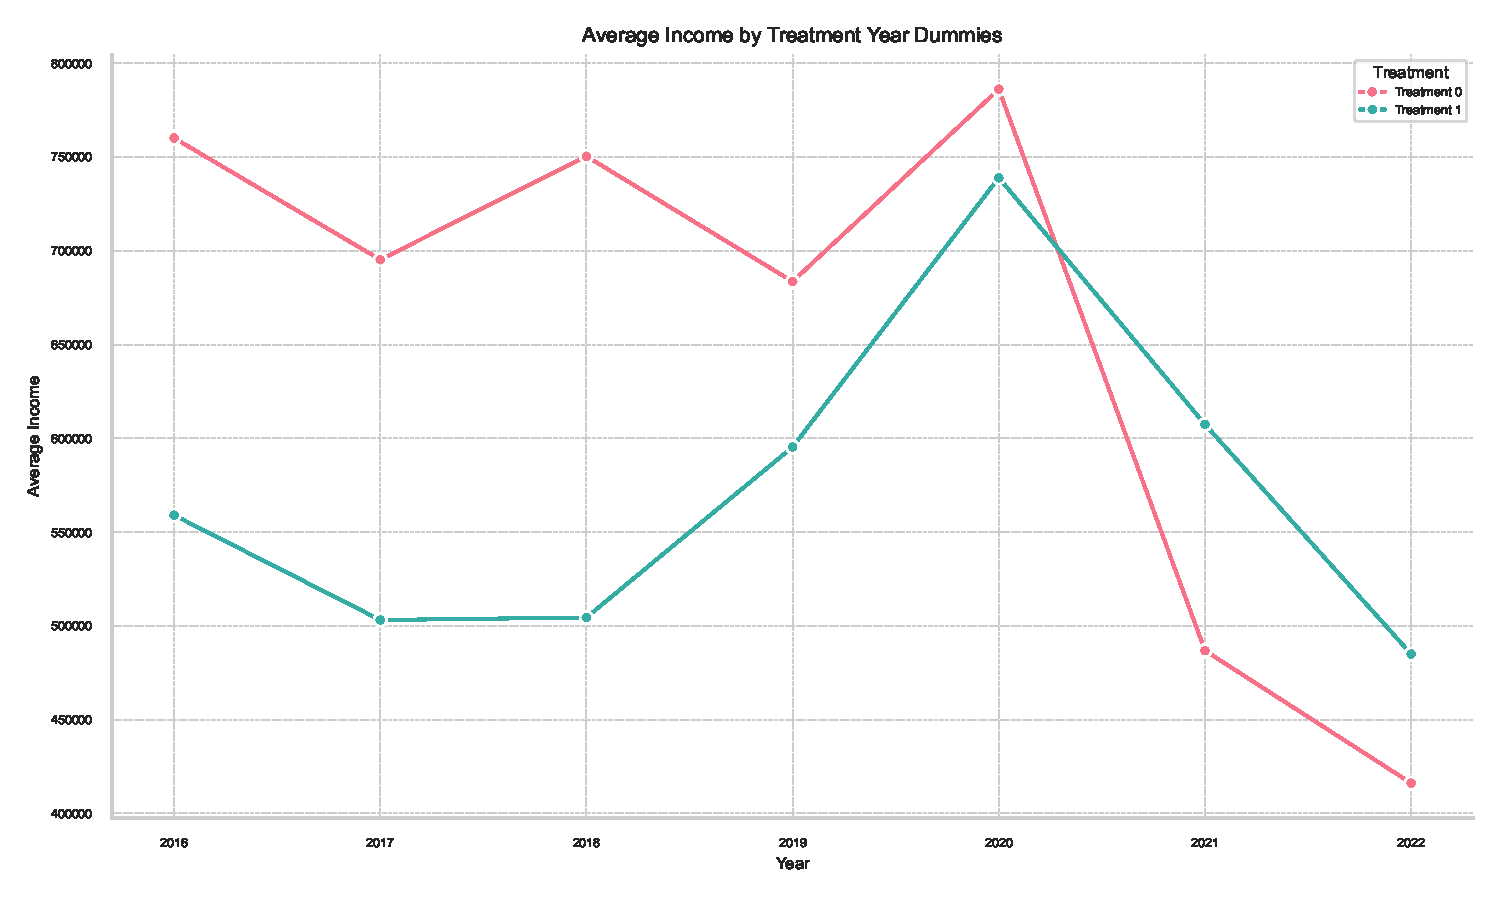
\includegraphics[width=0.7\textwidth]{../figures/average_income_by_treatment_platform.pdf}
    \caption{Treatment Effect of Platform Consolidation}
    \label{fig:treatment_consolidation}
    Note: the x-axis is year and the y-axis is the average income of Lianjia in each year. The graph uses the neighborhood-level data.
\end{figure}

\newpage


\subsection{Robustness Check by Dividing the Samples to Low and High Nighttime Lights} \label{subsec:nighttime_light_robustness_check}


Table \ref{tab:robustness_nighttime_light_entry} and Table \ref{tab:robustness_nighttime_light_consolidation} show the additional results of the DID model by classifying the samples to low and high nighttime light areas. The results show that there is heterogeneity effect across different areas, but the general estimation results are in line with our main model.

\begin{table}[H]
  \begin{center}
    \begin{scriptsize}
      \caption{Robustness Check for Offline Expansion Effect Using Nighttime Lights}
      \label{tab:robustness_nighttime_light_entry}
      {
\def\sym#1{\ifmmode^{#1}\else\(^{#1}\)\fi}
\begin{adjustbox}{max width=\textwidth}
\begin{tabular}{l*{8}{c}}
\toprule
            &\multicolumn{1}{c}{(1)}&\multicolumn{1}{c}{(2)}&\multicolumn{1}{c}{(3)}&\multicolumn{1}{c}{(4)}&\multicolumn{1}{c}{(5)}&\multicolumn{1}{c}{(6)}&\multicolumn{1}{c}{(7)}&\multicolumn{1}{c}{(8)}\\
            &\multicolumn{1}{c}{log(number)}&\multicolumn{1}{c}{log(number)}&\multicolumn{1}{c}{log(lead times)}&\multicolumn{1}{c}{log(lead times)}&\multicolumn{1}{c}{log(negotiation period)}&\multicolumn{1}{c}{log(negotiation period)}&\multicolumn{1}{c}{price concession}&\multicolumn{1}{c}{price concession}\\
&[lower]&[higher]&[lower]&[higher]&[lower]&[higher]&[lower]&[higher]\\
\midrule
pre2        &      -0.014         &       0.012         &      -0.010         &      -0.011         &      -0.042\sym{**} &      -0.010         &      -0.064\sym{*}  &       0.044         \\
            &     (0.020)         &     (0.023)         &     (0.016)         &     (0.017)         &     (0.017)         &     (0.026)         &     (0.033)         &     (0.047)         \\
\addlinespace
entry       &       0.109\sym{***}&       0.076\sym{***}&       0.027\sym{**} &       0.027\sym{**} &      -0.016         &      -0.020         &       0.078\sym{***}&       0.052         \\
            &     (0.018)         &     (0.017)         &     (0.013)         &     (0.013)         &     (0.014)         &     (0.016)         &     (0.026)         &     (0.036)         \\
\addlinespace
post1       &       0.055\sym{***}&       0.051\sym{***}&       0.052\sym{***}&       0.017         &      -0.023         &       0.001         &       0.048         &       0.028         \\
            &     (0.020)         &     (0.018)         &     (0.014)         &     (0.015)         &     (0.015)         &     (0.015)         &     (0.032)         &     (0.035)         \\
\addlinespace
post2       &       0.001         &       0.005         &      -0.006         &       0.032\sym{**} &      -0.006         &       0.013         &       0.025         &       0.000         \\
            &     (0.021)         &     (0.019)         &     (0.016)         &     (0.016)         &     (0.015)         &     (0.017)         &     (0.034)         &     (0.042)         \\
\addlinespace
post3       &      -0.030         &       0.042\sym{**} &       0.004         &       0.034\sym{**} &      -0.032         &       0.008         &       0.040         &       0.039         \\
            &     (0.023)         &     (0.020)         &     (0.017)         &     (0.015)         &     (0.020)         &     (0.019)         &     (0.036)         &     (0.048)         \\
\addlinespace
Brokerage Control &  \checkmark         &  \checkmark         &  \checkmark         &  \checkmark         &  \checkmark         &  \checkmark         &  \checkmark         &  \checkmark         \\
\addlinespace
Hedonic Control &  \checkmark         &  \checkmark         &  \checkmark         &  \checkmark         &  \checkmark         &  \checkmark         &  \checkmark         &  \checkmark         \\
\addlinespace
Transaction Control &  \checkmark         &  \checkmark         &  \checkmark         &  \checkmark         &  \checkmark         &  \checkmark         &  \checkmark         &  \checkmark         \\
\addlinespace
Regional Control &  \checkmark         &  \checkmark         &  \checkmark         &  \checkmark         &  \checkmark         &  \checkmark         &  \checkmark         &  \checkmark         \\
\midrule
\(N\)       &       51617         &       46404         &       51617         &       46404         &      492451         &      373389         &      479061         &      364862         \\
R-squared   &       0.837         &       0.823         &       0.917         &       0.919         &       0.515         &       0.525         &       0.231         &       0.259         \\
\bottomrule
\multicolumn{9}{l}{\footnotesize Standard errors in parentheses}\\
\multicolumn{9}{l}{\footnotesize \sym{*} \(p<0.1\), \sym{**} \(p<0.05\), \sym{***} \(p<0.01\)}\\
\end{tabular}
\end{adjustbox}
}

    
    Note: we omit all the control variables in the regression model, and detailed descriptions can be seen from Table \ref{tab:statistical_district} and Table \ref{tab:statistical_individual}.
    \end{scriptsize}
  \end{center}
\end{table}

\begin{table}[H]
  \begin{center}
    \begin{scriptsize}
      \caption{Robustness Check for Platform Consolidation Effect using Nighttime Lights}
      \label{tab:robustness_nighttime_light_consolidation}
      {
\def\sym#1{\ifmmode^{#1}\else\(^{#1}\)\fi}
\begin{adjustbox}{max width=\textwidth}
\begin{tabular}{l*{8}{c}}
\toprule
            &\multicolumn{1}{c}{(1)}&\multicolumn{1}{c}{(2)}&\multicolumn{1}{c}{(3)}&\multicolumn{1}{c}{(4)}&\multicolumn{1}{c}{(5)}&\multicolumn{1}{c}{(6)}&\multicolumn{1}{c}{(7)}&\multicolumn{1}{c}{(8)}\\
            &\multicolumn{1}{c}{log(number)}&\multicolumn{1}{c}{log(number)}&\multicolumn{1}{c}{log(lead times)}&\multicolumn{1}{c}{log(lead times)}&\multicolumn{1}{c}{log(negotiation period)}&\multicolumn{1}{c}{log(negotiation period)}&\multicolumn{1}{c}{price concession}&\multicolumn{1}{c}{price concession}\\
&[lower]&[higher]&[lower]&[higher]&[lower]&[higher]&[lower]&[higher]\\
\midrule
pre1\_treatment&       0.002         &       0.000         &       0.006         &       0.013         &      -0.010         &      -0.024\sym{*}  &       0.012         &       0.007         \\
            &     (0.015)         &     (0.014)         &     (0.012)         &     (0.012)         &     (0.012)         &     (0.014)         &     (0.029)         &     (0.033)         \\
\addlinespace
treatment   &       0.016         &      -0.013         &      -0.015         &       0.010         &      -0.020         &       0.003         &       0.016         &       0.009         \\
            &     (0.015)         &     (0.015)         &     (0.012)         &     (0.012)         &     (0.015)         &     (0.015)         &     (0.028)         &     (0.036)         \\
\addlinespace
post1\_treatment&       0.073\sym{***}&       0.044\sym{**} &       0.020         &       0.055\sym{***}&      -0.007         &      -0.016         &       0.068\sym{**} &       0.058         \\
            &     (0.018)         &     (0.018)         &     (0.014)         &     (0.013)         &     (0.018)         &     (0.017)         &     (0.033)         &     (0.043)         \\
\addlinespace
post2\_treatment&       0.057\sym{***}&       0.059\sym{***}&       0.015         &       0.057\sym{***}&      -0.011         &      -0.002         &       0.100\sym{**} &       0.051         \\
            &     (0.020)         &     (0.020)         &     (0.015)         &     (0.016)         &     (0.020)         &     (0.018)         &     (0.041)         &     (0.053)         \\
\addlinespace
post3\_treatment&       0.021         &       0.016         &       0.017         &       0.009         &      -0.000         &      -0.016         &       0.044         &       0.059         \\
            &     (0.024)         &     (0.026)         &     (0.018)         &     (0.022)         &     (0.024)         &     (0.022)         &     (0.052)         &     (0.070)         \\
\addlinespace
Brokerage Control &  \checkmark         &  \checkmark         &  \checkmark         &  \checkmark         &  \checkmark         &  \checkmark         &  \checkmark         &  \checkmark         \\
\addlinespace
Hedonic Control &  \checkmark         &  \checkmark         &  \checkmark         &  \checkmark         &  \checkmark         &  \checkmark         &  \checkmark         &  \checkmark         \\
\addlinespace
Transaction Control &  \checkmark         &  \checkmark         &  \checkmark         &  \checkmark         &  \checkmark         &  \checkmark         &  \checkmark         &  \checkmark         \\
\addlinespace
Regional Control &  \checkmark         &  \checkmark         &  \checkmark         &  \checkmark         &  \checkmark         &  \checkmark         &  \checkmark         &  \checkmark         \\
\midrule
\(N\)       &       69000         &       56419         &       69000         &       56419         &      770057         &      496170         &      756841         &      487490         \\
R-squared   &       0.870         &       0.849         &       0.927         &       0.931         &       0.541         &       0.539         &       0.238         &       0.274         \\
\bottomrule
\multicolumn{9}{l}{\footnotesize Standard errors in parentheses}\\
\multicolumn{9}{l}{\footnotesize \sym{*} \(p<0.1\), \sym{**} \(p<0.05\), \sym{***} \(p<0.01\)}\\
\end{tabular}
\end{adjustbox}
}

    
    Note: we omit all the control variables in the regression model, and detailed descriptions can be seen from Table \ref{tab:statistical_district} and Table \ref{tab:statistical_individual}.
    \end{scriptsize}
  \end{center}
\end{table}

\subsection{Placebo Test} \label{subsec:placebo_test}

Figure \ref{fig:placebo_test_entry} and Figure \ref{fig:placebo_test_plat} show the results of the placebo test for the entry effect and the platform consolidation effect. The results show that the random treatment effect is non-significant at the 10\% level, indicating that the treatment effect is not due to other factors.

\begin{figure}[H]
  \centering
  \subfloat[Placebo Test to transaction number]{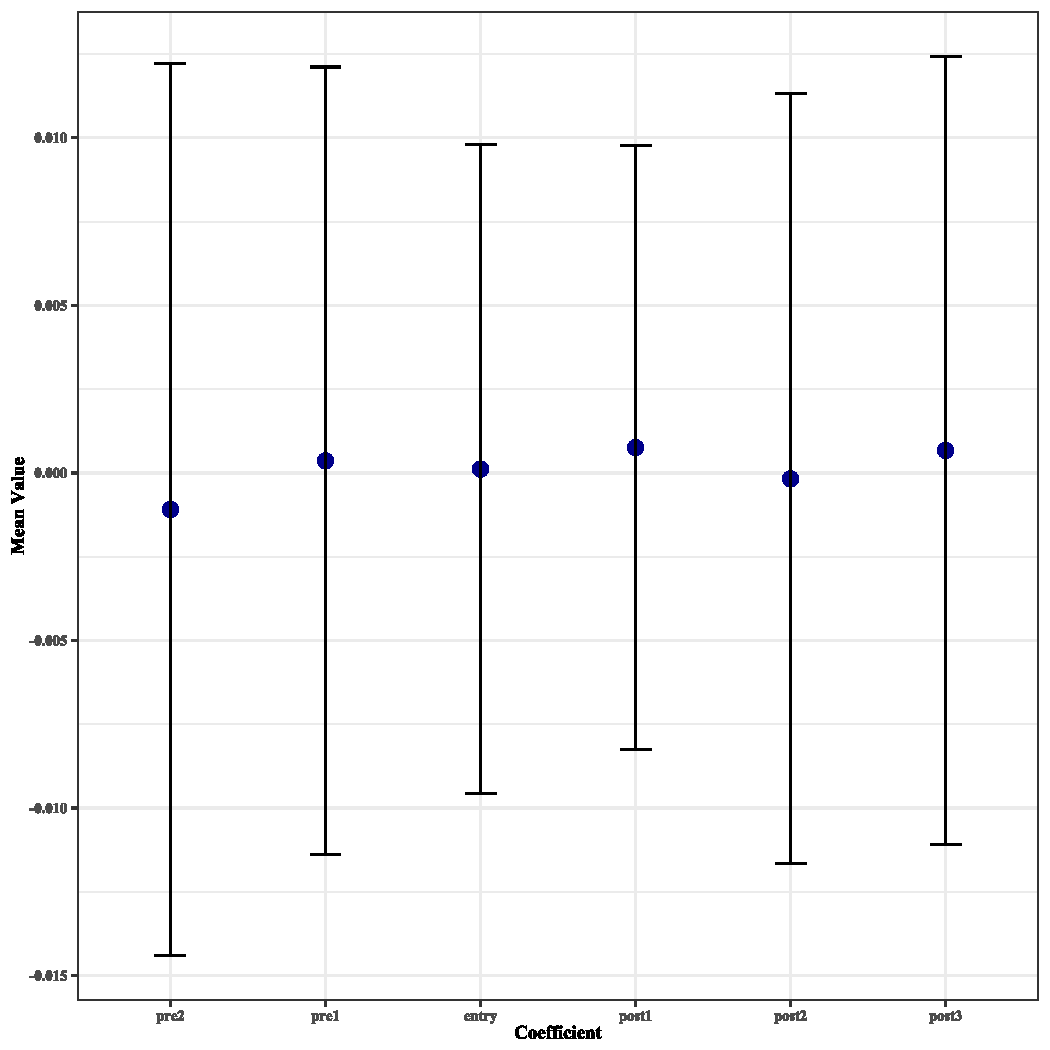
\includegraphics[width=0.45\textwidth]{../figures/placebo_results/placebo_entry_num.pdf}\label{fig:placebo_num_entry}}
  \subfloat[Placebo Test to number of house tours]{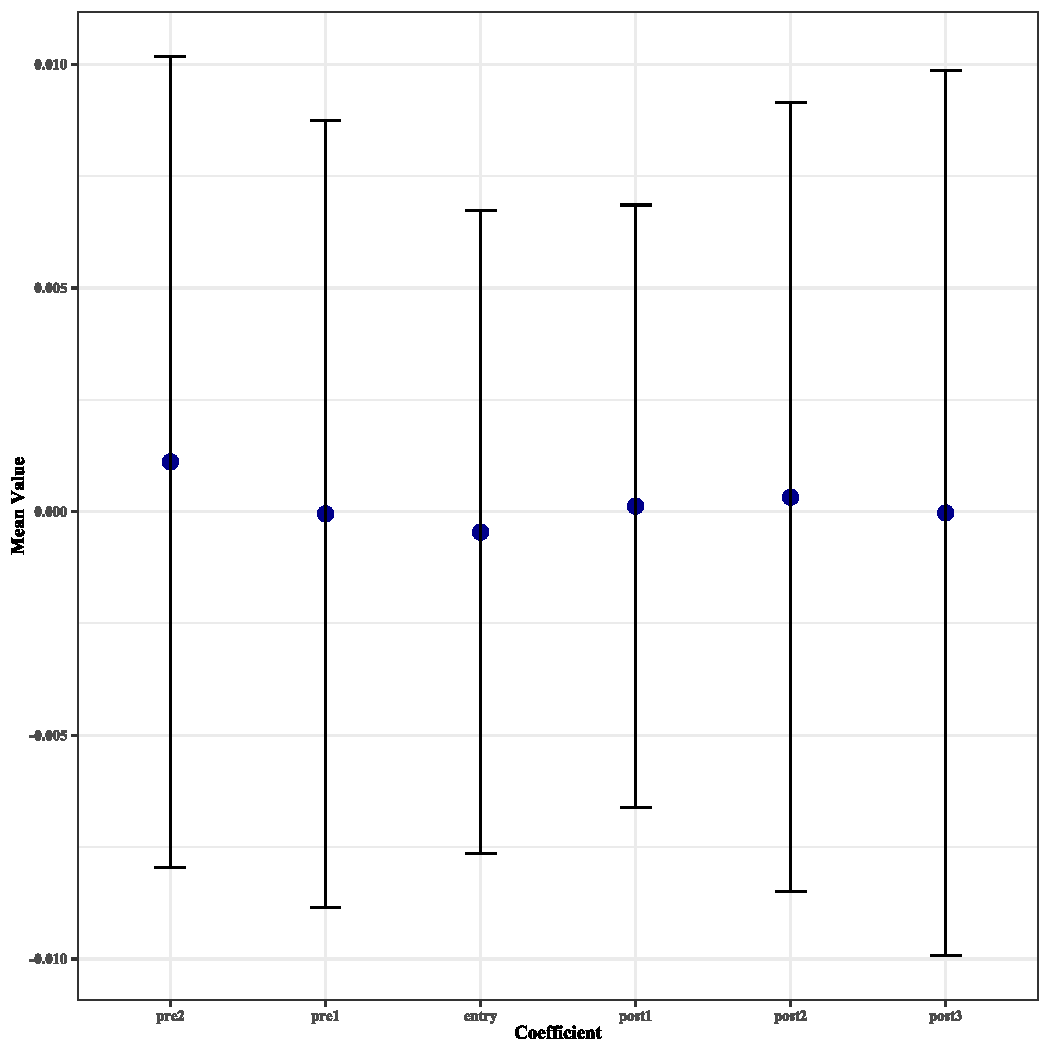
\includegraphics[width=0.45\textwidth]{../figures/placebo_results/placebo_entry_lead.pdf}\label{fig:placebo_lead_entry}}
  \hfill % Adds horizontal space between figures
  \subfloat[Placebo Test to transaction period]{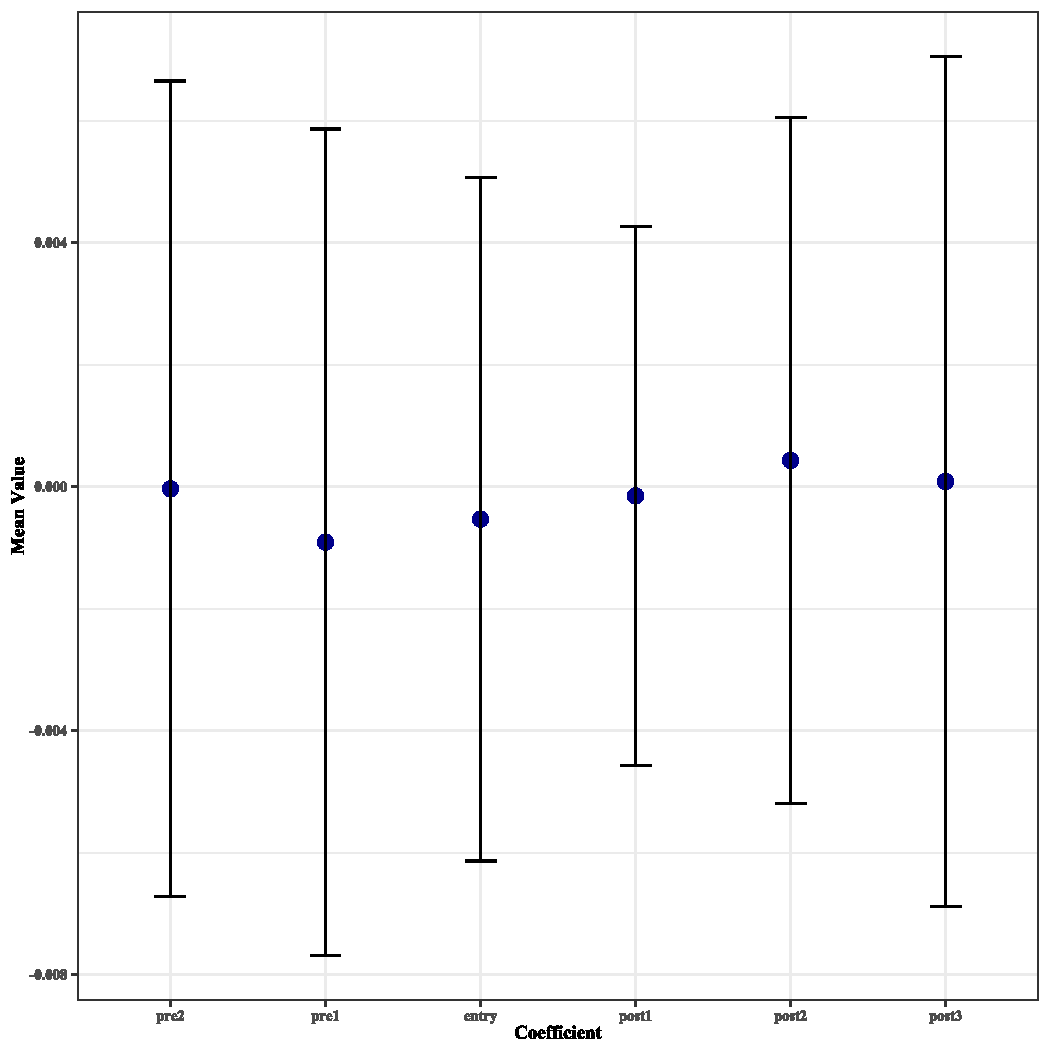
\includegraphics[width=0.45\textwidth]{../figures/placebo_results/placebo_entry_period.pdf}\label{fig:placebo_period_entry}}
  \subfloat[Placebo Test to price concession]{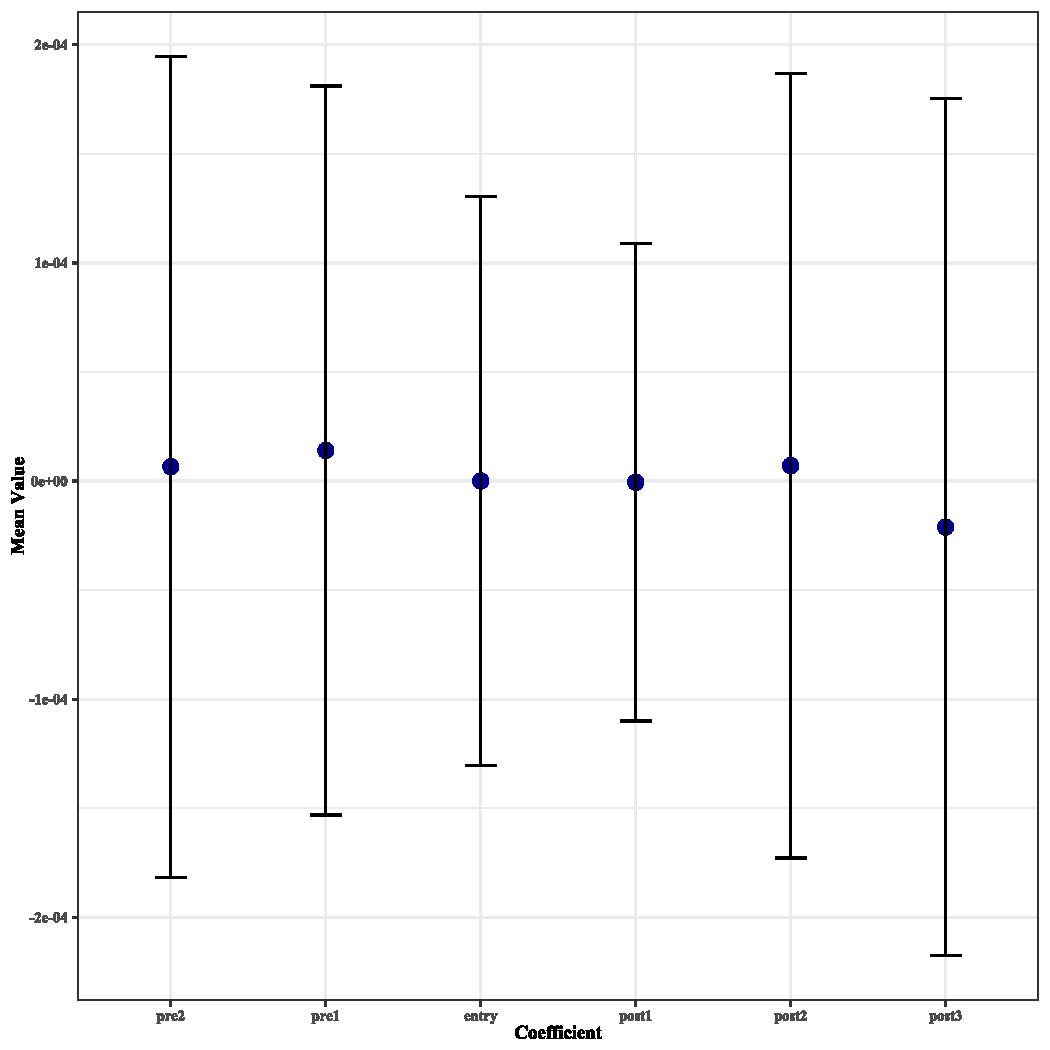
\includegraphics[width=0.45\textwidth]{../figures/placebo_results/placebo_entry_concession.pdf}\label{fig:placebo_concession_entry}}
  \caption{Placebo Test to Entry Effect}
  \label{fig:placebo_test_entry}

  Note: The x-axis is the coefficient of the 

  the model is described in Equation \eqref{eq:entry_effect}
  \end{figure}

\begin{figure}[H]
  \centering
  \subfloat[Placebo Test to transaction number]{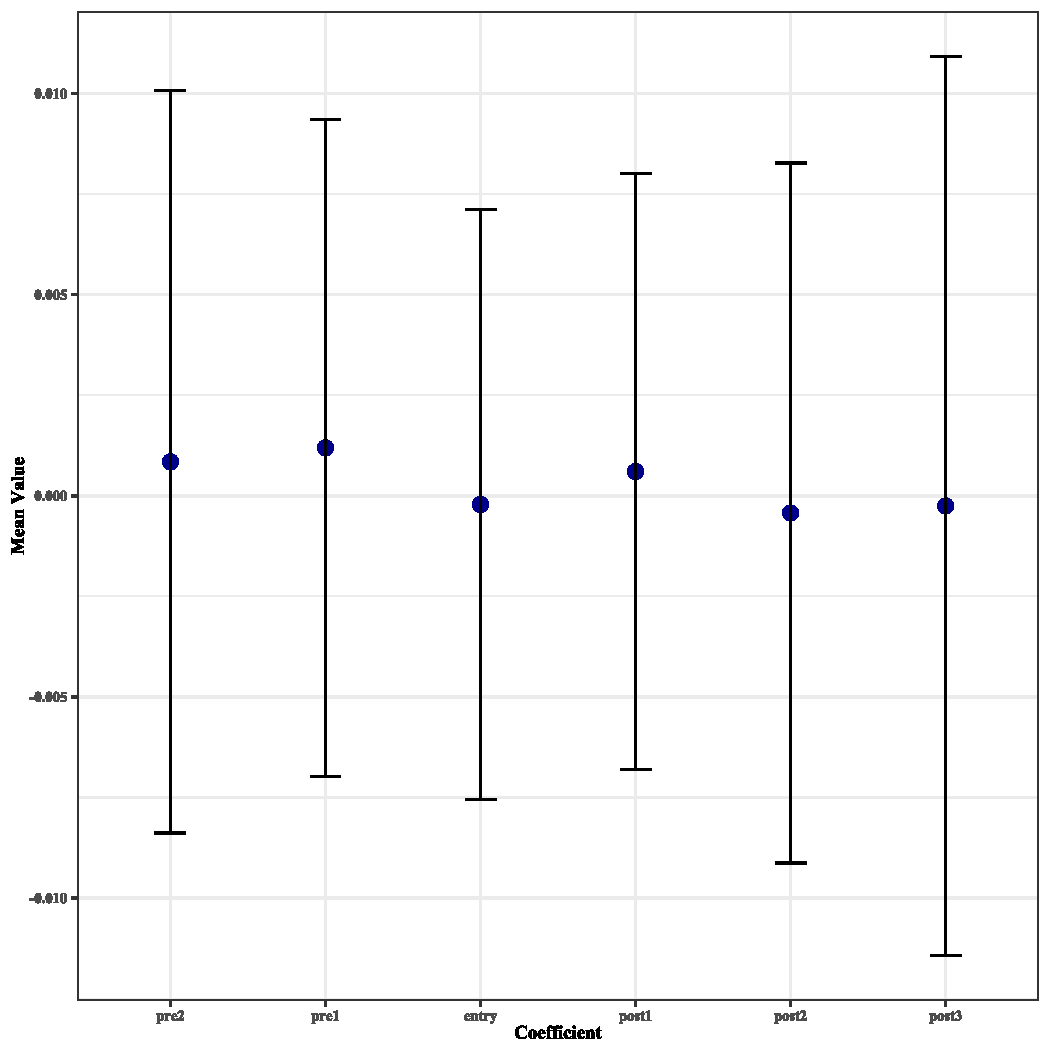
\includegraphics[width=0.45\textwidth]{../figures/placebo_results/placebo_plat_num.pdf}\label{fig:placebo_num_plat}}
  \subfloat[Placebo Test to number of house tours]{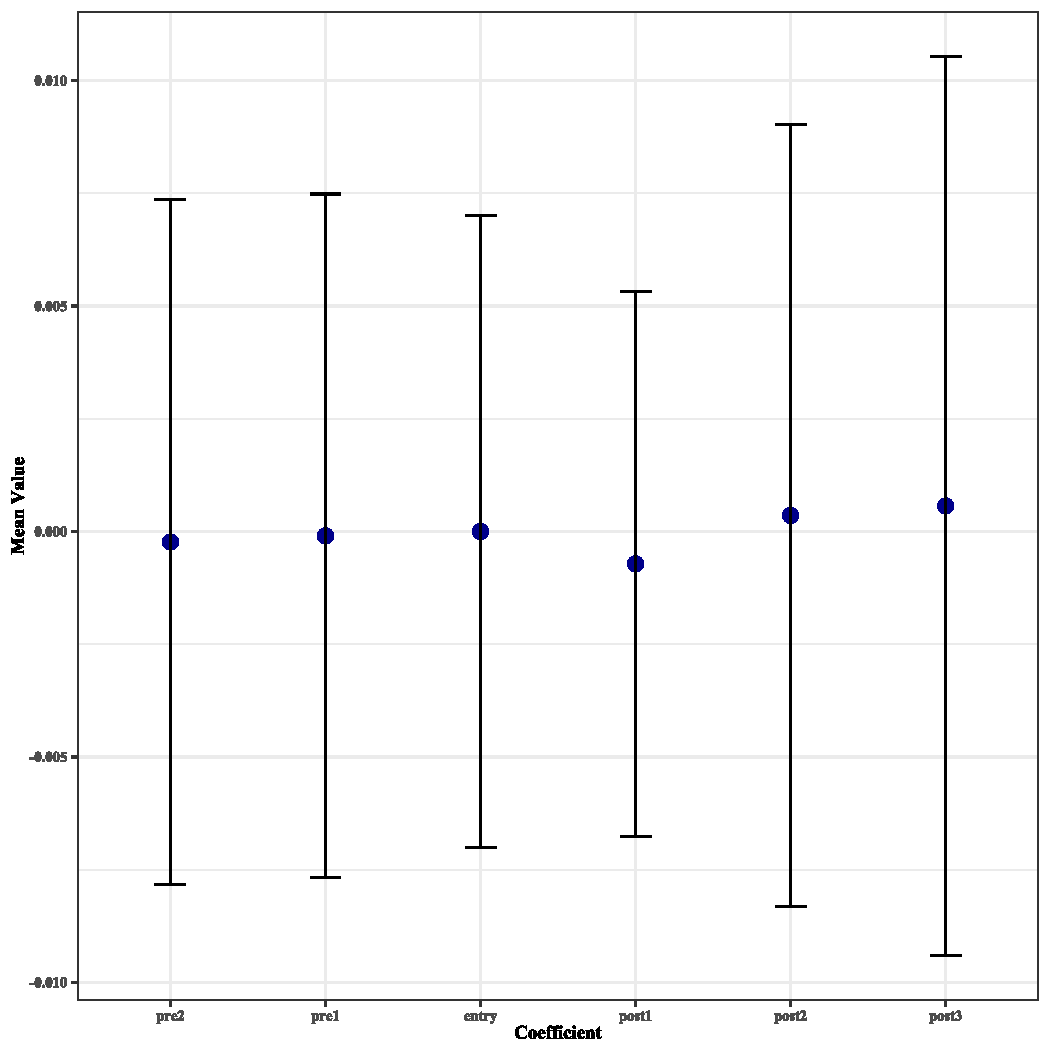
\includegraphics[width=0.45\textwidth]{../figures/placebo_results/placebo_plat_lead.pdf}\label{fig:placebo_lead_plat}}
  \hfill % Adds horizontal space between figures
  \subfloat[Placebo Test to transaction period]{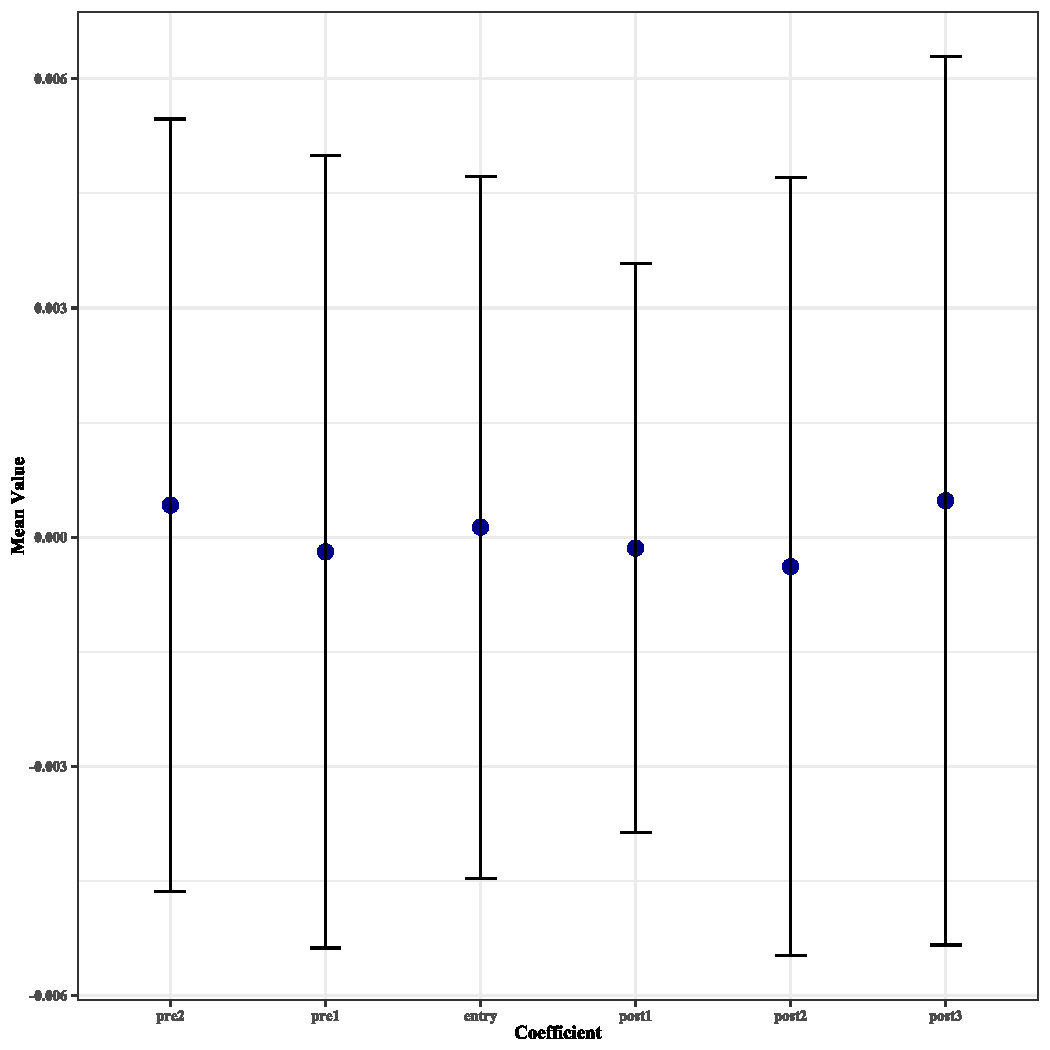
\includegraphics[width=0.45\textwidth]{../figures/placebo_results/placebo_plat_period.pdf}\label{fig:placebo_period_plat}}
  \subfloat[Placebo Test to price concession]{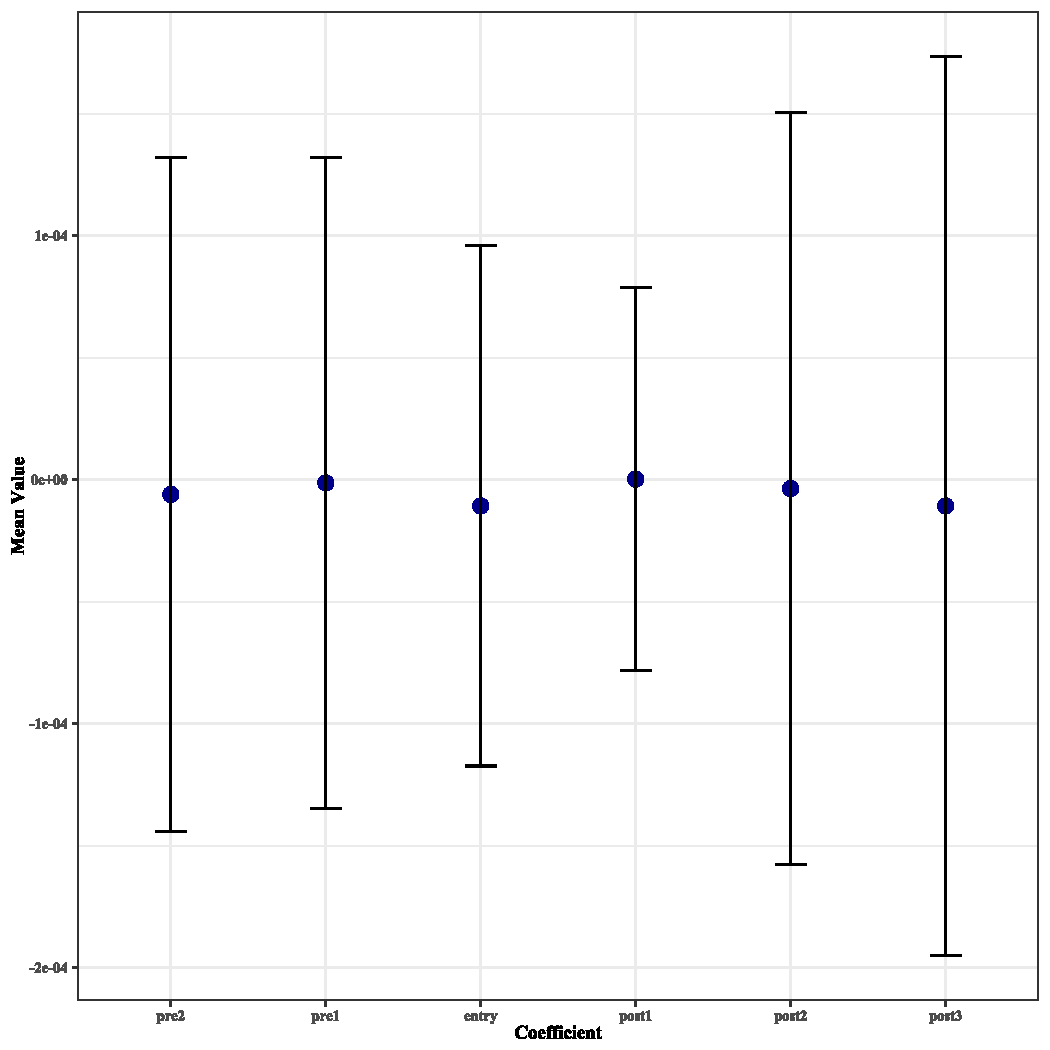
\includegraphics[width=0.45\textwidth]{../figures/placebo_results/placebo_plat_concession.pdf}\label{fig:placebo_concession_plat}}
  \caption{Placebo Test to Platform-Mediated Consolidation Effect}
  \label{fig:placebo_test_plat}

  Note: The x-axis is the coefficient of the 

  the model is described in Equation \eqref{eq:acn_assessment}

\end{figure}

\newpage

\section{Description of the network effect indices} \label{sec:network_effect_indices}

\subsection{Descriptions of the clustering indices} \label{subsec:descriptions_clustering_indices}

We also provide a descriptions of the measures of the clustering coefficient effects:

We also calcualted the the local clustering coefficient for a node $i$, which is a measure of the likelihood that the neighbors of $i$ are also neighbors of each other, and it is calcualted as:

\begin{equation*}
  C_i = \frac{2e_i}{k_i(k_i - 1)}  
\end{equation*}

where $e_i$ is the number of edges between the neighbors of node $i$ and $k_i$ is the degree of node $i$. The average clustering coefficient is the mean of the local clustering coefficients for all nodes in the network, defined as: $C = \frac{1}{n} \sum_{i=1}^n C_i$ where $n$ is the total number of nodes. This index indicates how close the neighbors of a node are to forming a complete graph (clique).

The global clustering coefficient, also known as transitivity, is a measure of the overall tendency of the network to form triangles. It is defined as the ratio of the number of closed triplets (triangles) to the number of all triplets (both open and closed) in the network.

\begin{equation*}
  C_g = \frac{3 \times \text{number of closed triplets}}{\text{number of all triplets}}  
\end{equation*}

A triplet consists of three nodes connected by either two (open triplet) or three (closed triplet) edges. This index indicates the global interconnectedness and the presence of tightly knit groups within the entire network. For both indices, higher values indicate a denser network. Typically, values between 0.75 and 1 signify a dense network, values between 0.4 and 0.7 indicate a moderately dense network, and values between 0 and 0.3 represent a sparse network.

\subsection{Other Indices Measures} \label{subsec:other_indices_measures}

We also consider other indices that describes the network formation using degree centrality, betweenness centrality, closeness centrality and page rank:

Degree centrality measures the number of direct connections a node has to other nodes in the network. It is defined as:

\begin{equation*}
  C_D(v) = \frac{d(v)}{n - 1}
\end{equation*}

where $d(v)$ is the degree of node $v$, and $n$ is the total number of nodes in the network. A higher degree centrality indicates that a node has more direct connections and may be considered more influential or important within the network.

Closeness centrality measures how close a node is to all other nodes in the network, based on the shortest paths. It is given by:

\begin{equation*}
  C_C(v) = \frac{n - 1}{\sum_{u \neq v} d(u, v)}
\end{equation*}

where $d(u, v)$ is the shortest path distance between nodes $u$ and $v$. A higher closeness centrality indicates that a node can reach other nodes more quickly, signifying a more central position within the network.

PageRank is a measure of the importance of nodes in a network, originally developed for ranking web pages. It is calculated using the following iterative formula:

\begin{equation*}
  PR(v) = \frac{1 - d}{n} + d\sum_{u \in M(v)} \frac{PR(u)}{L(u)}
\end{equation*}

where $d$ is a damping factor (typically set to $0.85$), $M(v)$ is the set of nodes that link to $v$, $L(u)$ is the number of outbound links from node $u$. Nodes with high PageRank scores are considered to have high influence and are often central to the network's structure.

The results also indicate that the local network effect of Lianjia tends to be sparse and the network is not well-connected. The network effect is primarily characterized by local clustering, with moderate network strength.

\begin{table}[H]
  \begin{center}
  \caption{Closeness Centrality}
  \label{other:closeness_centrality}
  \caption{Panel A: max(closeness centrality)}
\begin{tabular}{lrrrrrll}
\hline
 city      &   2016 &   2017 &   2018 &   2019 &   2020 & 2021   & 2022   \\
\hline
 Beijing   & 0.0174 & 0.0259 & 0.0315 & 0.0338 & 0.035  &        &        \\
 Chengdu   & 0.1365 & 0.2231 & 0.2291 & 0.2675 & 0.282  &        &        \\
 Chongqing & 0.029  & 0.0469 & 0.0483 & 0.0543 & 0.0986 & 0.1006 & 0.0986 \\
 Guangzhou & 0.0317 & 0.0289 & 0.0359 & 0.0357 & 0.0308 & 0.1021 & 0.0932 \\
 Hangzhou  & 0.0556 & 0.0791 & 0.0652 & 0.0584 & 0.085  & 0.0527 & 0.0650 \\
 Nanjing   & 0.0493 & 0.1133 & 0.0868 & 0.1626 & 0.2083 & 0.2073 & 0.1841 \\
 Shanghai  & 0.1132 & 0.0682 & 0.0835 & 0.1024 & 0.0449 & 0.0944 & 0.0376 \\
 Shenzhen  & 0.0362 & 0.0453 & 0.0485 & 0.0379 & 0.0863 &        &        \\
 Tianjin   & 0.0481 & 0.0407 & 0.0371 & 0.0961 & 0.1688 & 0.1837 & 0.1838 \\
 Wuhan     & 0.0259 & 0.0509 & 0.0491 & 0.0357 & 0.0642 &        &        \\
\hline
\end{tabular}

\caption{Panel B: mean(closeness centrality)}
\begin{tabular}{lrrrrrll}
\hline
 city      &   2016 &   2017 &   2018 &   2019 &   2020 & 2021   & 2022   \\
\hline
 Beijing   & 0.0015 & 0.0024 & 0.0025 & 0.0023 & 0.0031 &        &        \\
 Chengdu   & 0.015  & 0.032  & 0.0336 & 0.042  & 0.0415 &        &        \\
 Chongqing & 0.0031 & 0.0036 & 0.0039 & 0.0036 & 0.0073 & 0.0071 & 0.0070 \\
 Guangzhou & 0.0031 & 0.0034 & 0.0029 & 0.0038 & 0.0026 & 0.0079 & 0.0071 \\
 Hangzhou  & 0.0056 & 0.0076 & 0.0055 & 0.0047 & 0.0068 & 0.0039 & 0.0042 \\
 Shenzhen  & 0.003  & 0.0042 & 0.0042 & 0.0039 & 0.0079 &        &        \\
 Shanghai  & 0.0089 & 0.0045 & 0.0064 & 0.0071 & 0.0032 & 0.0060 & 0.0028 \\
 Tianjin   & 0.0053 & 0.0045 & 0.0041 & 0.0071 & 0.0146 & 0.0165 & 0.0164 \\
 Wuhan     & 0.0028 & 0.0039 & 0.003  & 0.0027 & 0.0058 &        &        \\
 Nanjing   & 0.0045 & 0.0113 & 0.008  & 0.0158 & 0.0229 & 0.0202 & 0.0166 \\
\hline
\end{tabular}

\caption{Panel C: median(closeness centrality)}
\begin{tabular}{lrrrrrll}
\hline
 city      &   2016 &   2017 &   2018 &   2019 &   2020 & 2021   & 2022   \\
\hline
 Guangzhou & 0.0003 & 0.0002 & 0.0002 & 0.0002 & 0.0001 & 0.0001 & 0.0001 \\
 Beijing   & 0.0001 & 0      & 0      & 0      & 0      &        &        \\
 Chengdu   & 0.0001 & 0.0001 & 0.0001 & 0      & 0      &        &        \\
 Chongqing & 0.0003 & 0.0002 & 0.0002 & 0.0001 & 0.0001 & 0.0001 & 0.0001 \\
 Hangzhou  & 0.0003 & 0.0002 & 0.0002 & 0.0001 & 0.0001 & 0.0001 & 0.0001 \\
 Shenzhen  & 0.0002 & 0.0001 & 0.0001 & 0.0001 & 0.0001 &        &        \\
 Shanghai  & 0      & 0      & 0      & 0      & 0      & 0.0000 & 0.0000 \\
 Tianjin   & 0.0001 & 0.0001 & 0.0001 & 0.0001 & 0.0001 & 0.0001 & 0.0001 \\
 Wuhan     & 0.0004 & 0.0002 & 0.0002 & 0.0001 & 0.0001 &        &        \\
 Nanjing   & 0.0002 & 0.0001 & 0.0001 & 0.0001 & 0.0001 & 0.0001 & 0.0001 \\
\hline
\end{tabular}
\end{center}
\end{table}

\begin{table}[H]
  \begin{center}
  \caption{Degree Centrality}
  \label{other:degree_centrality}
  \caption{Panel D: max(degree centrality)}
\begin{tabular}{lrrrrrll}
\hline
 city      &   2016 &   2017 &   2018 &   2019 &   2020 & 2021   & 2022   \\
\hline
 Beijing   & 0.0029 & 0.0026 & 0.0027 & 0.0026 & 0.0025 &        &        \\
 Chengdu   & 0.0075 & 0.0064 & 0.0063 & 0.0055 & 0.0061 &        &        \\
 Chongqing & 0.0118 & 0.0121 & 0.0098 & 0.0067 & 0.0052 & 0.0052 & 0.0051 \\
 Guangzhou & 0.0207 & 0.0096 & 0.0121 & 0.0101 & 0.006  & 0.0060 & 0.0061 \\
 Hangzhou  & 0.0126 & 0.0096 & 0.0095 & 0.0079 & 0.0076 & 0.0060 & 0.0065 \\
 Shanghai  & 0.0045 & 0.0034 & 0.0033 & 0.0038 & 0.0038 & 0.0034 & 0.0036 \\
 Shenzhen  & 0.0084 & 0.0076 & 0.0078 & 0.0081 & 0.0075 &        &        \\
 Tianjin   & 0.0092 & 0.0081 & 0.0074 & 0.007  & 0.0079 & 0.0092 & 0.0093 \\
 Wuhan     & 0.0141 & 0.0119 & 0.0105 & 0.0082 & 0.0064 &        &        \\
 Nanjing   & 0.0078 & 0.0071 & 0.0077 & 0.0074 & 0.0069 & 0.0069 & 0.0073 \\
\hline
\end{tabular}

\caption{Panel E: mean(degree centrality)}
\begin{tabular}{lrrrrrll}
\hline
 city      &   2016 &   2017 &   2018 &   2019 &   2020 & 2021   & 2022   \\
\hline
 Shanghai  & 0.0002 & 0.0002 & 0.0002 & 0.0002 & 0.0002 & 0.0002 & 0.0002 \\
 Wuhan     & 0.0009 & 0.0007 & 0.0007 & 0.0005 & 0.0005 &        &        \\
 Tianjin   & 0.0004 & 0.0005 & 0.0004 & 0.0004 & 0.0004 & 0.0005 & 0.0005 \\
 Shenzhen  & 0.0005 & 0.0006 & 0.0005 & 0.0005 & 0.0005 &        &        \\
 Nanjing   & 0.0005 & 0.0006 & 0.0006 & 0.0005 & 0.0005 & 0.0005 & 0.0005 \\
 Hangzhou  & 0.0008 & 0.0006 & 0.0006 & 0.0005 & 0.0005 & 0.0005 & 0.0005 \\
 Guangzhou & 0.0007 & 0.0006 & 0.0007 & 0.0007 & 0.0004 & 0.0005 & 0.0005 \\
 Chongqing & 0.0007 & 0.0007 & 0.0006 & 0.0004 & 0.0004 & 0.0004 & 0.0004 \\
 Chengdu   & 0.0003 & 0.0003 & 0.0003 & 0.0003 & 0.0002 &        &        \\
 Beijing   & 0.0002 & 0.0002 & 0.0002 & 0.0002 & 0.0002 &        &        \\
\hline
\end{tabular}

\caption{Panel F: median(degree centrality)}
\begin{tabular}{lrrrrrll}
\hline
 city      &   2016 &   2017 &   2018 &   2019 &   2020 & 2021   & 2022   \\
\hline
 Beijing   & 0.0001 & 0      & 0      & 0      & 0      &        &        \\
 Chengdu   & 0.0001 & 0.0001 & 0.0001 & 0      & 0      &        &        \\
 Chongqing & 0.0003 & 0.0002 & 0.0002 & 0.0001 & 0.0001 & 0.0001 & 0.0001 \\
 Guangzhou & 0.0003 & 0.0002 & 0.0002 & 0.0002 & 0.0001 & 0.0001 & 0.0001 \\
 Hangzhou  & 0.0003 & 0.0002 & 0.0002 & 0.0001 & 0.0001 & 0.0001 & 0.0001 \\
 Nanjing   & 0.0002 & 0.0001 & 0.0001 & 0.0001 & 0.0001 & 0.0001 & 0.0001 \\
 Shanghai  & 0      & 0      & 0      & 0      & 0      & 0.0000 & 0.0000 \\
 Shenzhen  & 0.0002 & 0.0001 & 0.0001 & 0.0001 & 0.0001 &        &        \\
 Tianjin   & 0.0001 & 0.0001 & 0.0001 & 0.0001 & 0.0001 & 0.0001 & 0.0001 \\
 Wuhan     & 0.0004 & 0.0002 & 0.0002 & 0.0001 & 0.0001 &        &        \\
\hline
\end{tabular}
\end{center}
\end{table}

\begin{table}[H]
  \begin{center}
  \caption{Page Rank}
  \label{other:page_rank}
  \caption{Panel G: max(page rank)}
\begin{tabular}{lrrrrrll}
\hline
 city      &   2016 &   2017 &   2018 &   2019 &   2020 & 2021   & 2022   \\
\hline
 Beijing   & 0.0014 & 0.0011 & 0.0011 & 0.001  & 0.0007 &        &        \\
 Chengdu   & 0.0036 & 0.0025 & 0.0021 & 0.0018 & 0.0011 &        &        \\
 Guangzhou & 0.0102 & 0.0041 & 0.0042 & 0.0059 & 0.0024 & 0.0012 & 0.0011 \\
 Hangzhou  & 0.0067 & 0.0042 & 0.0034 & 0.0042 & 0.0016 & 0.0015 & 0.0016 \\
 Chongqing & 0.0085 & 0.0069 & 0.0045 & 0.0034 & 0.0019 & 0.0014 & 0.0011 \\
 Shanghai  & 0.0011 & 0.0013 & 0.001  & 0.0008 & 0.001  & 0.0018 & 0.0013 \\
 Shenzhen  & 0.0046 & 0.0023 & 0.0024 & 0.0037 & 0.0012 &        &        \\
 Tianjin   & 0.0048 & 0.0038 & 0.0052 & 0.0043 & 0.0021 & 0.0017 & 0.0016 \\
 Wuhan     & 0.0085 & 0.0044 & 0.0032 & 0.0031 & 0.0011 &        &        \\
 Nanjing   & 0.005  & 0.0022 & 0.0024 & 0.0023 & 0.0016 & 0.0014 & 0.0011 \\
\hline
\end{tabular}

\caption{Panel H: mean(page rank)}
\begin{tabular}{lrrrrrll}
\hline
 city      &   2016 &   2017 &   2018 &   2019 &   2020 & 2021   & 2022   \\
\hline
 Beijing   & 0.0001 & 0.0001 & 0.0001 & 0.0001 & 0.0001 &        &        \\
 Chengdu   & 0.0001 & 0.0001 & 0.0001 & 0.0001 & 0.0001 &        &        \\
 Guangzhou & 0.0007 & 0.0003 & 0.0004 & 0.0004 & 0.0002 & 0.0001 & 0.0001 \\
 Hangzhou  & 0.0005 & 0.0004 & 0.0004 & 0.0003 & 0.0002 & 0.0002 & 0.0002 \\
 Chongqing & 0.0006 & 0.0005 & 0.0004 & 0.0003 & 0.0002 & 0.0001 & 0.0001 \\
 Shanghai  & 0.0001 & 0.0001 & 0.0001 & 0.0001 & 0.0001 & 0.0001 & 0.0001 \\
 Shenzhen  & 0.0003 & 0.0003 & 0.0003 & 0.0003 & 0.0002 &        &        \\
 Tianjin   & 0.0003 & 0.0003 & 0.0003 & 0.0002 & 0.0001 & 0.0001 & 0.0001 \\
 Wuhan     & 0.0007 & 0.0004 & 0.0003 & 0.0002 & 0.0001 &        &        \\
 Nanjing   & 0.0003 & 0.0003 & 0.0003 & 0.0002 & 0.0002 & 0.0001 & 0.0001 \\
\hline
\end{tabular}

\caption{Panel I: median(page rank)}
\begin{tabular}{lrrrrrll}
\hline
 city      &   2016 &   2017 &   2018 &   2019 &   2020 & 2021   & 2022   \\
\hline
 Tianjin   & 0.0001 & 0.0001 & 0.0001 & 0.0001 & 0      & 0.0000 & 0.0000 \\
 Beijing   & 0      & 0      & 0      & 0      & 0      &        &        \\
 Chengdu   & 0.0001 & 0      & 0      & 0      & 0      &        &        \\
 Chongqing & 0.0003 & 0.0002 & 0.0001 & 0.0001 & 0.0001 & 0.0000 & 0.0000 \\
 Guangzhou & 0.0003 & 0.0001 & 0.0001 & 0.0002 & 0.0001 & 0.0000 & 0.0000 \\
 Hangzhou  & 0.0002 & 0.0001 & 0.0001 & 0.0001 & 0.0001 & 0.0001 & 0.0001 \\
 Nanjing   & 0.0001 & 0.0001 & 0.0001 & 0.0001 & 0.0001 & 0.0000 & 0.0000 \\
 Shanghai  & 0      & 0      & 0      & 0      & 0      & 0.0000 & 0.0000 \\
 Shenzhen  & 0.0001 & 0.0001 & 0.0001 & 0.0001 & 0.0001 &        &        \\
 Wuhan     & 0.0003 & 0.0001 & 0.0001 & 0.0001 & 0      &        &        \\
\hline
\end{tabular}
\end{center}
\end{table}

\end{document}

% Freeman, L. C. (1977). A set of measures of centrality based on betweenness. Sociometry, 40(1), 35-41.
% Newman, M. E. J. (2010). Networks: An Introduction. Oxford University Press.
% Page, L., Brin, S., Motwani, R., & Winograd, T. (1999). The PageRank citation ranking: Bringing order to the web. Stanford InfoLab.
